\chapter{APPENDIX A.1}
\label{A1}
\vglue6pt

\begin{landscape}
\begin{table}[h!]
    \centering
    \caption{Cut-flow report showing number of events, before selections, in the semi-leptonic channel and in its categories. Percentages in brackets show the total selection efficiency that is number of events of the final state divided by the total number of events in the samples $\times 100$.}
\begin{tabular}{ |l|c|c|c|c|c|c| }
    \hline
    Samples                                & No sel.                   & Semi-leptonic F.S.               & DNN Cat. 1           & DNN Cat. 2          & DNN Cat. 3            & DNN Cat. 4            \\
    \hline
           $HH \rightarrow WW\gamma\gamma$ &  $4.69e+01$ &  $6.40e+00$ (13.6\%) &  $1.98e+00$ (4.2\%) &  $1.35e+00$ (2.8\%) &    $1.62e+00$ (3.4\%) &    $1.16e+00$ (2.4\%) \\
      $HH \rightarrow WW\gamma\gamma (FL)$ &  $1.12e+01$ &  $2.35e+00$ (21.0\%) &  $6.52e-01$ (5.8\%) &  $4.94e-01$ (4.4\%) &    $6.40e-01$ (5.7\%) &    $4.41e-01$ (3.9\%) \\
     $HH \rightarrow \tau\tau\gamma\gamma$ &  $3.13e+00$ &  $3.44e-01$ (10.9\%) &  $9.46e-02$ (3.0\%) &  $7.05e-02$ (2.2\%) &    $9.09e-02$ (2.9\%) &    $6.98e-02$ (2.2\%) \\
     $HH \rightarrow WW \gamma\gamma (FH)$ &  $4.85e+01$ &   $3.07e-01$ (0.6\%) &  $1.52e-01$ (0.3\%) &  $5.97e-02$ (0.1\%) &    $4.51e-02$ (0.0\%) &    $1.96e-02$ (0.0\%) \\
                           \textbf{Signal} &  $1.10e+02$ &   $9.39e+00$ (8.5\%) &  $2.88e+00$ (2.6\%) &  $1.98e+00$ (1.8\%) &    $2.39e+00$ (2.1\%) &    $1.69e+00$ (1.5\%) \\
            $GGH \rightarrow \gamma\gamma$ &  $3.44e+05$ &   $8.94e+02$ (0.2\%) &  $2.64e+02$ (0.0\%) &  $2.22e+01$ (0.0\%) &    $9.73e-01$ (0.0\%) &    $2.78e-01$ (0.0\%) \\
           $VBFH \rightarrow \gamma\gamma$ &  $2.85e+04$ &   $1.11e+02$ (0.3\%) &  $5.86e+01$ (0.2\%) &  $7.96e+00$ (0.0\%) &    $4.57e+00$ (0.0\%) &    $5.92e-01$ (0.0\%) \\
            $ttH \rightarrow \gamma\gamma$ &  $4.18e+03$ &   $3.97e+02$ (9.4\%) &  $2.19e+02$ (5.2\%) &  $3.45e+01$ (0.8\%) &    $1.81e+01$ (0.4\%) &    $5.99e+00$ (0.1\%) \\
             $VH \rightarrow \gamma\gamma$ &  $1.63e+04$ &   $5.91e+02$ (3.6\%) &  $2.77e+02$ (1.6\%) &  $7.33e+01$ (0.4\%) &    $4.61e+01$ (0.2\%) &    $1.58e+01$ (0.0\%) \\
                                     $THQ$ &  $6.16e+02$ &   $3.68e+01$ (5.9\%) &  $1.86e+01$ (3.0\%) &  $6.52e+00$ (1.0\%) &    $5.09e+00$ (0.8\%) &    $2.08e+00$ (0.3\%) \\
              $\gamma\gamma + jets 80-Inf$ &  $2.96e+08$ &   $1.72e+05$ (0.0\%) &  $5.57e+04$ (0.0\%) &  $4.42e+03$ (0.0\%) &    $1.38e+03$ (0.0\%) &    $2.80e+02$ (0.0\%) \\
               $\gamma\gamma + jets 40-80$ &  $9.98e+08$ &   $4.96e+03$ (0.0\%) &  $1.02e+03$ (0.0\%) &  $6.36e+01$ (0.0\%) &    $2.82e+01$ (0.0\%) &    $7.06e+00$ (0.0\%) \\
                                  $G+jets$ &  $2.99e+09$ &   $2.82e+05$ (0.0\%) &  $6.74e+04$ (0.0\%) &  $3.89e+03$ (0.0\%) &    $1.49e+03$ (0.0\%) &    $4.48e+02$ (0.0\%) \\
                         $G+jets 20-40GeV$ &  $7.83e+08$ &   $1.91e+04$ (0.0\%) &  $1.20e+03$ (0.0\%) &  $0.00e+00$ (0.0\%) &    $5.47e+01$ (0.0\%) &    $0.00e+00$ (0.0\%) \\
                           $G+jets 20-Inf$ &  $1.17e+10$ &   $5.91e+04$ (0.0\%) &  $1.05e+04$ (0.0\%) &  $0.00e+00$ (0.0\%) &    $1.17e+03$ (0.0\%) &    $0.00e+00$ (0.0\%) \\
                 $W1Jets \rightarrow L\nu$ &  $3.11e+10$ &   $3.25e+04$ (0.0\%) &  $2.81e+03$ (0.0\%) &  $4.02e+02$ (0.0\%) &    $0.00e+00$ (0.0\%) &    $0.00e+00$ (0.0\%) \\
                 $W2Jets \rightarrow L\nu$ &  $8.90e+09$ &   $2.70e+04$ (0.0\%) &  $7.42e+03$ (0.0\%) &  $0.00e+00$ (0.0\%) &    $2.06e+02$ (0.0\%) &    $0.00e+00$ (0.0\%) \\
                 $W3Jets \rightarrow L\nu$ &  $3.80e+09$ &   $3.36e+04$ (0.0\%) &  $1.34e+04$ (0.0\%) &  $2.01e+03$ (0.0\%) &    $6.72e+02$ (0.0\%) &    $0.00e+00$ (0.0\%) \\
                                    $WGJJ$ &  $1.81e+07$ &   $7.09e+03$ (0.0\%) &  $3.09e+03$ (0.0\%) &  $2.71e+02$ (0.0\%) &    $1.10e+02$ (0.0\%) &    $3.01e+01$ (0.0\%) \\
                                 $WGGJets$ &  $5.65e+06$ &   $7.65e+03$ (0.1\%) &  $3.30e+03$ (0.0\%) &  $3.77e+02$ (0.0\%) &    $1.68e+02$ (0.0\%) &    $5.13e+01$ (0.0\%) \\
                                  $DYJets$ &  $1.71e+10$ &   $1.87e+05$ (0.0\%) &  $3.74e+04$ (0.0\%) &  $1.78e+03$ (0.0\%) &    $2.23e+02$ (0.0\%) &    $0.00e+00$ (0.0\%) \\
                                      $ZG$ &  $4.36e+08$ &   $9.73e+04$ (0.0\%) &  $3.27e+04$ (0.0\%) &  $2.10e+03$ (0.0\%) &    $9.39e+02$ (0.0\%) &    $1.13e+02$ (0.0\%) \\
                           $WW(inclusive)$ &  $2.11e+08$ &   $2.04e+03$ (0.0\%) &  $7.97e+02$ (0.0\%) &  $9.35e+01$ (0.0\%) &    $5.74e+01$ (0.0\%) &    $8.50e+00$ (0.0\%) \\
                    $t\bar{t} (inclusive)$ &  $2.59e+09$ &   $5.43e+04$ (0.0\%) &  $2.37e+04$ (0.0\%) &  $1.52e+03$ (0.0\%) &    $6.83e+02$ (0.0\%) &    $1.58e+02$ (0.0\%) \\
                                 $ttGJets$ &  $1.37e+07$ &   $1.36e+04$ (0.0\%) &  $6.51e+03$ (0.0\%) &  $8.85e+02$ (0.0\%) &    $4.03e+02$ (0.0\%) &    $7.83e+01$ (0.0\%) \\
                                    $ttGG$ &  $5.59e+04$ &   $6.60e+02$ (1.1\%) &  $3.18e+02$ (0.5\%) &  $3.35e+01$ (0.0\%) &    $1.85e+01$ (0.0\%) &    $7.43e+00$ (0.0\%) \\
                                     $ttW$ &  $6.76e+05$ &   $9.66e+01$ (0.0\%) &  $3.99e+01$ (0.0\%) &  $4.04e+00$ (0.0\%) &    $1.26e+00$ (0.0\%) &    $1.01e+00$ (0.0\%) \\
                       \textbf{Background} &  $8.10e+10$ &   $1.00e+06$ (0.0\%) &  $2.68e+05$ (0.0\%) &  $1.80e+04$ (0.0\%) &    $7.67e+03$ (0.0\%) &    $1.20e+03$ (0.0\%) \\
    \hline
\end{tabular}
\label{semileptonic_cutflow}
\end{table}
\end{landscape}



\begin{landscape}
\begin{table}[h!]
    \caption{MC samples used in the analysis.}
    %\resizebox{\textwidth}{!}{
      \begin{tabular}{lcc}
        \hline \hline
        Dataset & Nevents & X-section $\times$ BR (fb)\\
        \hline
        \multicolumn{3}{c}{Signal} \\
        \hline
      $GluGluToHHTo2G2Tau\_node\_cHHH1\_TuneCP5\_14TeV$-$powheg$-$pythia8\_200PU$ & 1999866 & 0.00104441\\
      $GluGluToHHTo2G2Qlnu\_node\_cHHH1\_TuneCP5\_14TeV$-$powheg$-$pythia8\_200PU$ & 1898894 & 0.0156981\\
      $GluGluToHHTo2G2l2nu\_node\_cHHH1\_TuneCP5\_14TeV$-$powheg$-$pythia8\_200PU$ & 1885835 & 0.0037234\\
      \multicolumn{3}{c}{Resonant Background} \\
      \hline

      $VHToGG\_M125\_TuneCP5\_14TeV$-$amcatnloFXFX$-$madspin$-$pythia8\_200PU$ & 1830426 & 5.44326\\
      $ttHJetToGG\_M125\_TuneCP5\_14TeV$-$amcatnloFXFX$-$madspin$-$pythia8\_200PU$ & 5971707 & 1.393764\\
      $GluGluHToGG\_M125\_TuneCP5\_14TeV$-$amcatnloFXFX$-$pythia8\_200PU$ & 444658 & 114.798\\
      $VBFHToGG\_M125\_TuneCP5\_14TeV$-$amcatnlo$-$pythia8\_200PU$ & 1712900 & 9.51216\\
      $THQ\_ctcvcp\_HToGG\_M125\_TuneCUETP8M1\_14TeV$-$madgraph$-$pythia8\_200PU$ & 789129.0 & 0.205428 \\ 
      
      \multicolumn{3}{c}{Continuum Background} \\
      \hline
      $DiPhotonJetsBox\_MGG$-$40to80\_14TeV$-$Sherpa\_200PU$ & 20677034.0 & 332804\\ 
      $DiPhotonJetsBox\_MGG$-$80toInf\_14TeV$-$Sherpa\_200PU$ & 19933297 & 98670\\
      $GJet\_Pt$-$20toInf\_DoubleEMEnriched\_MGG$-$40to80\_TuneCUEP8M2T4\_14TeV\_pythia8\_200PU$ & 19985496 & 3901000\\
      $GJet\_Pt$-$40toInf\_DoubleEMEnriched\_MGG$-$80toInf\_TuneCUEP8M2T4\_14TeV\_Pythia8\_200PU$ & 20033932 & 998100\\
      $GJet\_Pt$-$20to40\_DoubleEMEnriched\_MGG$-$80toInf\_TuneCP5\_14TeV$-$pythia8\_200PU$ & 14313734 & 260850\\
      $QCD\_Pt$-$30toInf\_DoubleEMEnriched\_MGG$-$40to80\_TuneCUEP8M2T4\_14TeV\_Pythia8\_200PU$ & 19581853 & 295700000\\
      $QCD\_Pt$-$40toInf\_DoubleEMEnriched\_MGG$-$80toInf\_TuneCUEP8M2T4\_14TeV\_Pythia8\_200PU$ & 7141716 & 141200000\\
      $QCD\_Pt$-$30to40\_DoubleEMEnriched\_MGG$-$80toInf\_TuneCUEP8M2T4\_14TeV\_Pythia8\_200PU$ & 30793791 & 16510000\\
      
      $TT\_TuneCUETP8M2T4\_14TeV$-$powheg$-$pythia8\_200PU$ & 49398942 & 864400\\
      $TTWJetsToLNu\_TuneCUETP8M1\_14TeV$-$amcatnloFXFX$-$madspin$-$pythia8\_200PU$ & 5040836.0 & 225.3 \\ 
      $TTGamma\_Dilept\_TuneCUETP8M2T4\_14TeV$-$madgraph$-$pythia8\_200PU$ & 2999843 & 623.1\\
      $TTGamma\_Hadronic\_TuneCUETP8M2T4\_14TeV$-$madgraph$-$pythia8\_200PU$ & 2999836 & 799\\
      \hline
      \end{tabular}
       %}
\label{MCSamples}
\end{table}
\end{landscape}


\begin{landscape}
\begin{table}[]
    \caption{MC samples used in the analysis (cont'd).}
    \begin{tabular}{lcc}
      \multicolumn{3}{c}{Continuum Background} \\
      \hline
      $TTGamma\_SingleLeptFromT\_TuneCUETP8M2T4\_14TeV$-$madgraph$-$pythia8\_200PU$ & 2939839 & 770.9\\
      $TTGamma\_SingleLeptFromTbar\_TuneCUETP8M2T4\_14TeV$-$madgraph$-$pythia8\_200PU$ & 2939844 & 769\\
      $TTGG\_0Jets\_TuneCUETP8M1\_14TeV\_amcatnlo\_madspin\_pythia8\_200PU$ & 1101895 & 18.64\\
      
      $DYJets\_incl\_MLL$-$50\_TuneCUETP8M1\_14TeV$-$madgraphMLM$-$pythia8\_200PU$ & 76952612.0 & 5711000 \\ 
      $W1JetsToLNu\_TuneCUETP8M1\_14TeV$-$madgraphMLM$-$pythia8\_200PU$ & 77486992.0 & 10370000  \\ 
      $W2JetsToLNu\_TuneCUETP8M1\_14TeV$-$madgraphMLM$-$pythia8\_200PU$ & 43222285.0 & 2965000  \\ 
      $W3JetsToLNu\_TuneCUETP8M1\_14TeV$-$madgraphMLM$-$pythia8\_200PU$ & 5674591.0 & 1268000 \\ 
      $WGToLNuG\_PtG$-$40\_TuneCUETP8M1\_14TeV$-$madgraphMLM$-$pythia8\_200PU$ & 11776400 & 18790\\
      $ZGTo2LG\_TuneCUETP8M1\_14TeV$-$amcatnloFXFX$-$pythia8\_200PU$ & 30301987 & 145200\\
      $WGGJets\_TuneCP5\_14TeV\_madgraphMLM\_pythia8\_200PU$ & 1981569.0 & 1884 \\ 
      $WGJJToLNu\_EWK\_QCD\_TuneCP5\_14TeV$-$madgraph$-$pythia8\_200PU$ & 1801596.0 & 6032 \\ 
      $WW\_TuneCUETP8M1\_14TeV$-$pythia8\_200PU$ & 99484471.0 & 70440\\
      \hline
    \end{tabular}
\end{table}
\end{landscape}

%%%%%%%%%%%%%%%%%%%%%%%%%%%%%%%%%%%%%%%%%%%%%%%%%%%%
%%%%%%%%%%%%%%%%%%%%%%%%%%%%%%%%%%%%%%%%%%%%%%%%%%%%
%%%%%%%%%%%%%%%%%%%%%%%%%%%%%%%%%%%%%%%%%%%%%%%%%%%%

\section*{APPENDIX A.2}
\vglue6pt

\begin{table}[h!]
    \caption{Input variables used to train semi-leptonic final state DNN.}
    \resizebox{\textwidth}{!}{
    \begin{tabular}{ l | l }
    \hline
    Feature & Description \\
    \hline
    Leading Photon p$_T$ / \mgg & \pt of the leading good photon scaled to diphoton mass. \\
    Leading Photon Energy / \mgg & Energy of the leading good photon scaled to diphoton mass. \\
    Leading Photon $\eta$ & Pseudorapidity of the leading good photon \\
    Leading Photon $\phi$ & Direction in the transverse plane of the leading good photon\\
    Sub-leading Photon p$_T$ / \mgg & \pt of the sub-leading good photon scaled to diphoton mass.\\
    Sub-leading Photon Energy / \mgg & Energy of the sub-leading good photon scaled to diphoton mass. \\
    Sub-leading Photon $\eta$ & Pseudorapidity of the sub-leading good photon\\
    Sub-leading Photon $\phi$ & Direction in the transverse plane of the sub-leading good photon\\
    Electron p$_{T}$ & \pt of the selected electron \\ 
    Electron $\eta$ & Pseudorapidity of the selected electron \\ 
    Electron $\phi$ & Direction in the transverse plane of the selected electron \\ 
    Electron Energy & Energy of the selected electron  \\
    Muon p$_{T}$ & \pt of the selected muon \\ 
    Muon $\eta$ & Pseudorapidity of the selected muon \\ 
    Muon $\phi$ & Direction in the transverse plane of the selected muon \\ 
    Muon Energy & Energy of the selected muon \\ 
    Jet Multiplicity & Number of jets in the event (flavour inclusive) \\
    MET & Missing transverse energy in the event \\ 
    Leading Jet p$_T$ & \pt of the leading good jet \\
    Leading Jet $\eta$ & Pseudorapidity of the leading good jet \\
    Leading Jet $\phi$ & Direction in the transverse plane of the leading good jet \\
    Leading Jet Energy & Energy of the leading good jet \\
    Sub-leading Jet p$_T$ & \pt of the sub-leading good jet \\
    Sub-leading Jet $\eta$ & Pseudorapidity of the sub-leading good jet \\
    Sub-leading Jet $\phi$ & Direction in the transverse plane of the sub-leading good jet \\
    Sub-leading Jet Energy & Energy of the sub-leading good jet \\
    $m_{j_{0},j_{1}}$ & The invariant mass of the leading and sub-leading jets \\ 
    $m_{j_{1},j_{2}}$ & The invariant mass of the leading and sub-leading jets \\ 
    \hline
    \end{tabular}
    }
    \label{dnninputs}
\end{table}


\begin{figure*}[h!]
    \centering
    \begin{subfigure}[b]{0.475\textwidth}
        \centering
        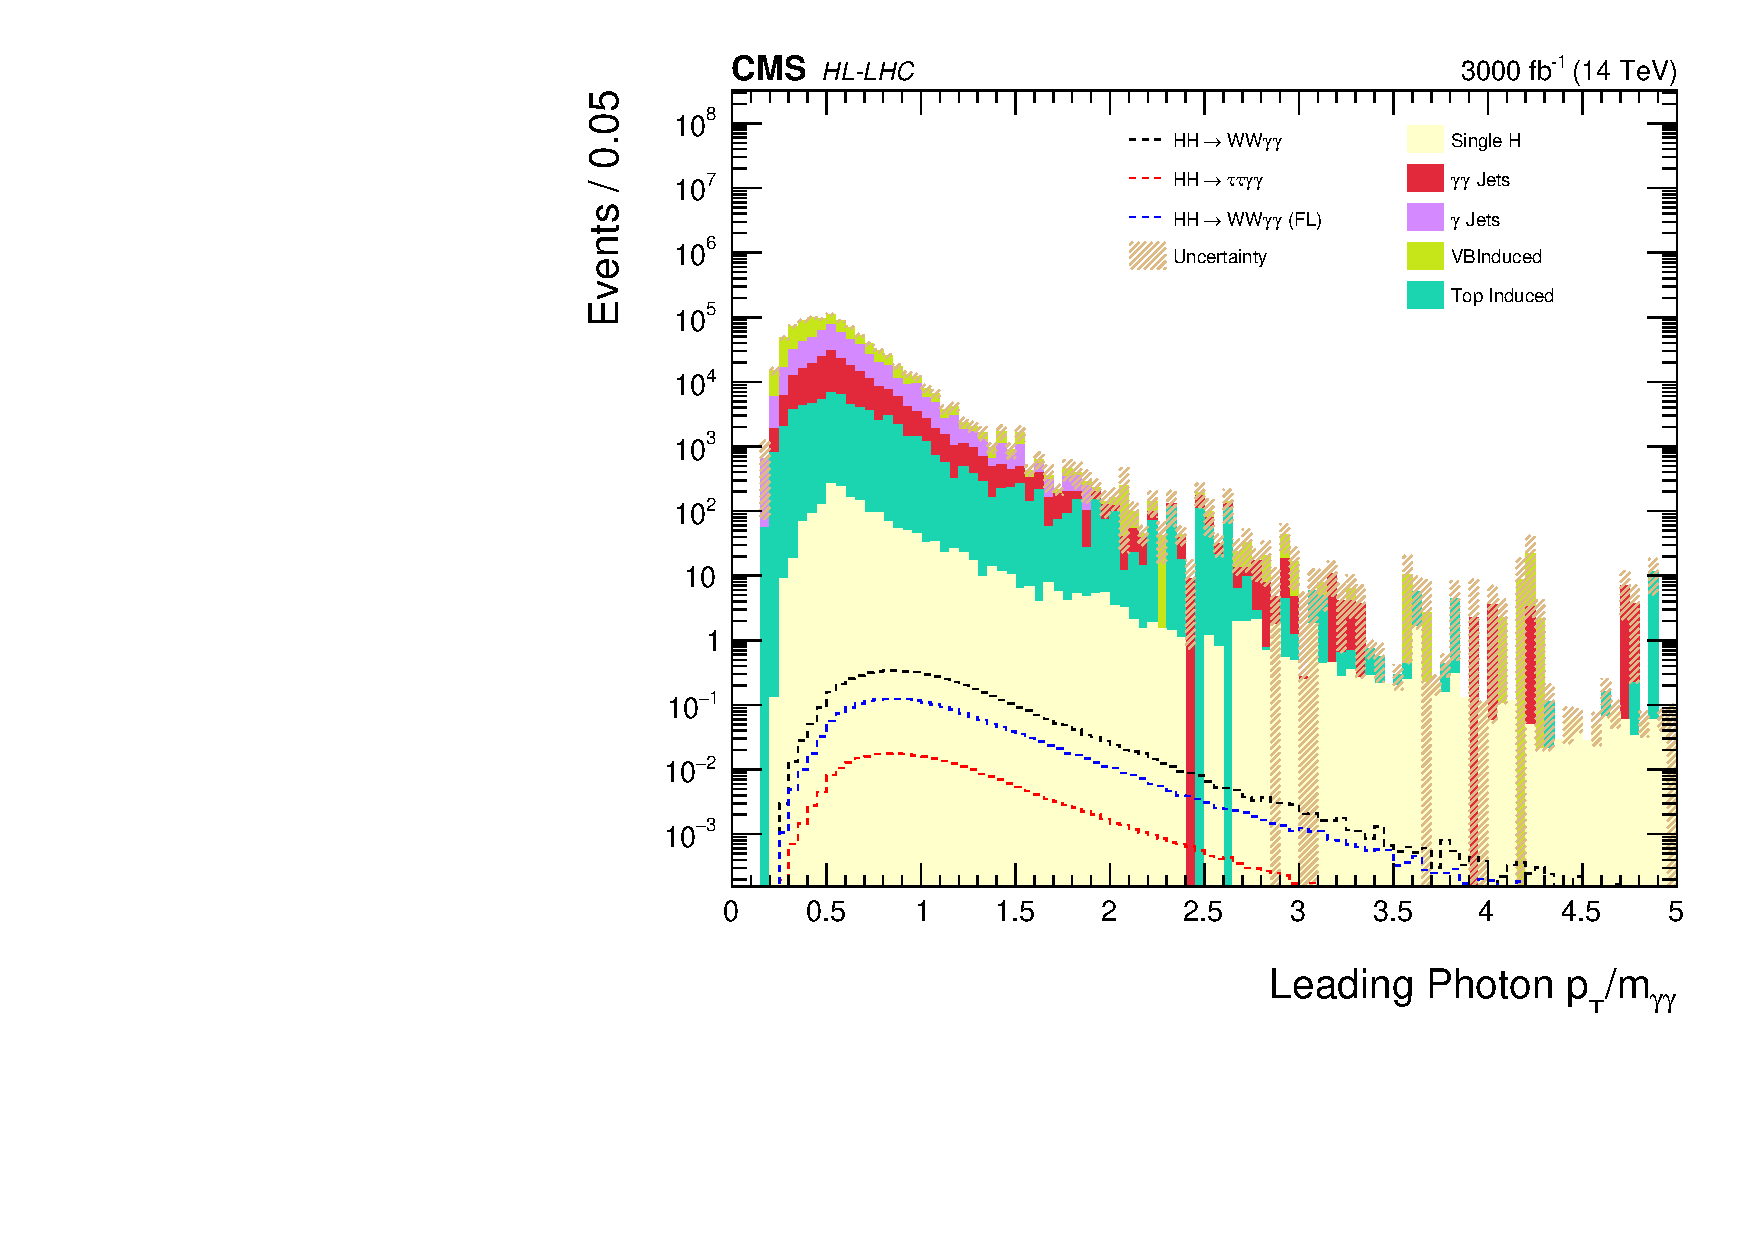
\includegraphics[width=\textwidth]{LeadingPhotonpT_mGGLhasOneL_logy.pdf}
        \vspace{-0.5cm}
        \firstsubcaption{Leading Photon p$_T$/\mgg}
    \end{subfigure}
    \hfill
    \begin{subfigure}[b]{0.475\textwidth}  
        \centering 
        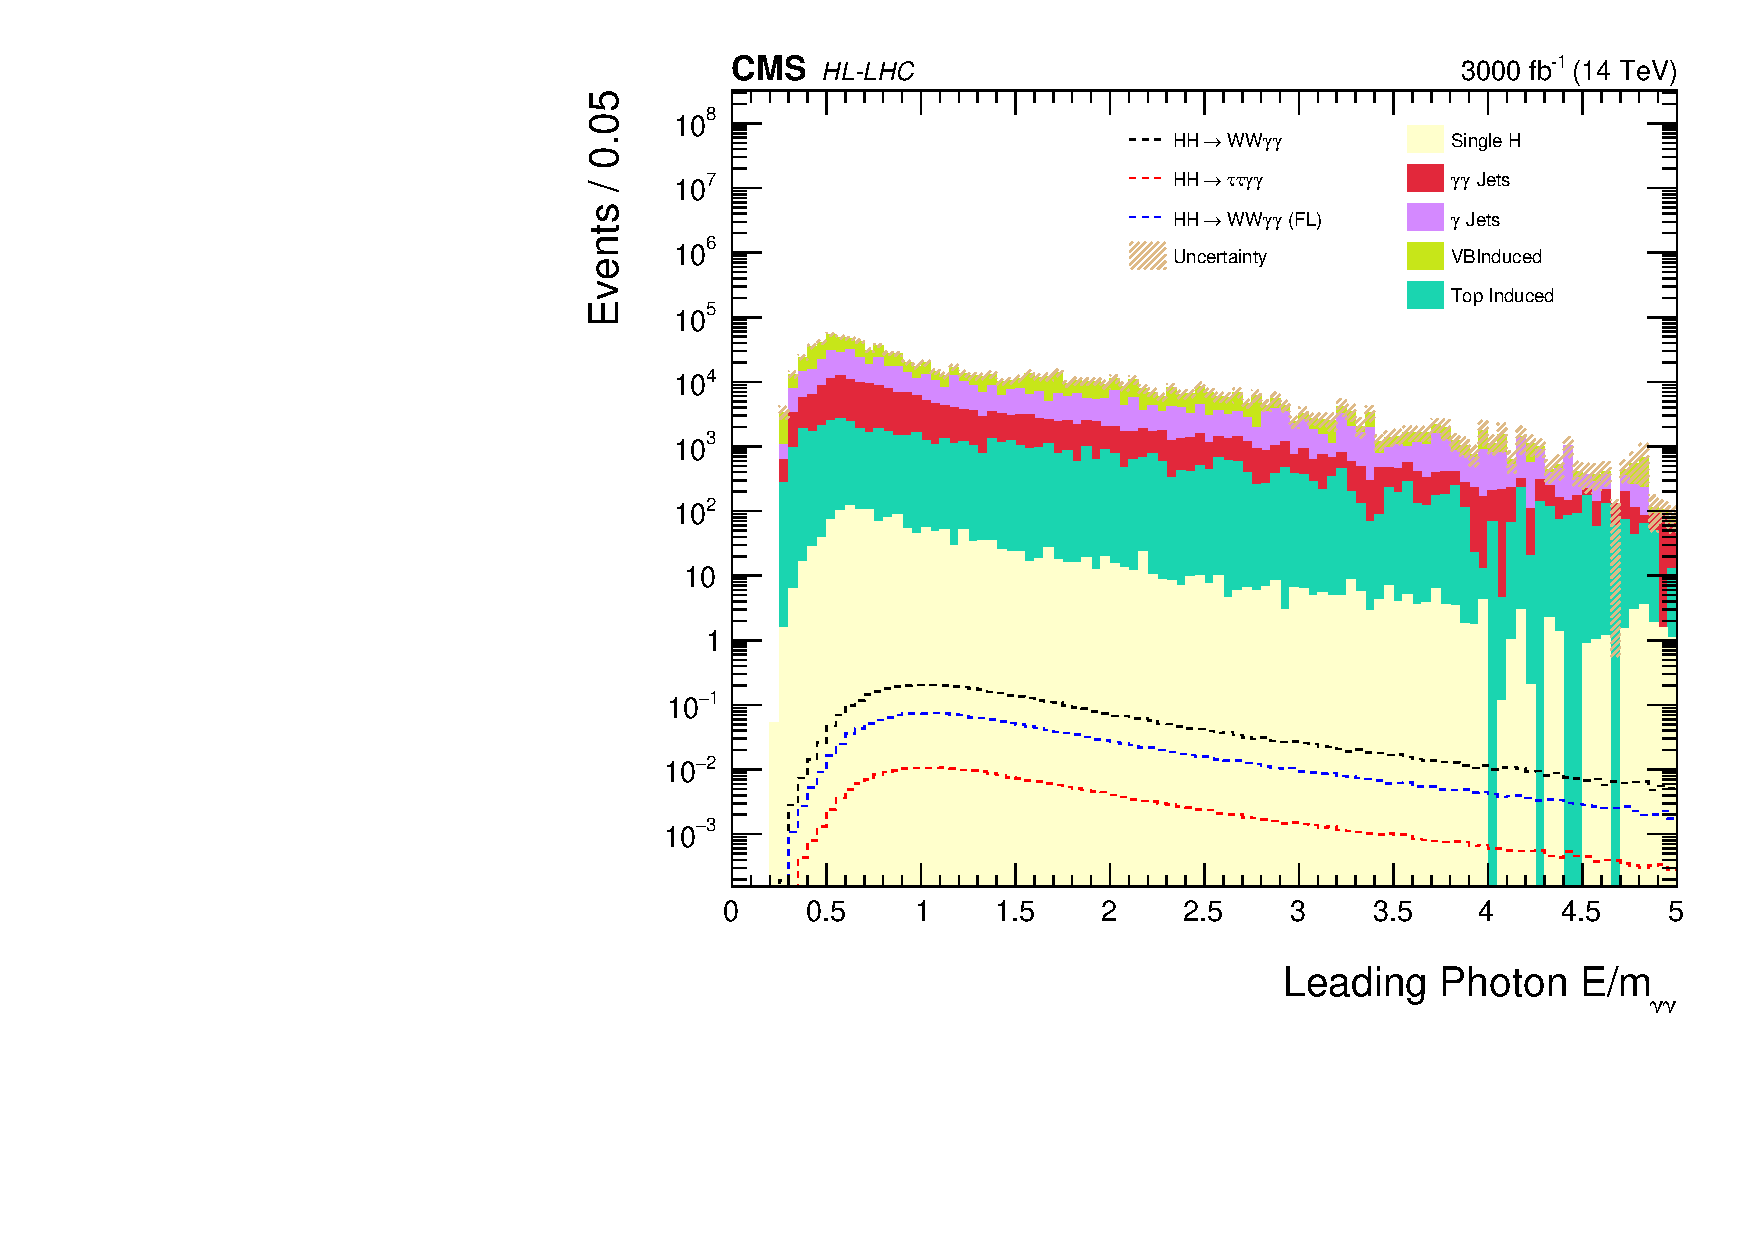
\includegraphics[width=\textwidth]{LeadingPhotonE_mGGLhasOneL_logy.pdf}
        \vspace{-0.5cm}
        \firstsubcaption{Leading Photon E/\mgg}
    \end{subfigure}
    \vskip\baselineskip
    \begin{subfigure}[b]{0.475\textwidth}   
        \centering 
        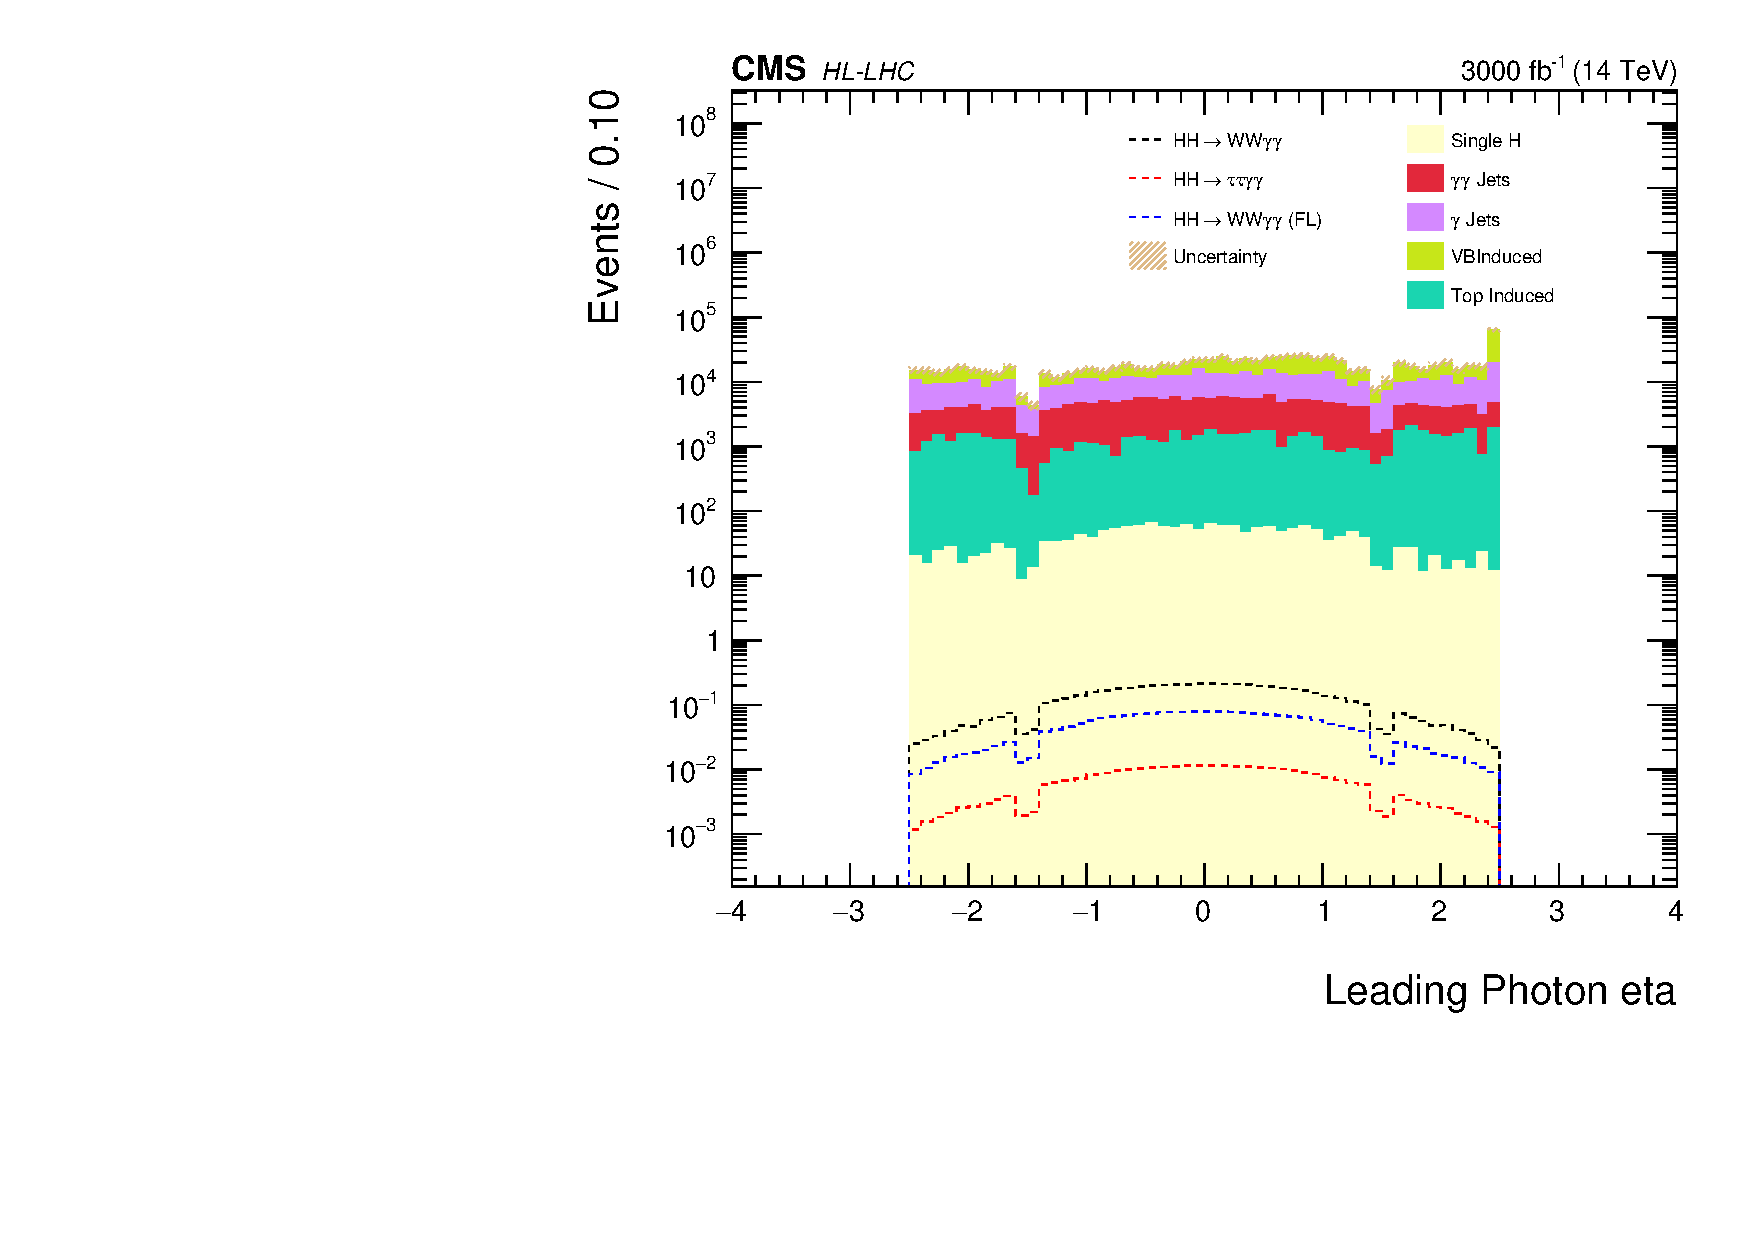
\includegraphics[width=\textwidth]{LeadingPhotonEtaOneL_logy.pdf}
        \vspace{-0.5cm}
        \firstsubcaption{Leading Photon $\eta$}
    \end{subfigure}
    \hfill
    \begin{subfigure}[b]{0.475\textwidth}   
        \centering 
        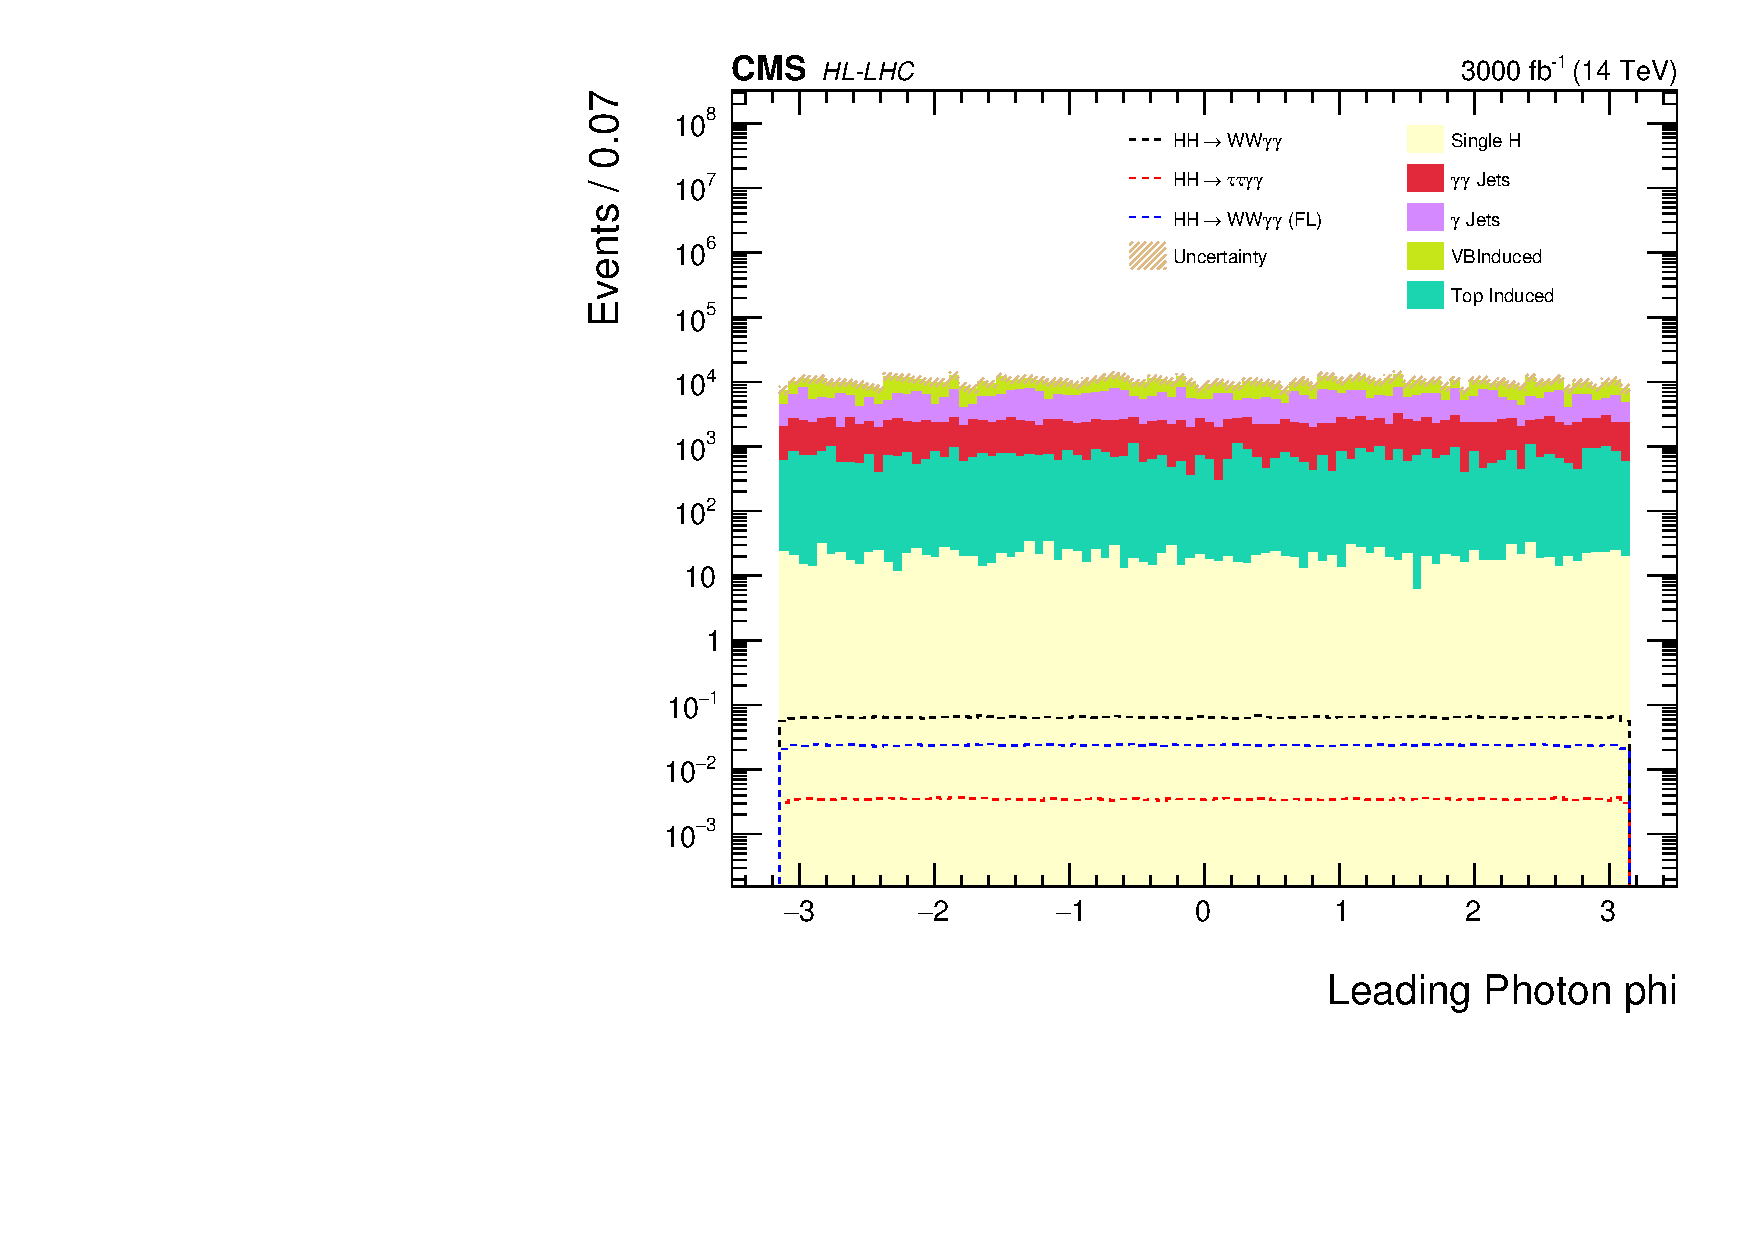
\includegraphics[width=\textwidth]{LeadingPhotonPhiOneL_logy.pdf}
        \vspace{-0.5cm}
        \firstsubcaption{Leading Photon $\phi$}
    \end{subfigure}
    \vskip\baselineskip
    \begin{subfigure}[b]{0.475\textwidth}   
        \centering 
        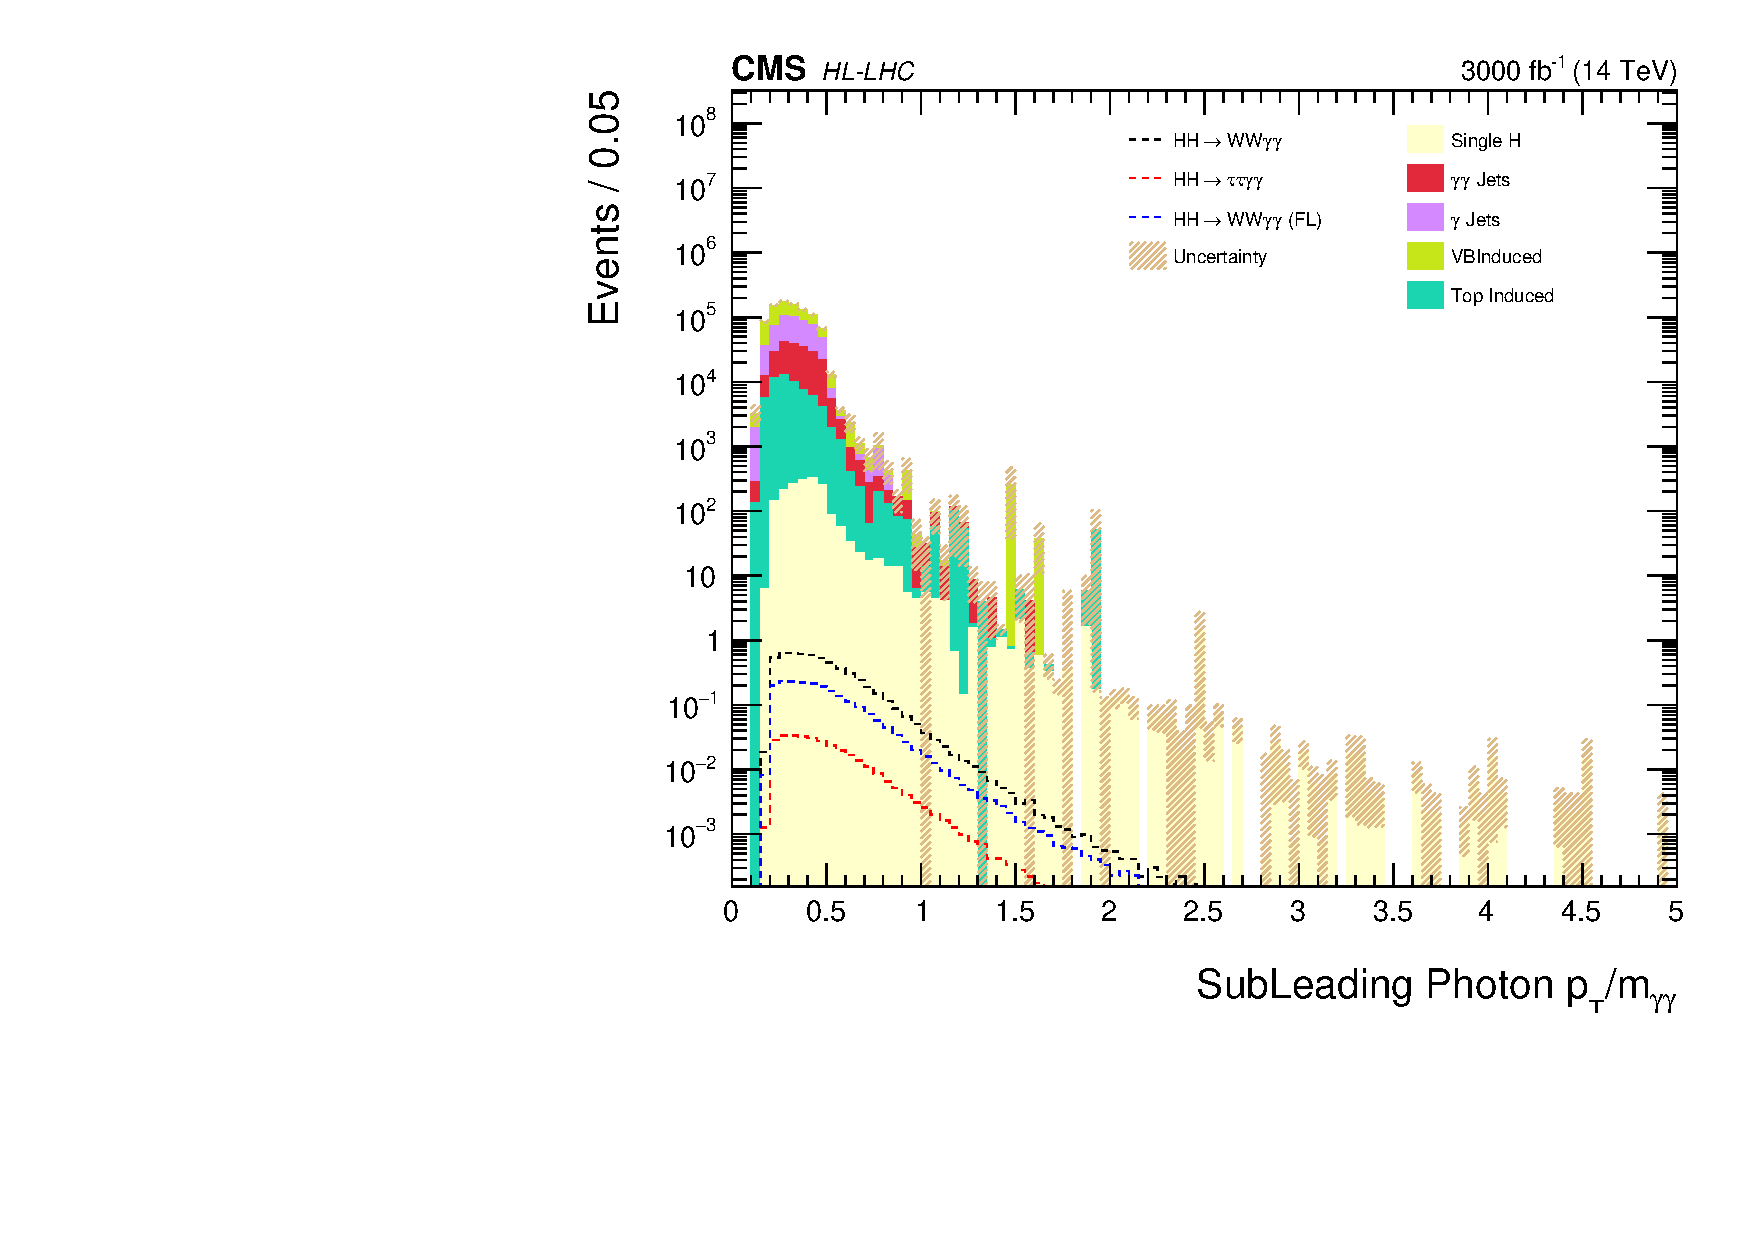
\includegraphics[width=\textwidth]{SubLeadingPhotonpT_mGGLhasOneL_logy.pdf}
        \vspace{-0.5cm}
        \firstsubcaption{Sub-leading Photon p$_T$/\mgg}
    \end{subfigure}
    \hfill
    \begin{subfigure}[b]{0.475\textwidth}   
        \centering 
        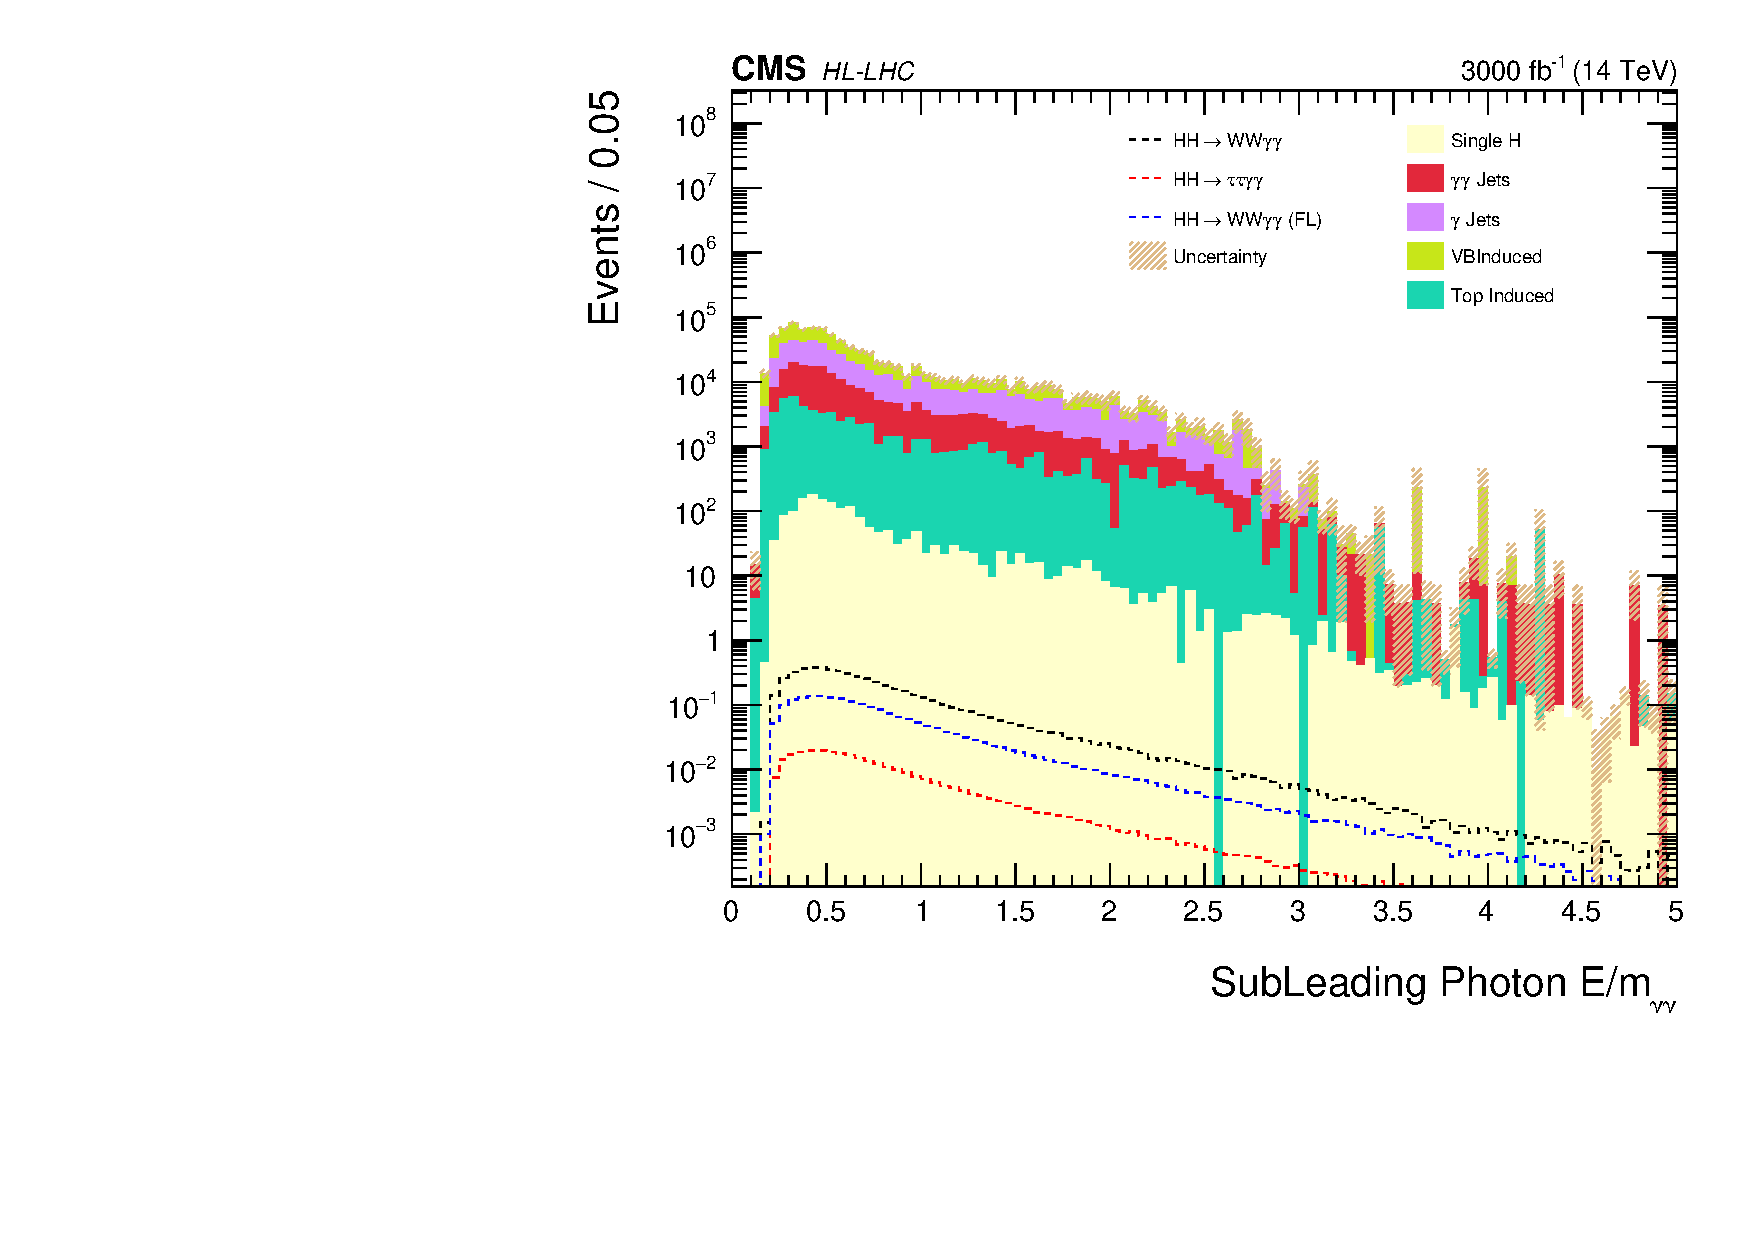
\includegraphics[width=\textwidth]{SubLeadingPhotonE_mGGLhasOneL_logy.pdf}
        \vspace{-0.5cm}
        \firstsubcaption{Sub-leading Photon E/\mgg}   
    \end{subfigure}
    \caption{\small DNN input distributions for the semi-leptonic channel of $HH\rightarrow{WW\gamma\gamma}$.} 
    \label{hasOneL_plots}
\end{figure*}

\begin{figure*}[h!]
    \centering
    \begin{subfigure}[b]{0.475\textwidth}
        \centering
        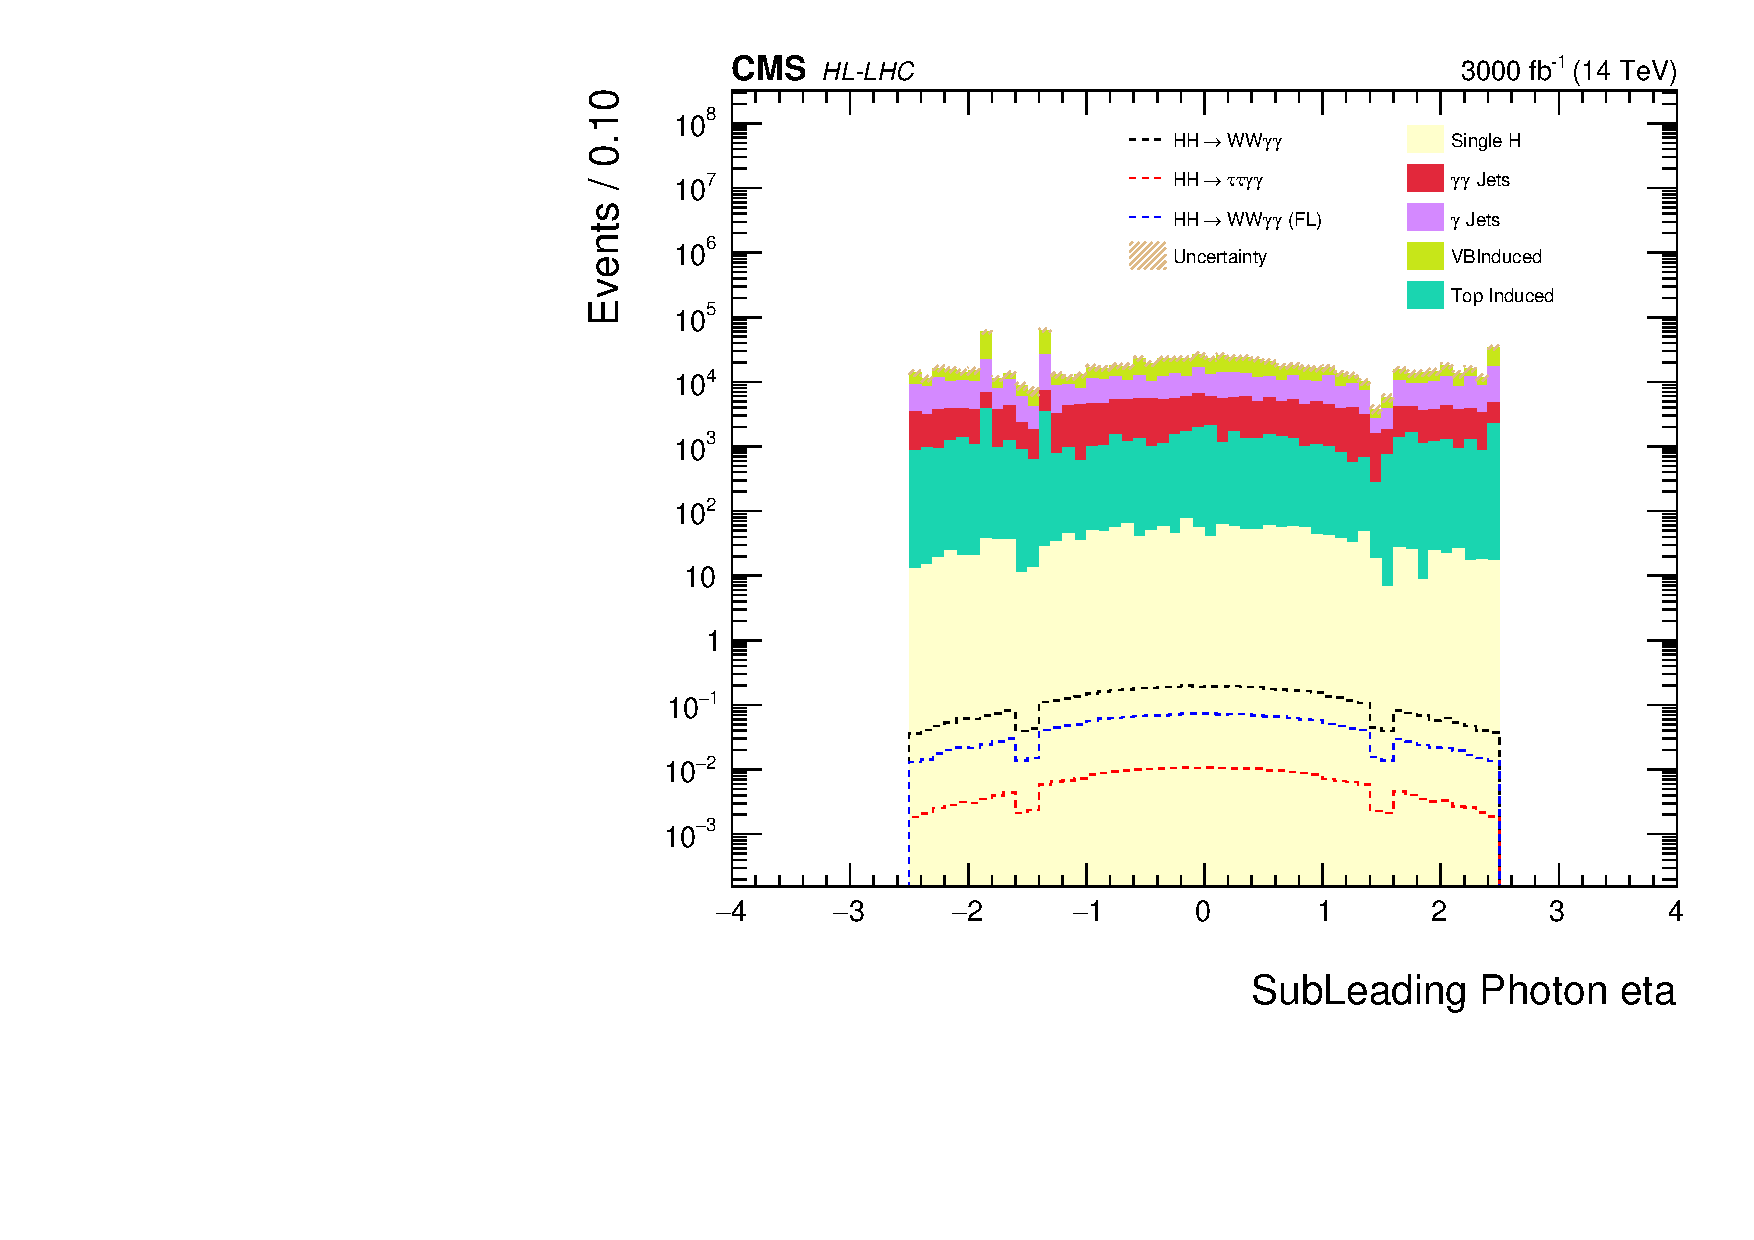
\includegraphics[width=\textwidth]{SubLeadingPhotonEtaOneL_logy.pdf}
        \vspace{-0.5cm}
        \firstsubcaption{Sub-leading Photon $\eta$}
    \end{subfigure}
    \hfill
    \begin{subfigure}[b]{0.475\textwidth}  
        \centering 
        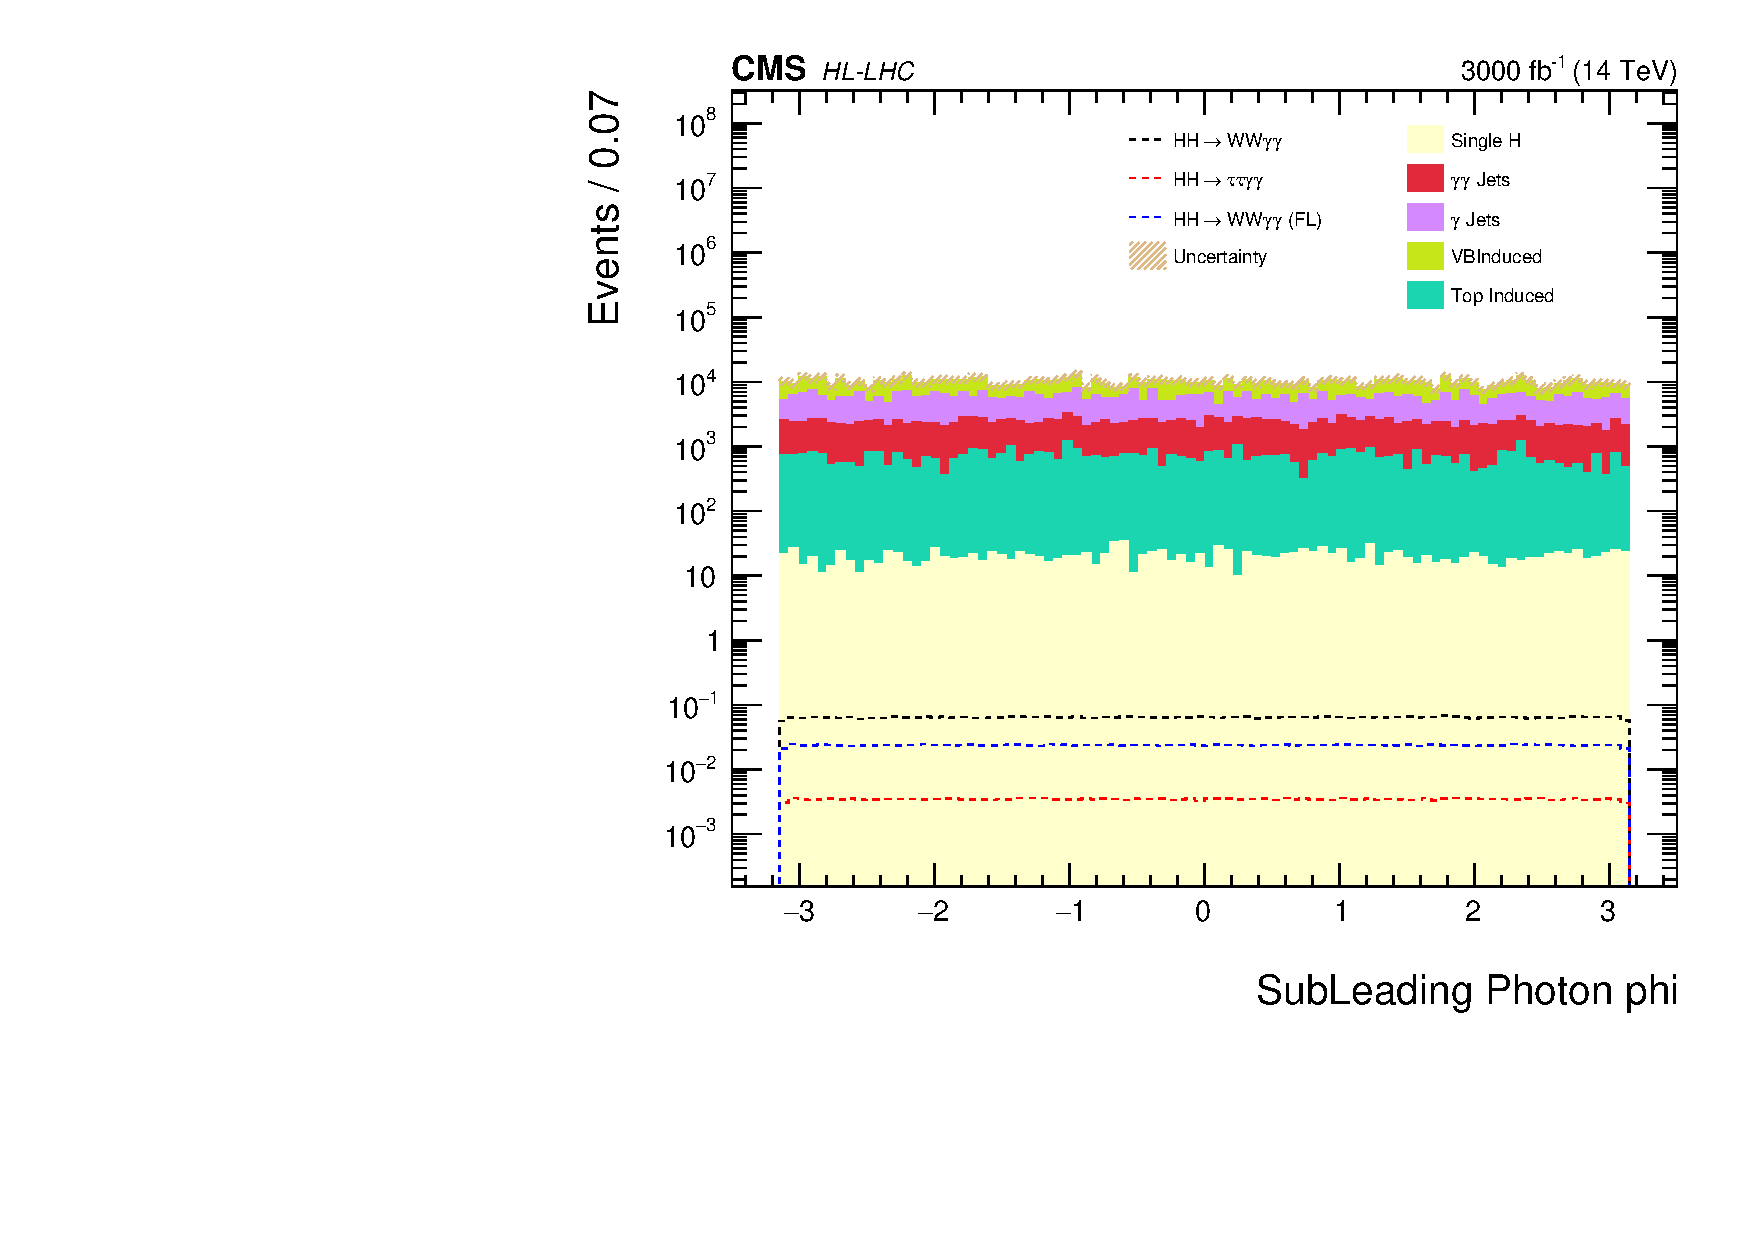
\includegraphics[width=\textwidth]{SubLeadingPhotonPhiOneL_logy.pdf}
        \vspace{-0.5cm}
        \firstsubcaption{Sub-leading Photon $\phi$}
    \end{subfigure}
    \vskip\baselineskip
    \begin{subfigure}[b]{0.475\textwidth}   
        \centering 
        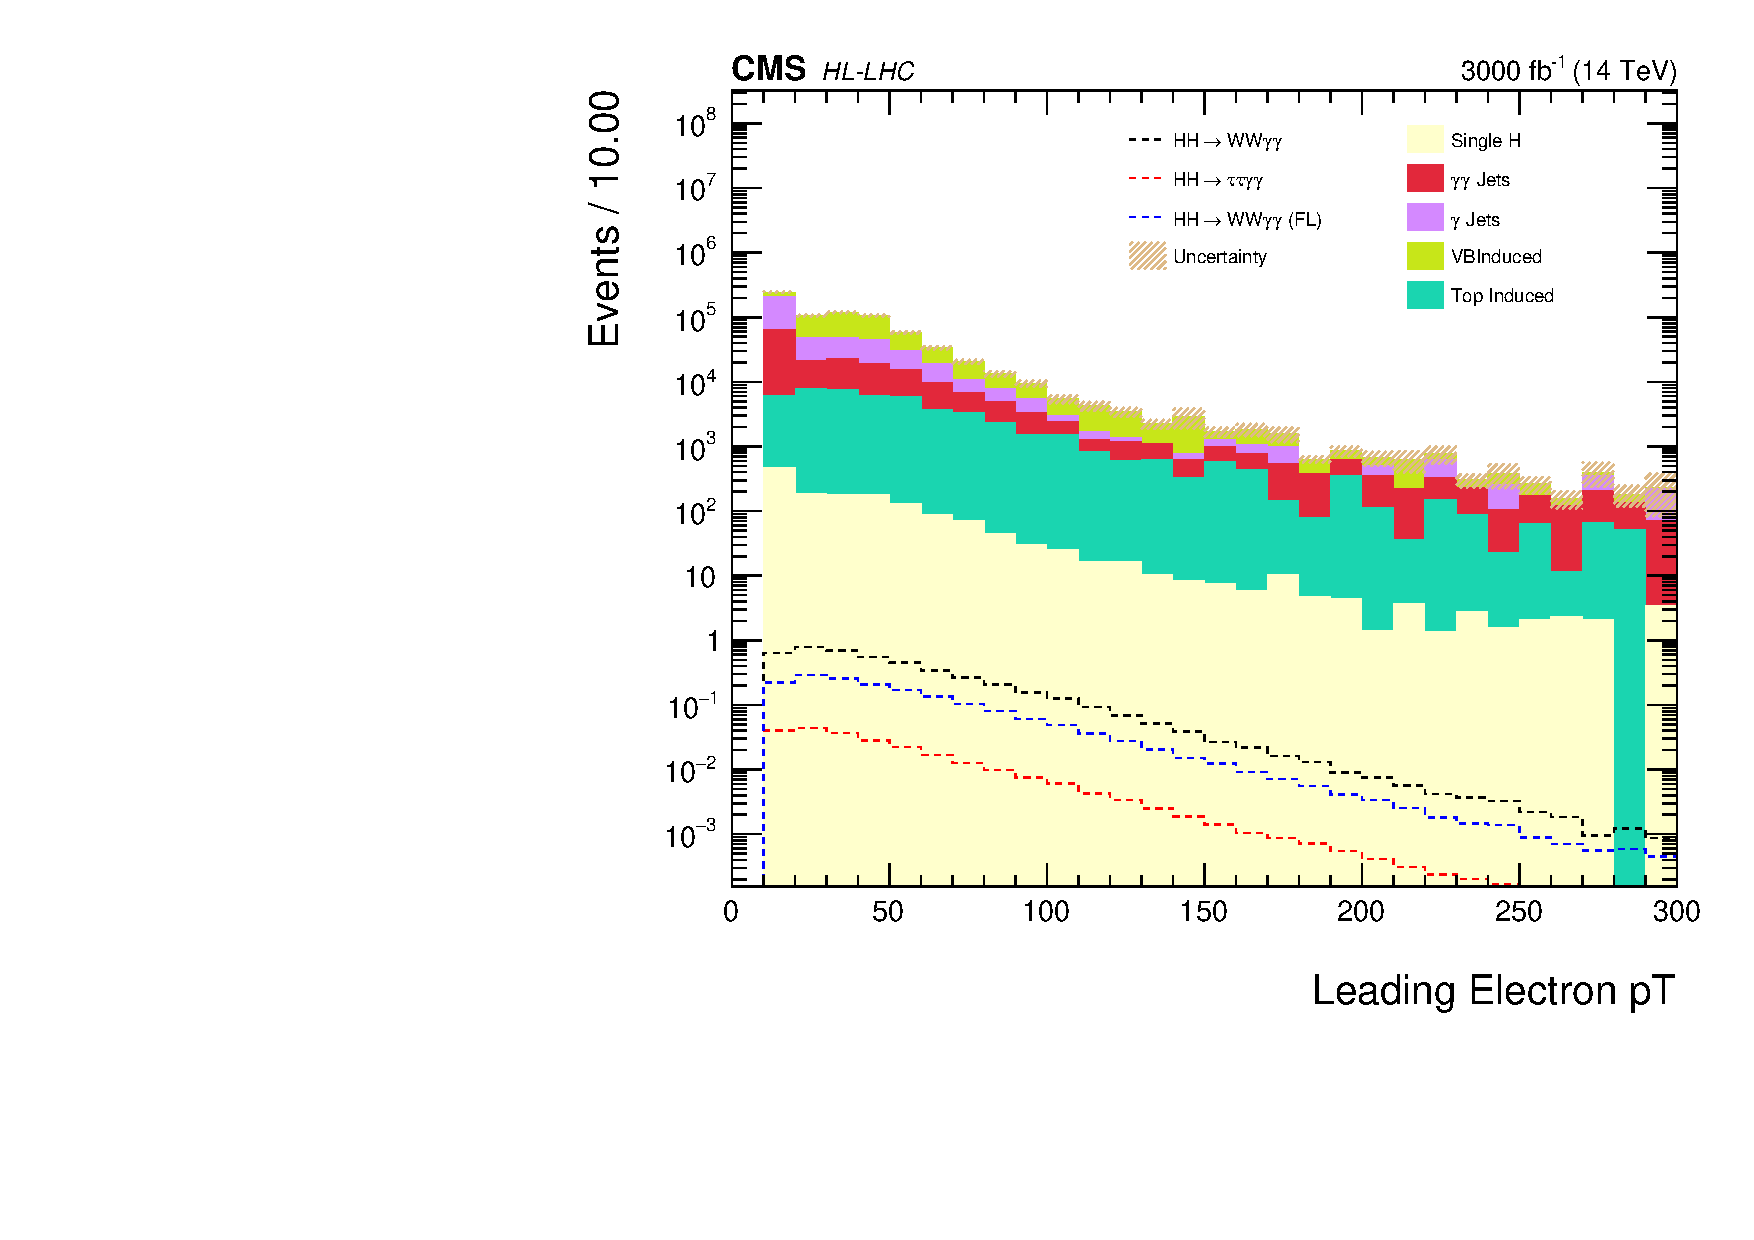
\includegraphics[width=\textwidth]{ElectronpT_logy.pdf}
        \vspace{-0.5cm}
        \firstsubcaption{Electron p$_{T}$}
    \end{subfigure}
    \hfill
    \begin{subfigure}[b]{0.475\textwidth}   
        \centering 
        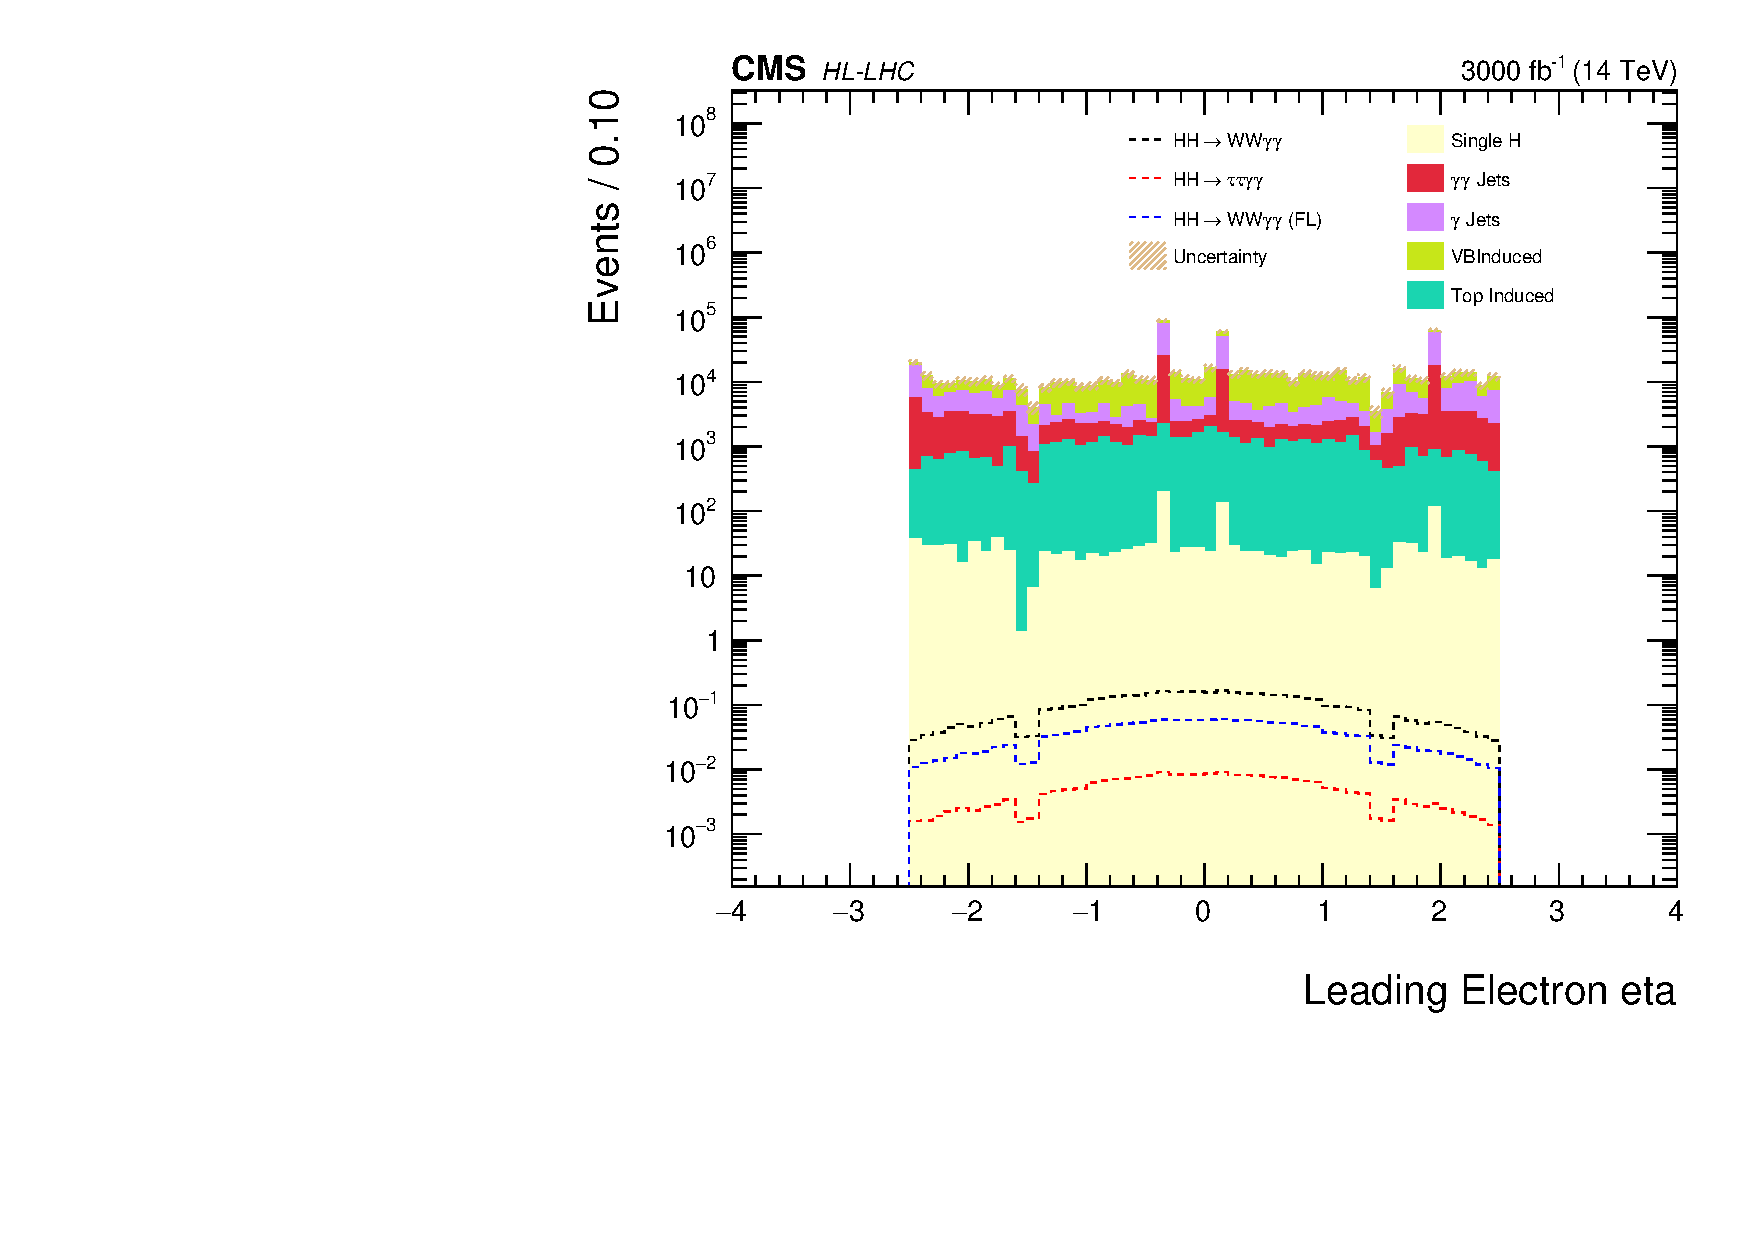
\includegraphics[width=\textwidth]{ElectronEta_logy.pdf}
        \vspace{-0.5cm}
        \firstsubcaption{Electron $\eta$}
    \end{subfigure}
    \vskip\baselineskip
    \begin{subfigure}[b]{0.475\textwidth}   
        \centering 
        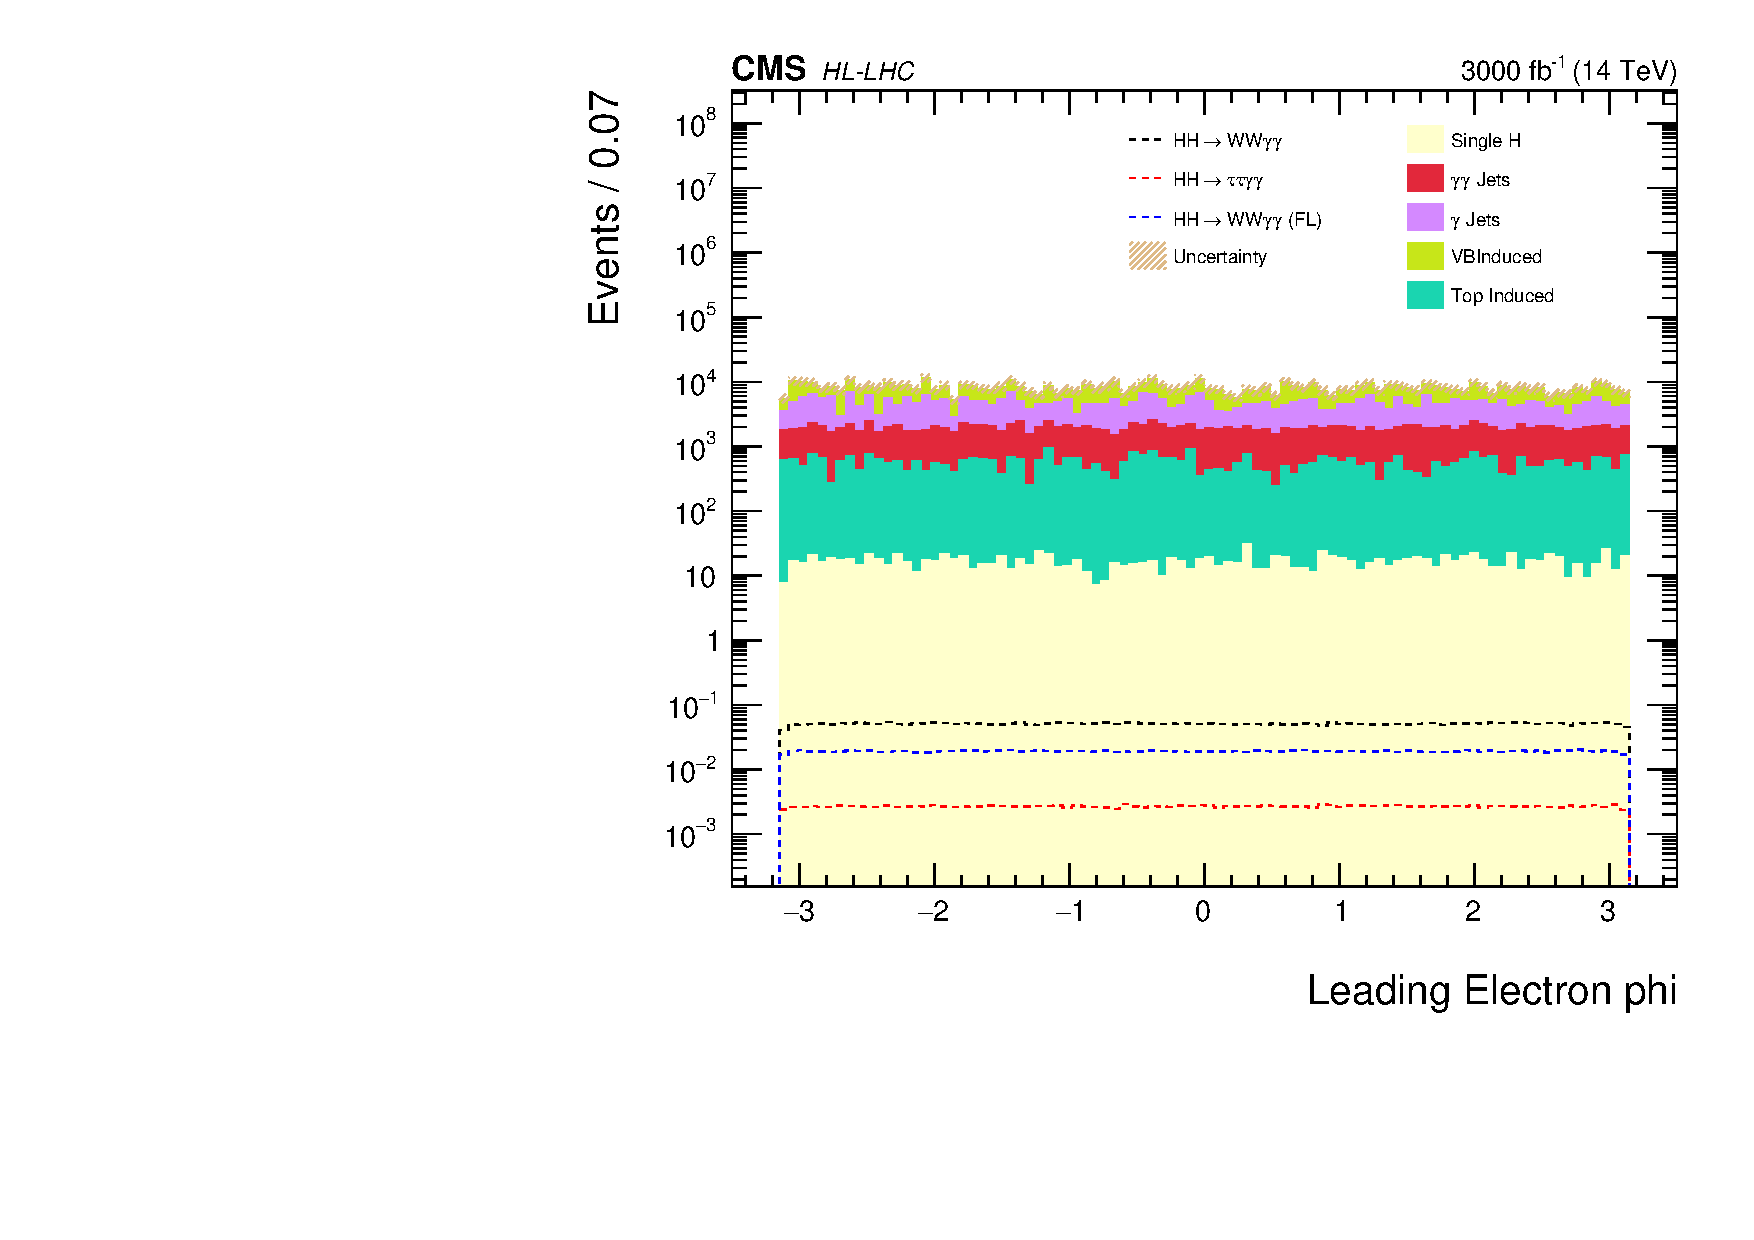
\includegraphics[width=\textwidth]{ElectronPhi_logy.pdf}
        \vspace{-0.5cm}
        \firstsubcaption{Electron $\phi$}
    \end{subfigure}
    \hfill
    \begin{subfigure}[b]{0.475\textwidth}   
        \centering 
        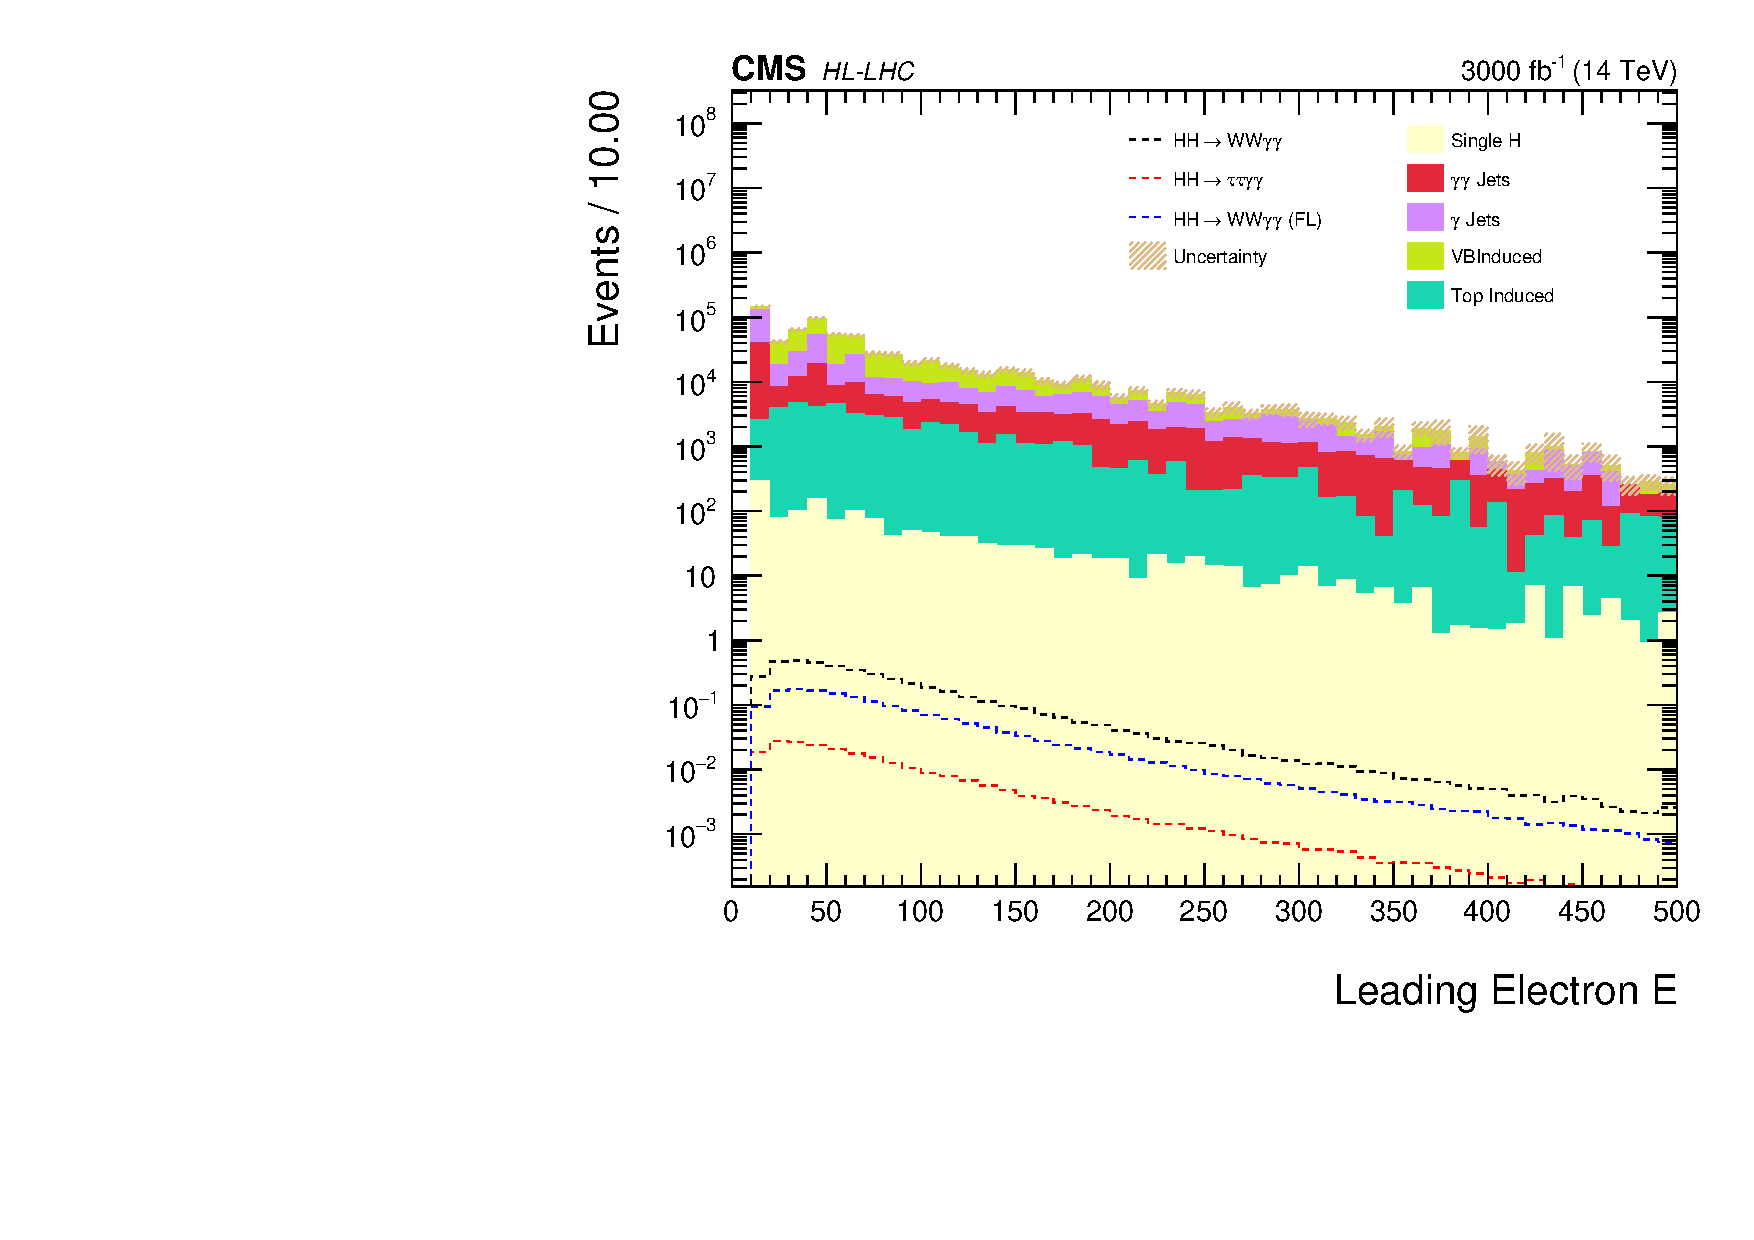
\includegraphics[width=\textwidth]{ElectronE_logy.pdf}
        \vspace{-0.5cm}
        \firstsubcaption{Electron energy}   
    \end{subfigure}
    \caption{\small DNN input distributions for the semi-leptonic channel of $HH\rightarrow{WW\gamma\gamma}$ (continued).}
\end{figure*}

\begin{figure*}[h!]
    \centering
    \begin{subfigure}[b]{0.475\textwidth}
        \centering
        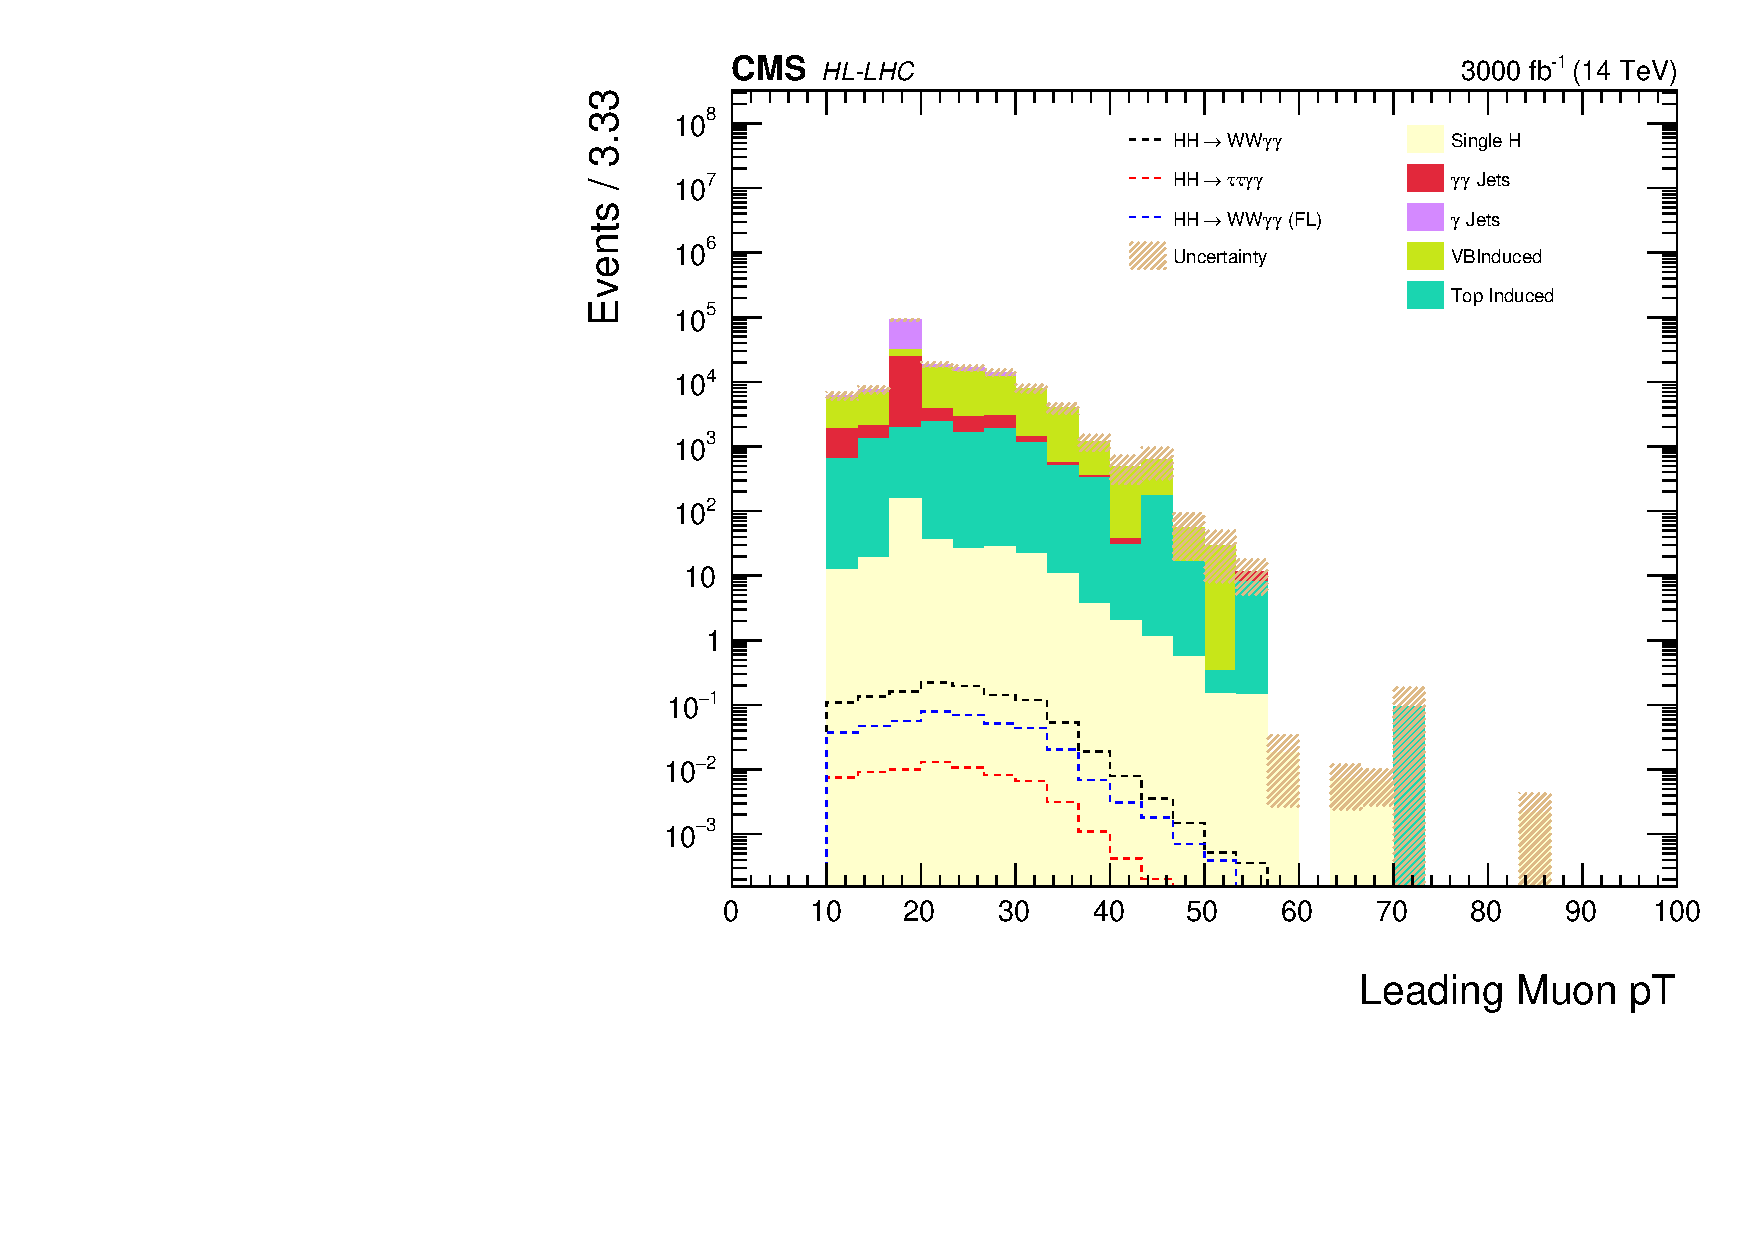
\includegraphics[width=\textwidth]{MuonpT_logy.pdf}
        \vspace{-0.5cm}
        \firstsubcaption{Muon \pt}
    \end{subfigure}
    \hfill
    \begin{subfigure}[b]{0.475\textwidth}  
        \centering 
        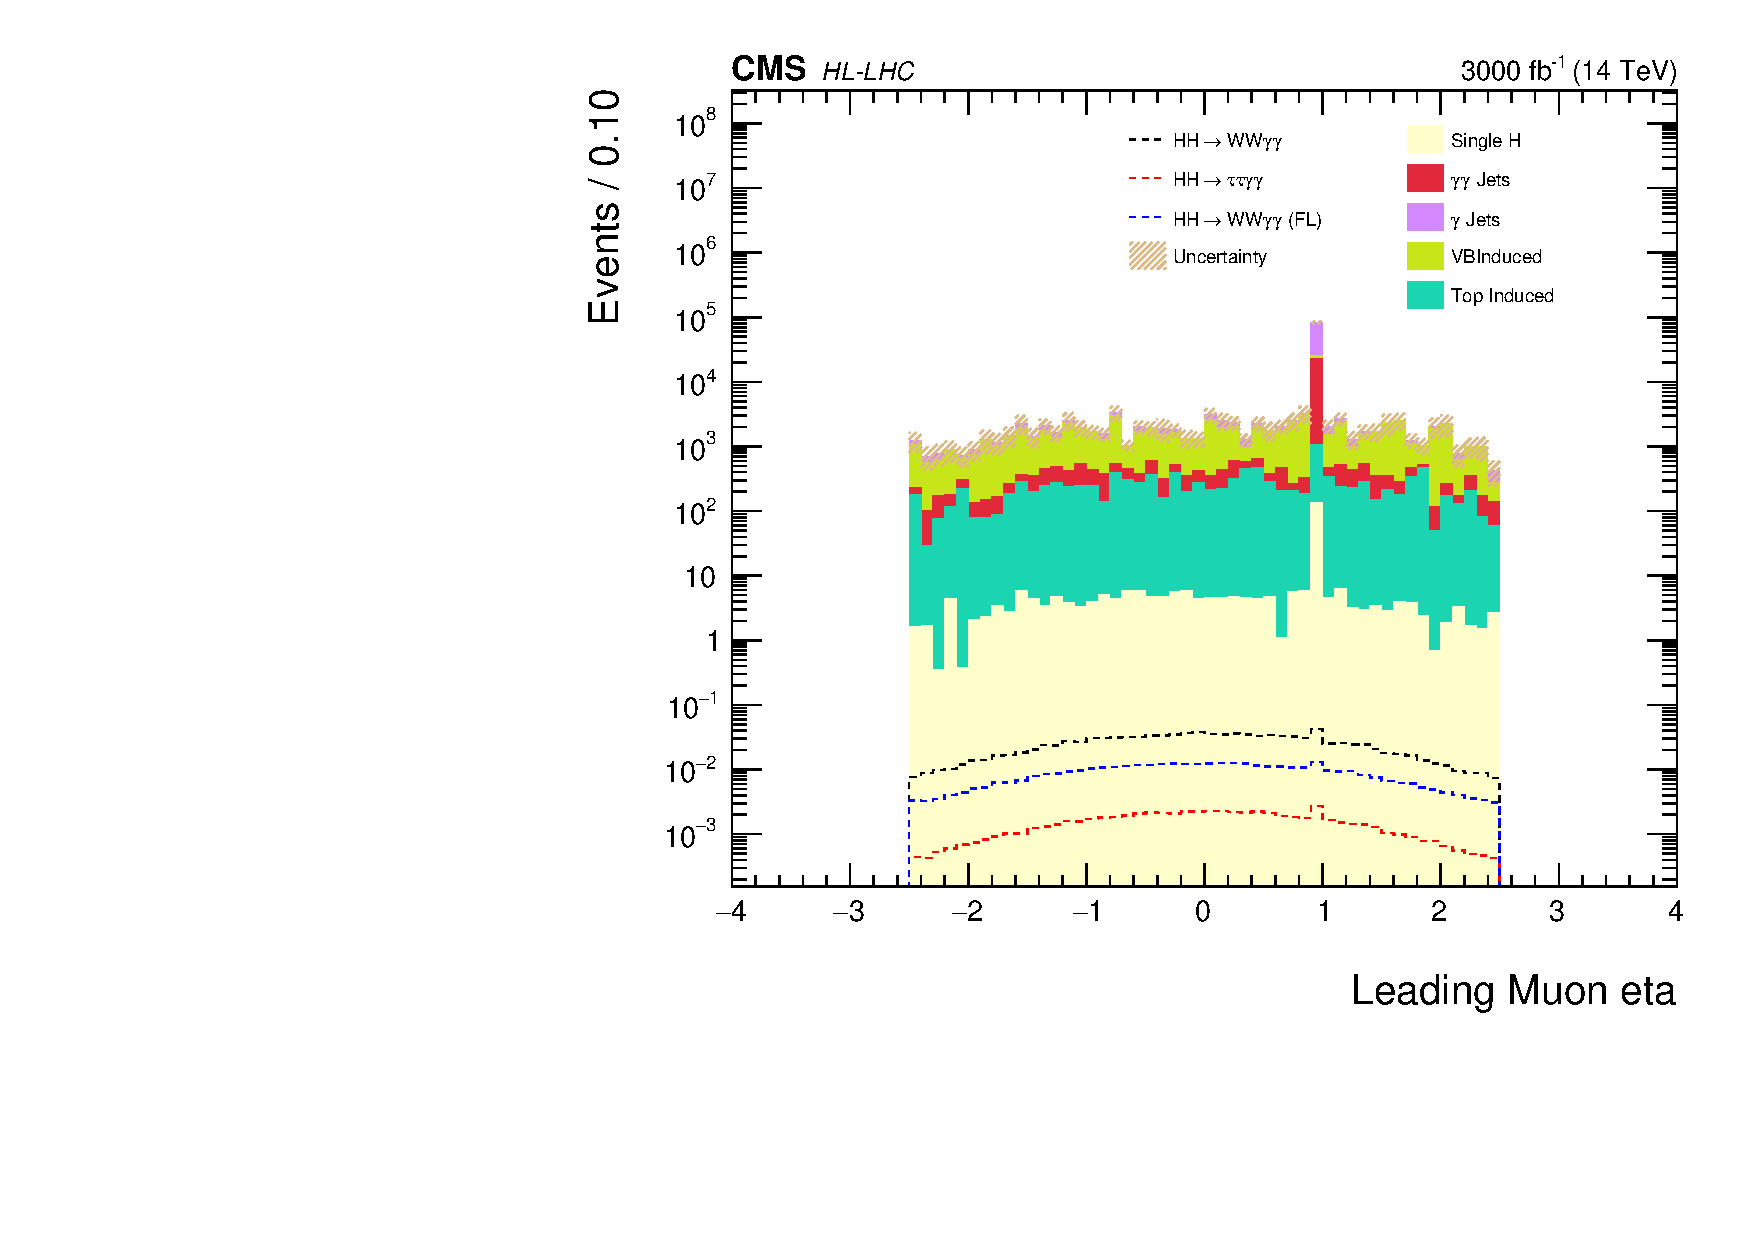
\includegraphics[width=\textwidth]{MuonEta_logy.pdf}
        \vspace{-0.5cm}
        \firstsubcaption{Muon $\eta$}
    \end{subfigure}
    \vskip\baselineskip
    \begin{subfigure}[b]{0.475\textwidth}   
        \centering 
        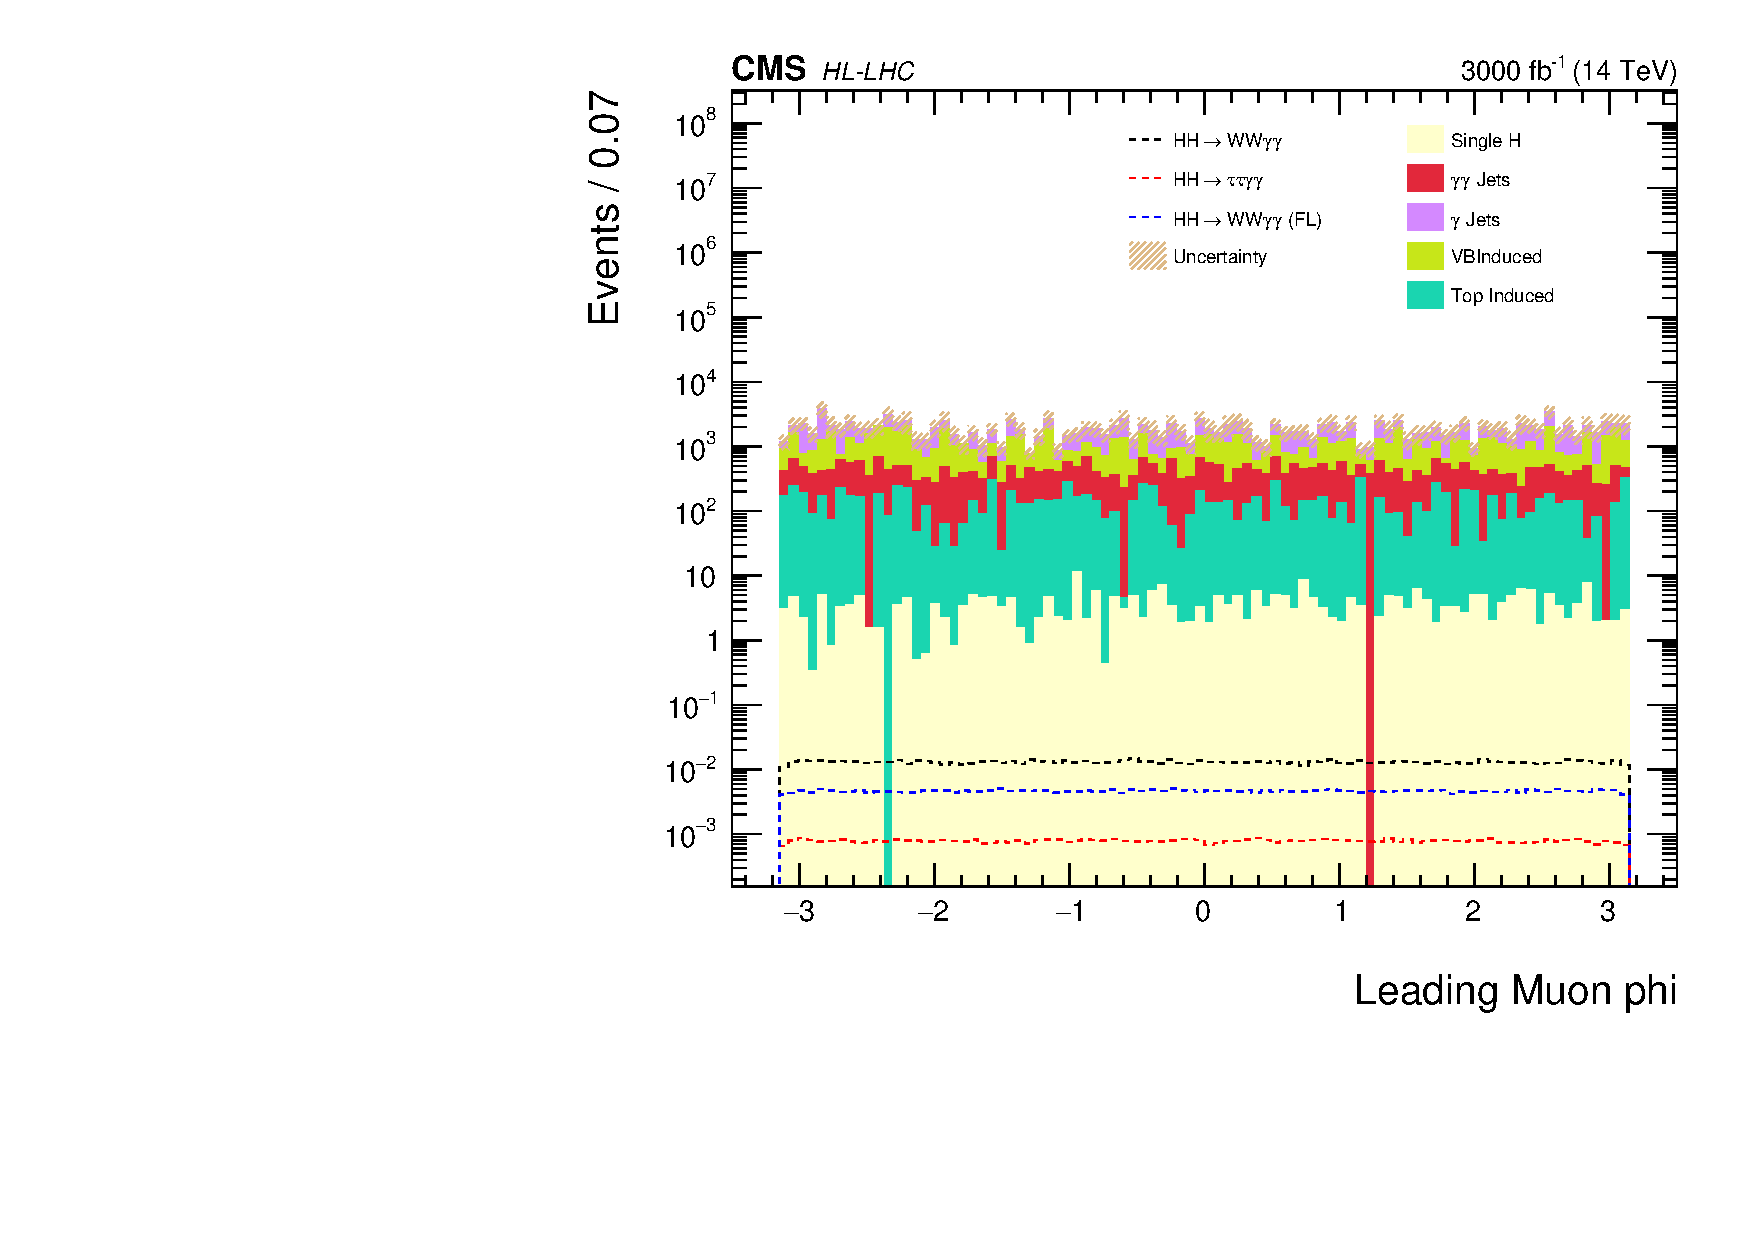
\includegraphics[width=\textwidth]{MuonPhi_logy.pdf}
        \vspace{-0.5cm}
        \firstsubcaption{Muon $\phi$}
    \end{subfigure}
    \hfill
    \begin{subfigure}[b]{0.475\textwidth}   
        \centering 
        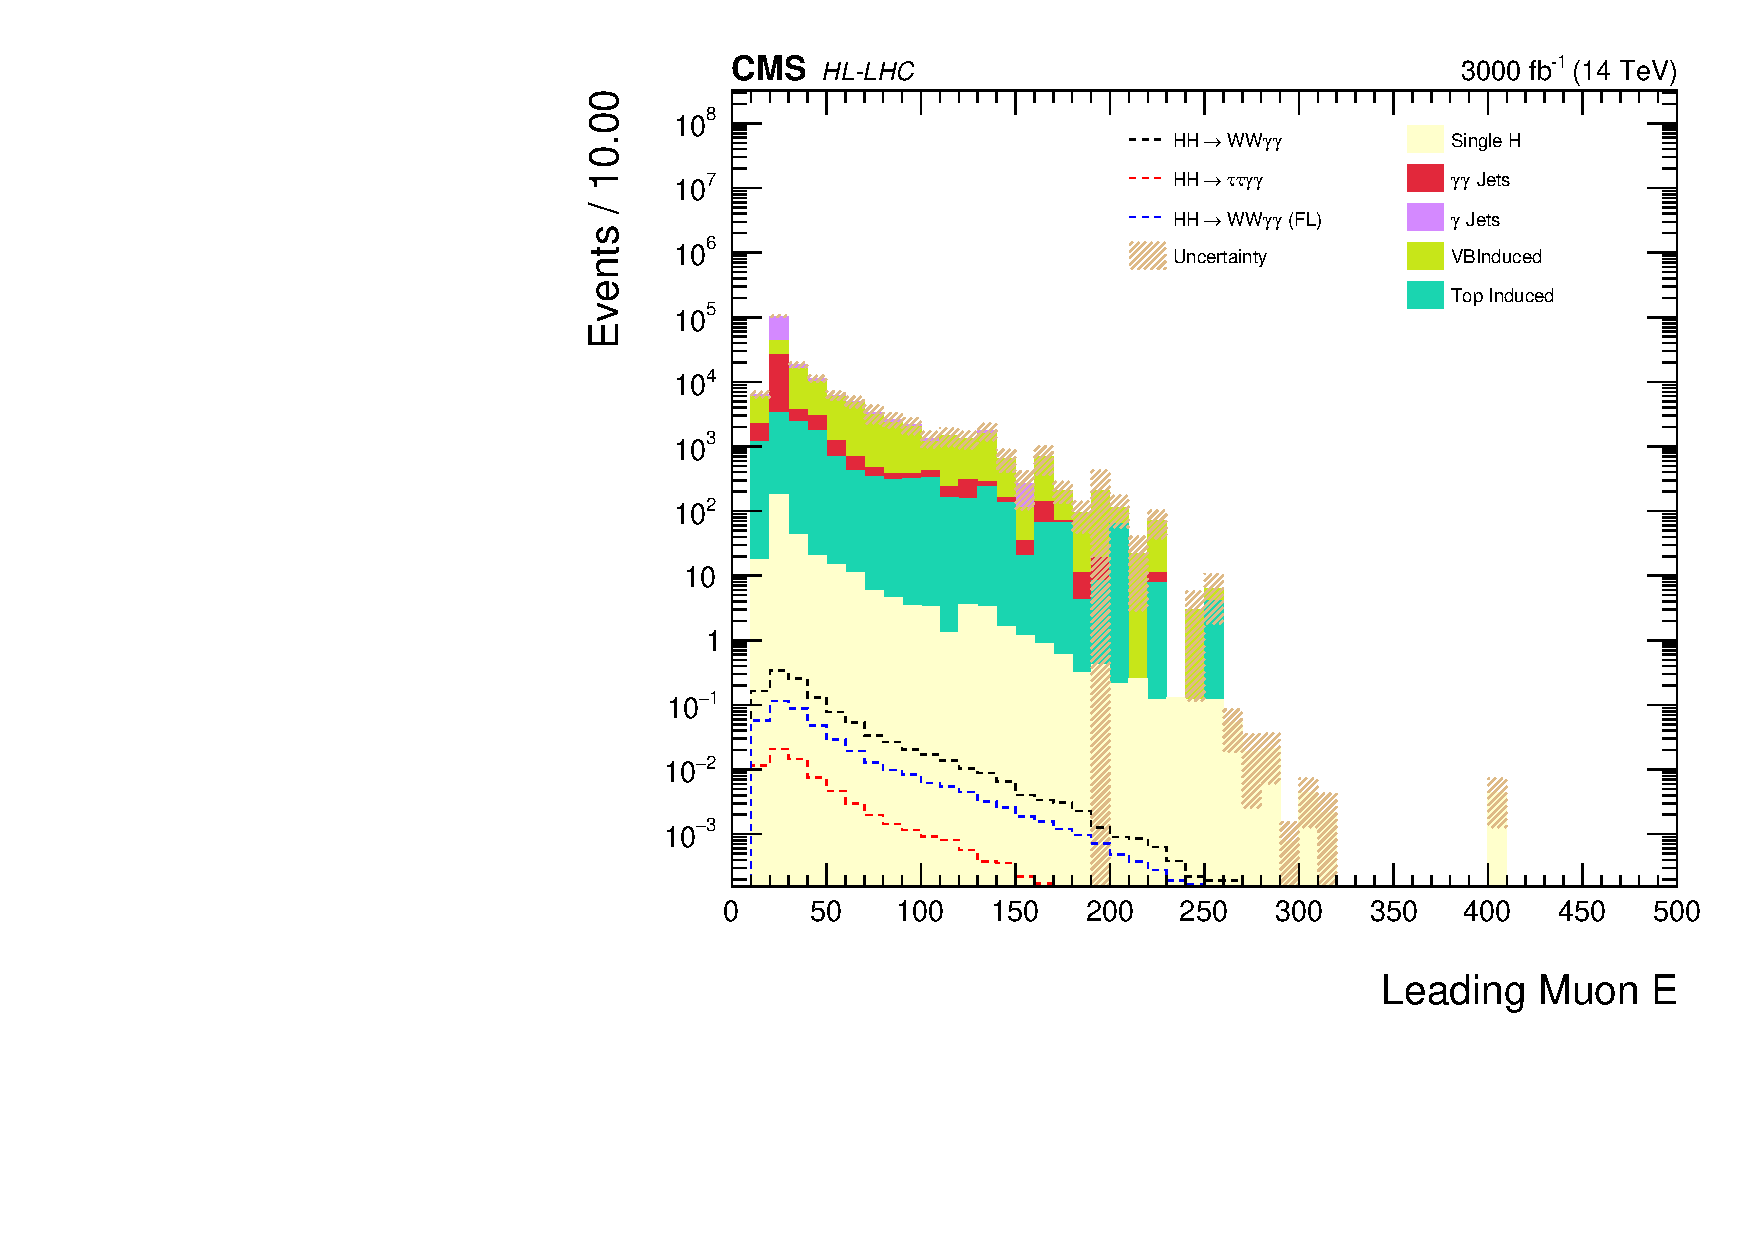
\includegraphics[width=\textwidth]{MuonE_logy.pdf}
        \vspace{-0.5cm}
        \firstsubcaption{Muon energy}
    \end{subfigure}
    \vskip\baselineskip
    \begin{subfigure}[b]{0.475\textwidth}   
        \centering 
        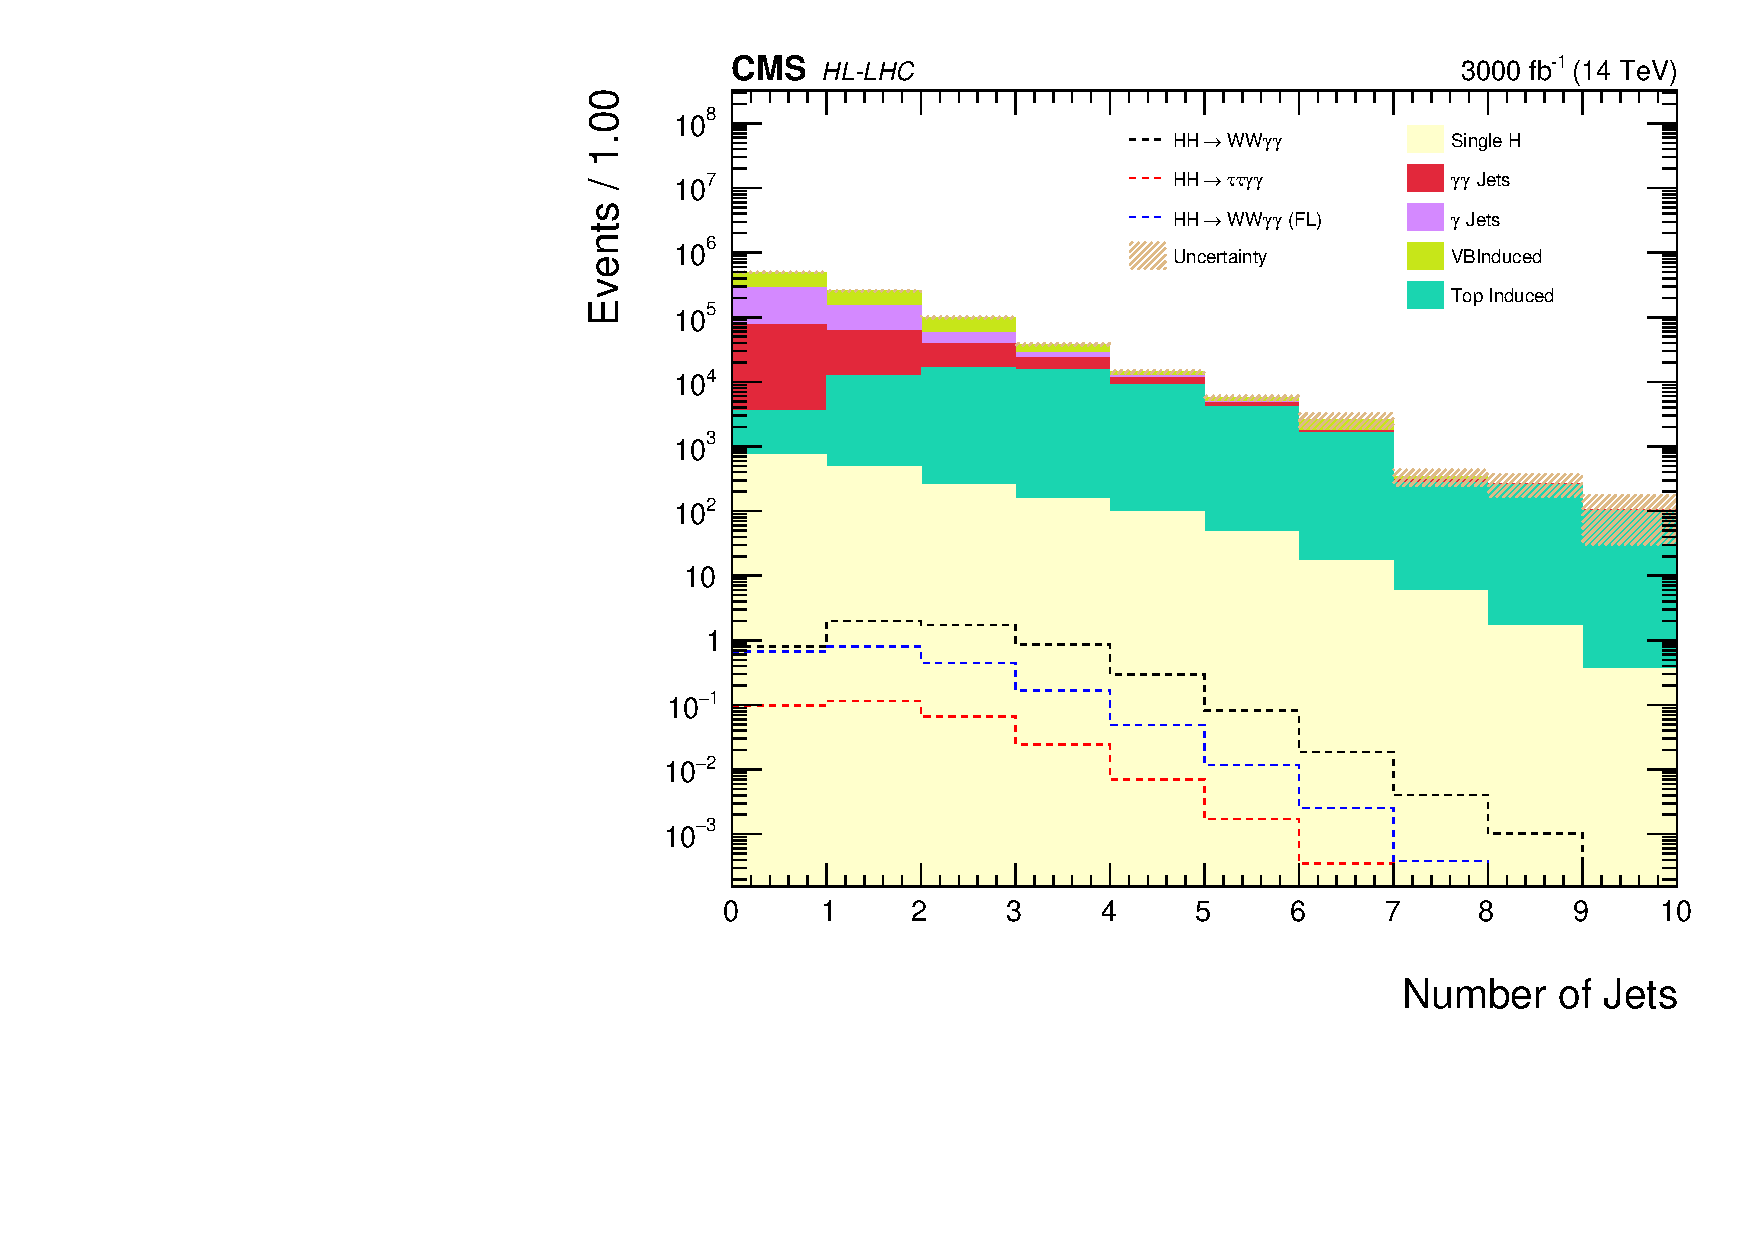
\includegraphics[width=\textwidth]{nJetsOneL_logy.pdf}
        \vspace{-0.5cm}
        \firstsubcaption{Jet multiplicity}
    \end{subfigure}
    \hfill
    \begin{subfigure}[b]{0.475\textwidth}   
        \centering 
        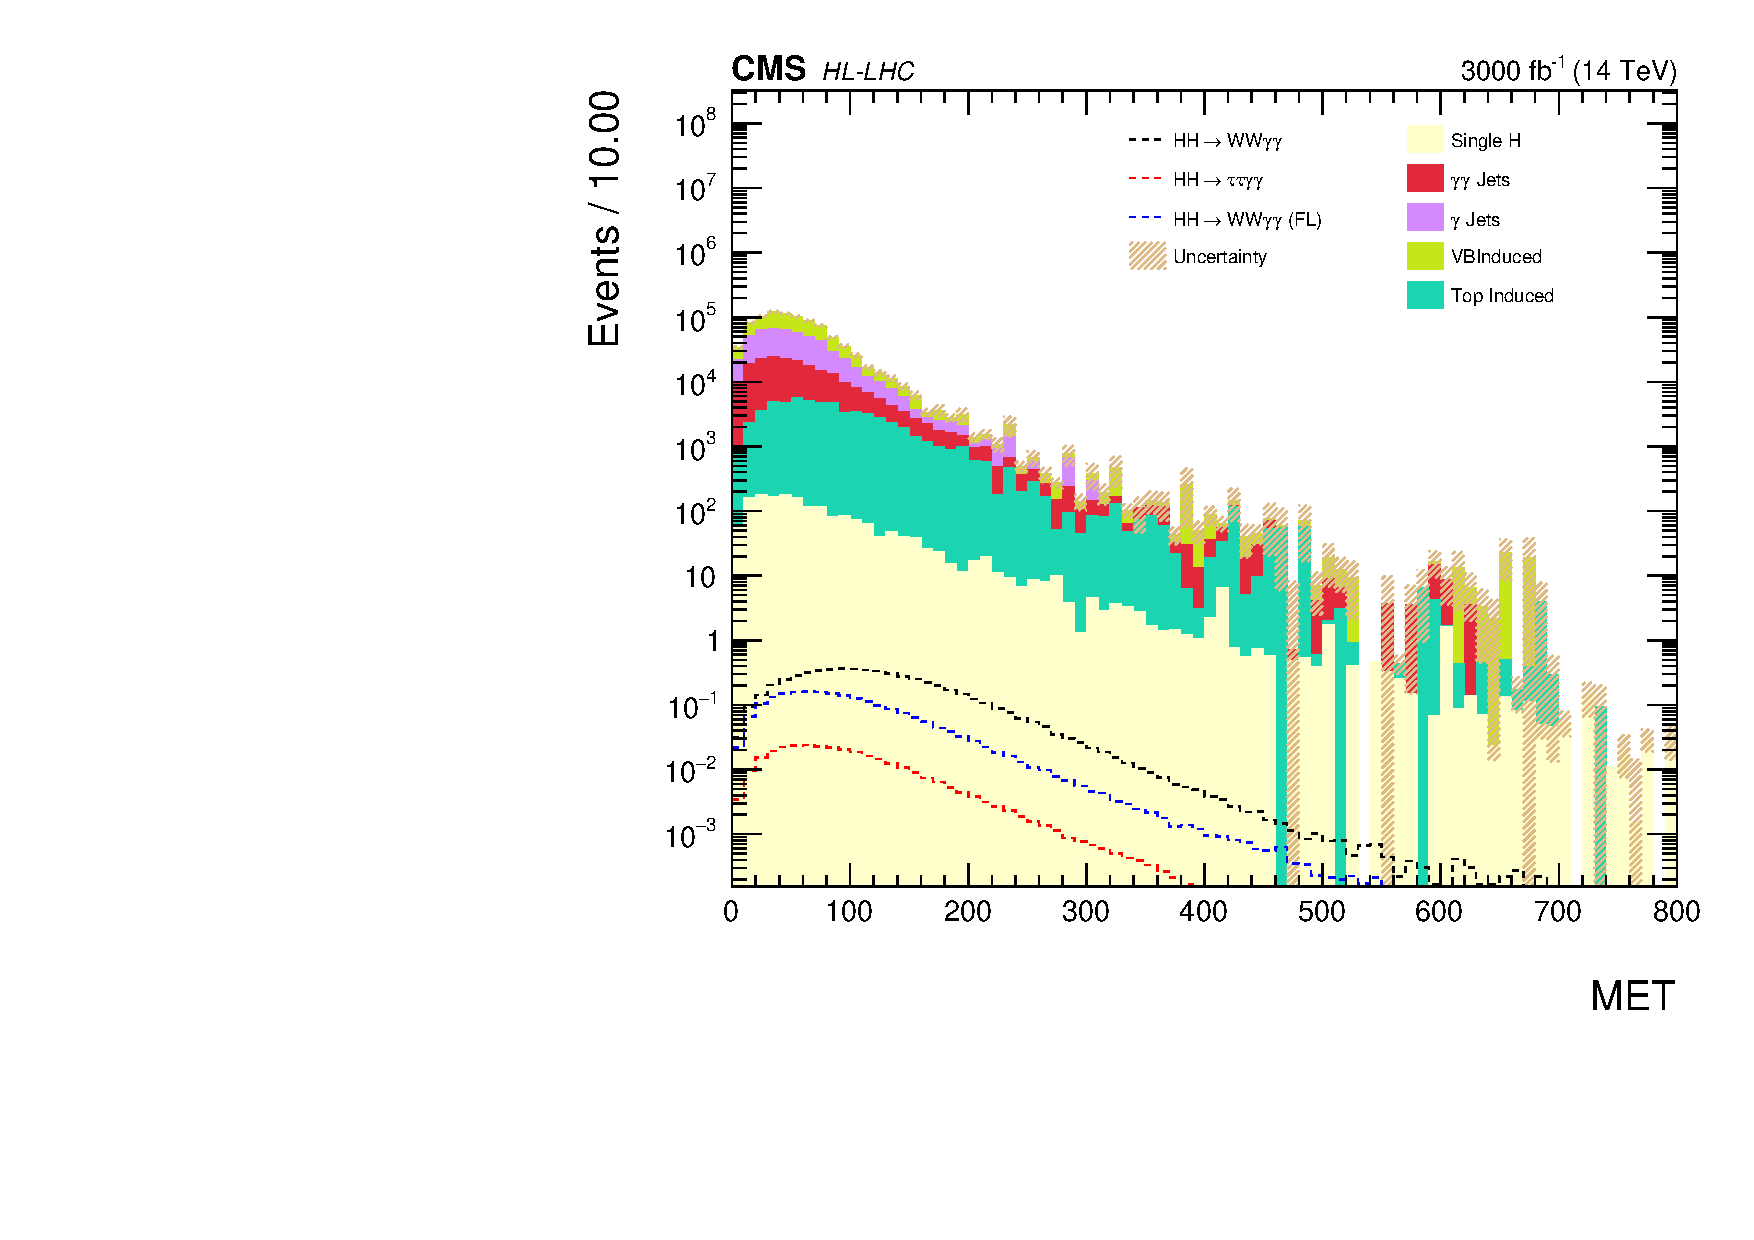
\includegraphics[width=\textwidth]{MET_logy.pdf}
        \vspace{-0.5cm}
        \firstsubcaption{$E_T^{miss}$}   
    \end{subfigure}
    \caption{\small DNN input distributions for the semi-leptonic channel of $HH\rightarrow{WW\gamma\gamma}$ (continued).}
\end{figure*}

\begin{figure*}[h!]
    \centering
    \begin{subfigure}[b]{0.475\textwidth}
        \centering
        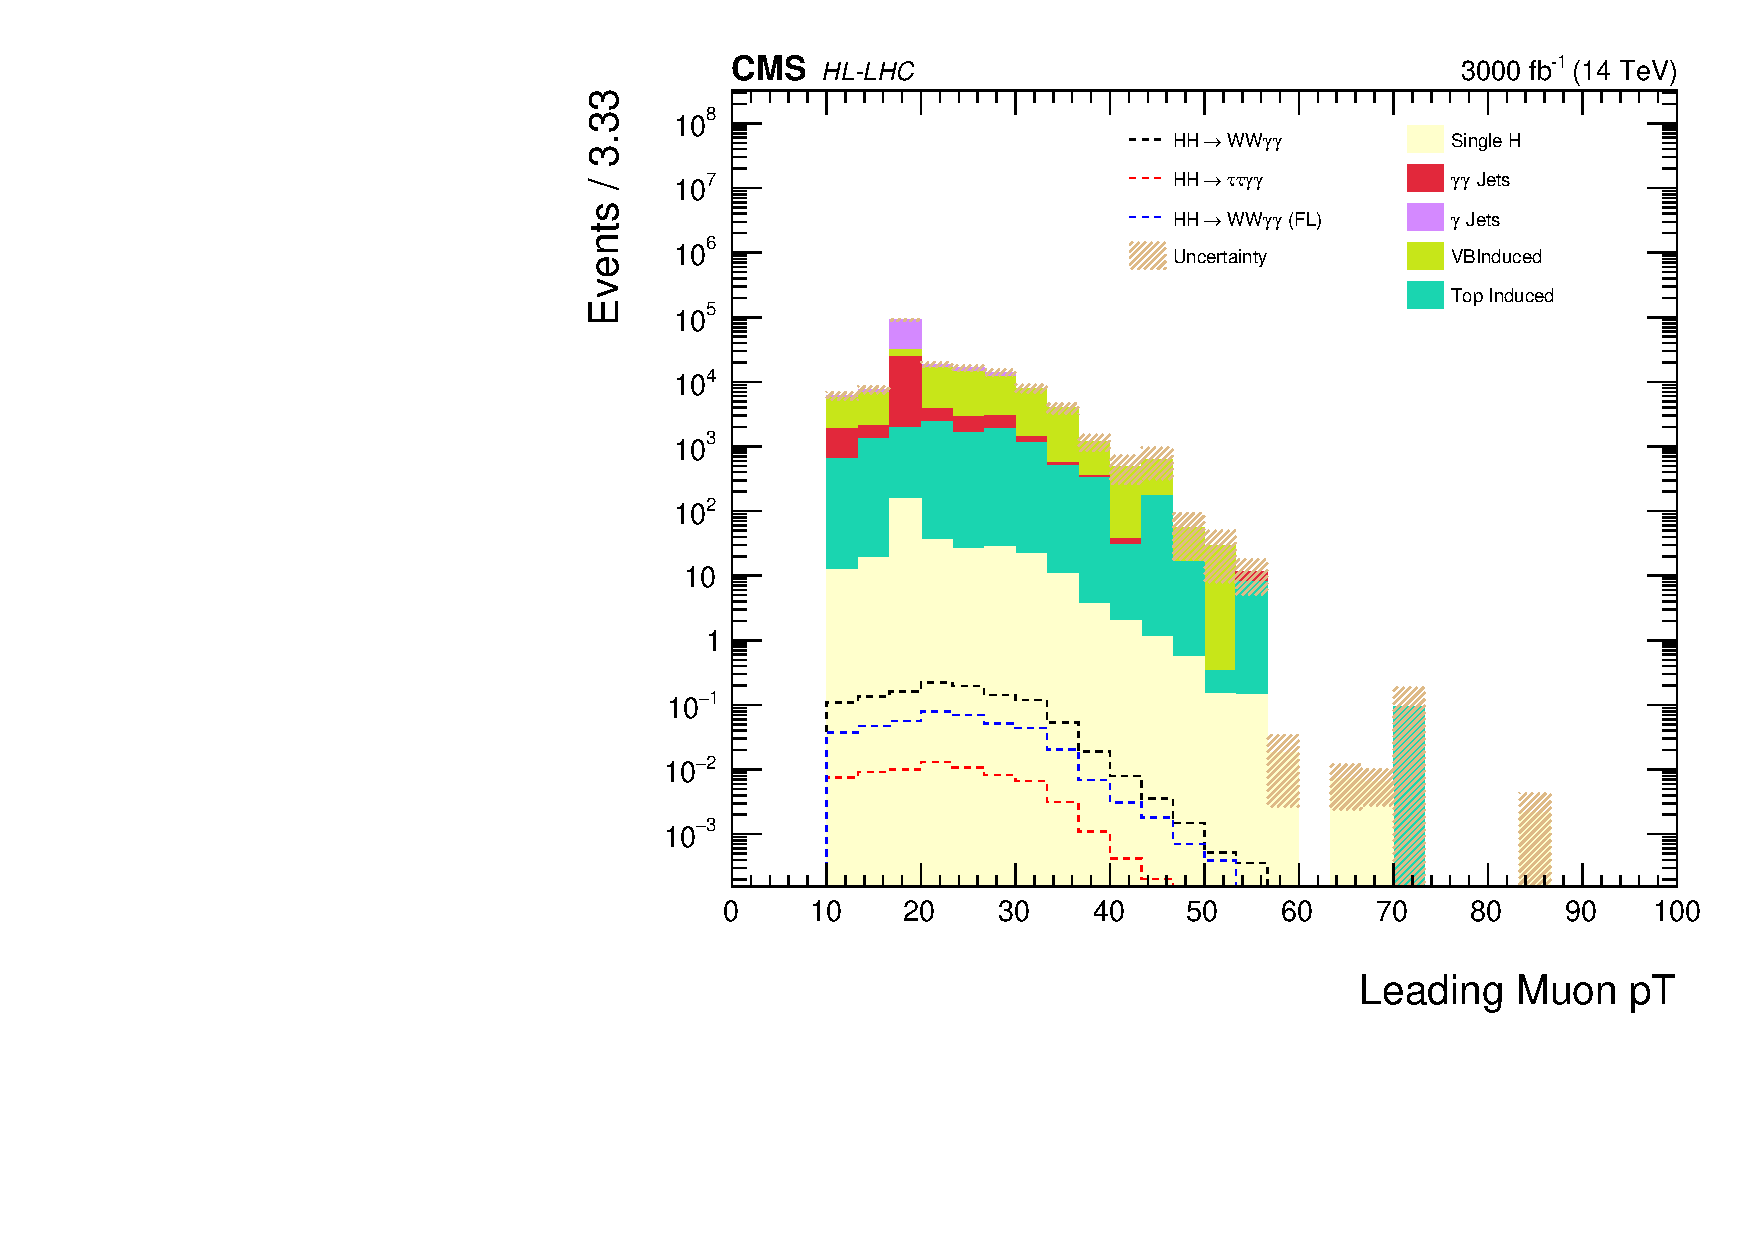
\includegraphics[width=\textwidth]{MuonpT_logy.pdf}
        \vspace{-0.5cm}
        \firstsubcaption{Sub-leading Photon $\phi$}
    \end{subfigure}
    \hfill
    \begin{subfigure}[b]{0.475\textwidth}  
        \centering 
        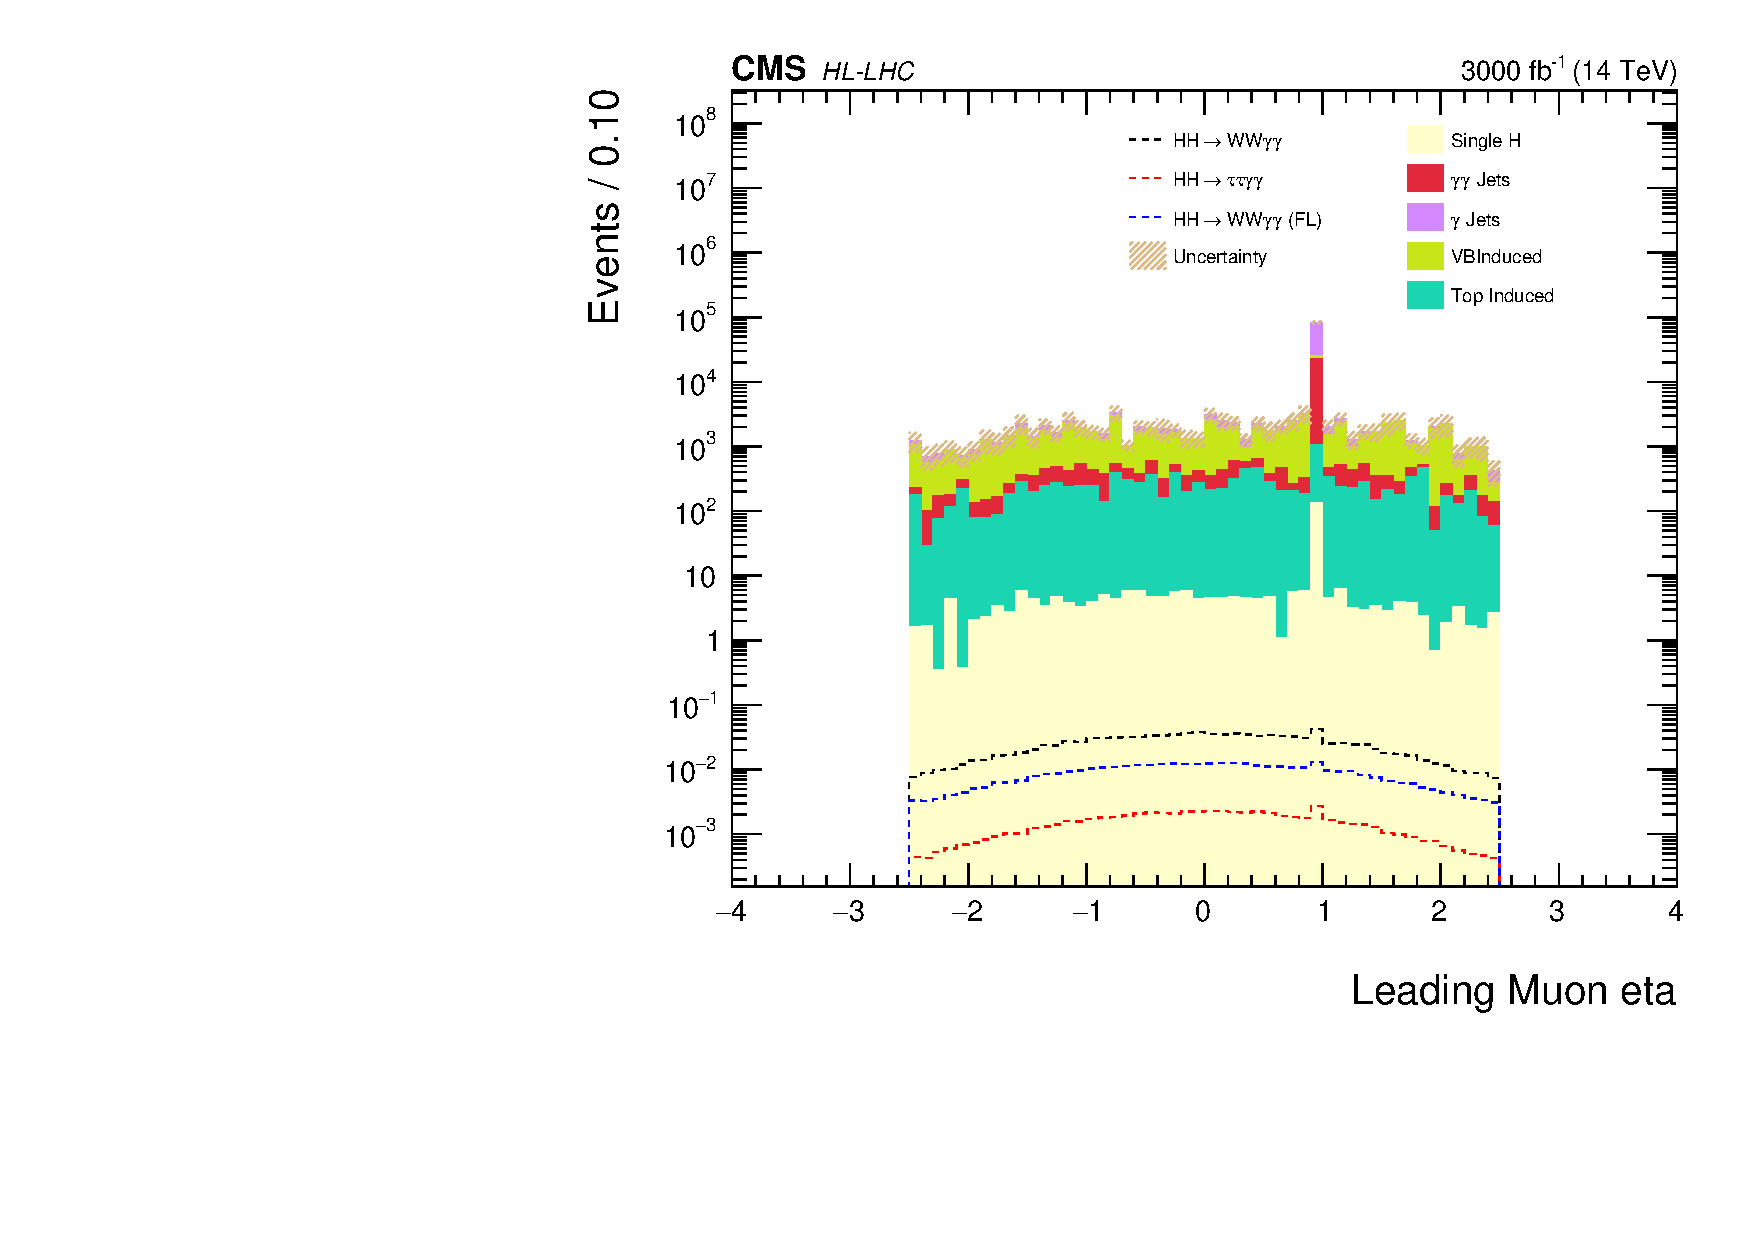
\includegraphics[width=\textwidth]{MuonEta_logy.pdf}
        \vspace{-0.5cm}
        \firstsubcaption{Jet Multiplicity}
    \end{subfigure}
    \vskip\baselineskip
    \begin{subfigure}[b]{0.475\textwidth}   
        \centering 
        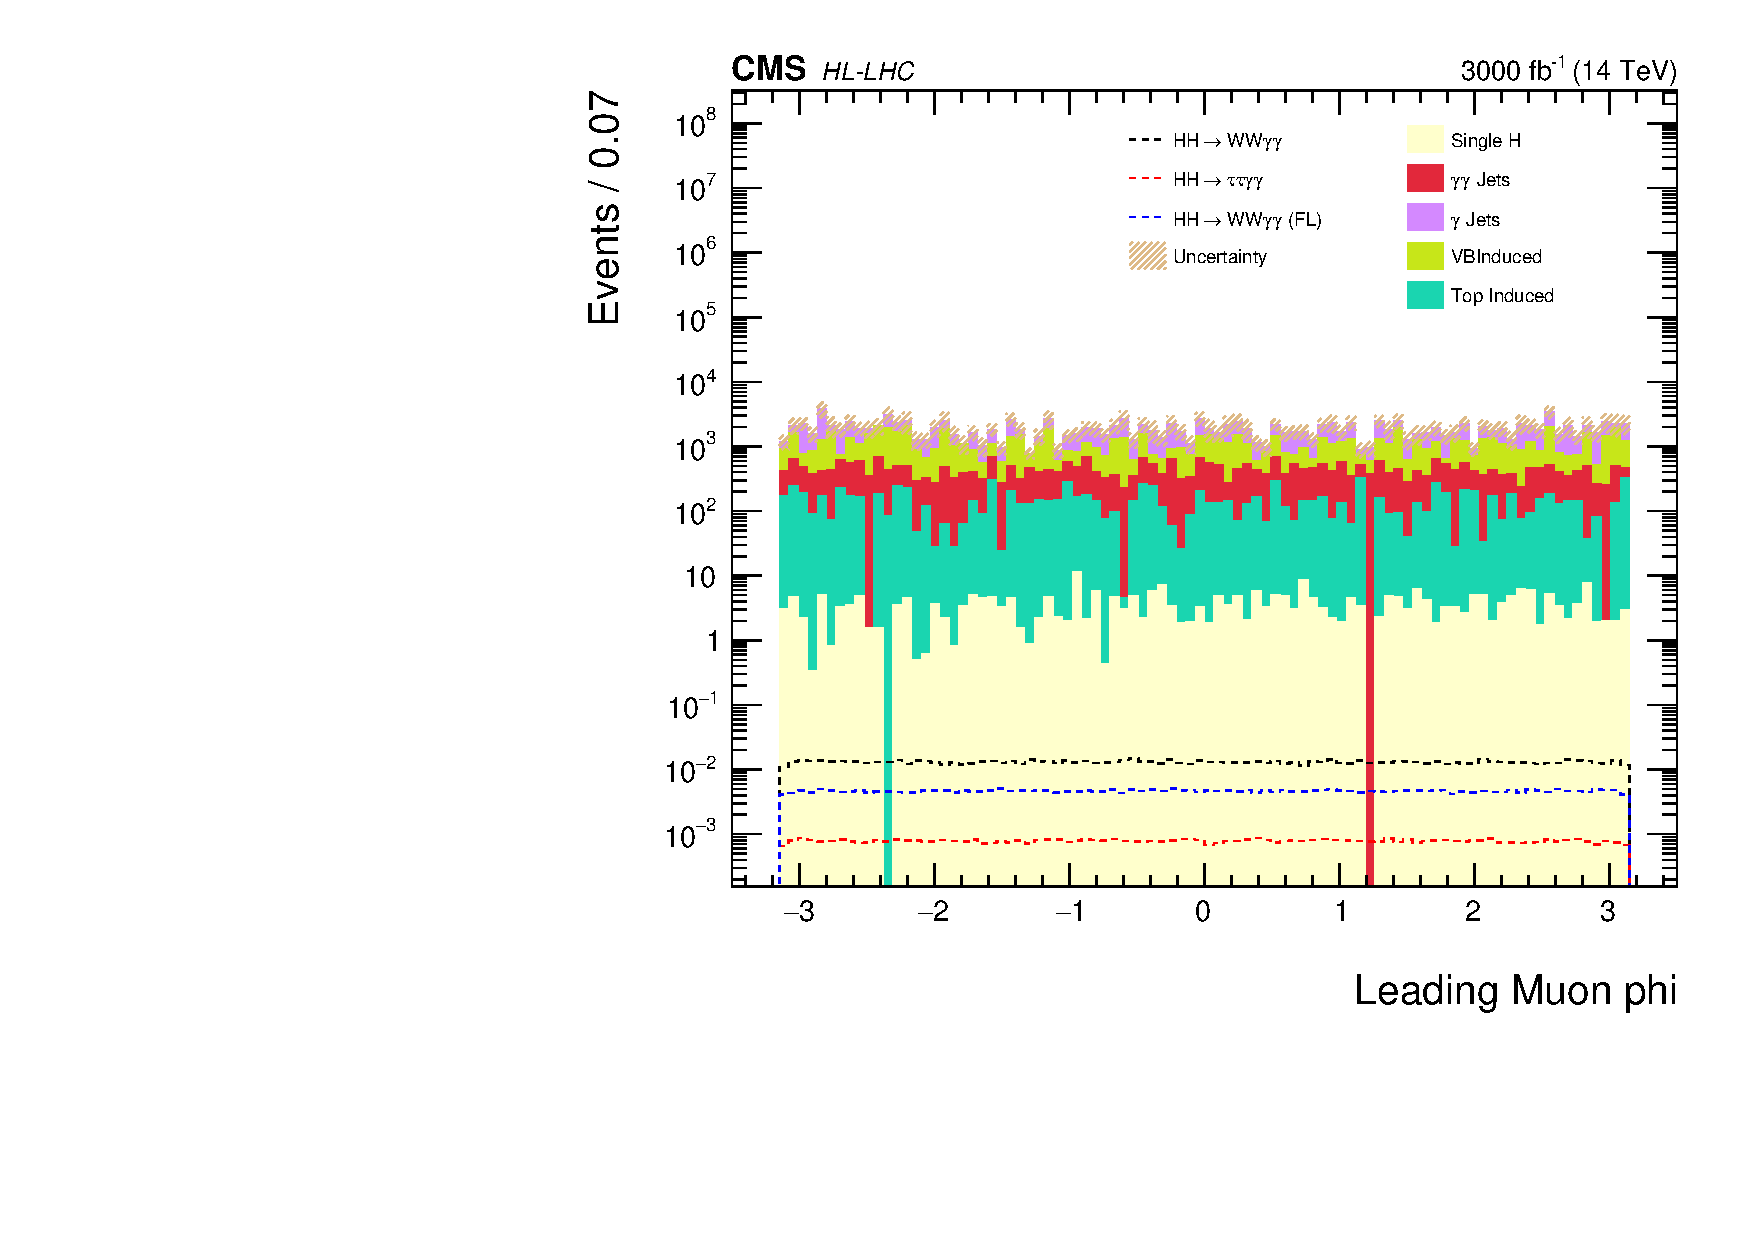
\includegraphics[width=\textwidth]{MuonPhi_logy.pdf}
        \vspace{-0.5cm}
        \firstsubcaption{Electron p$_{T}$}
    \end{subfigure}
    \hfill
    \begin{subfigure}[b]{0.475\textwidth}   
        \centering 
        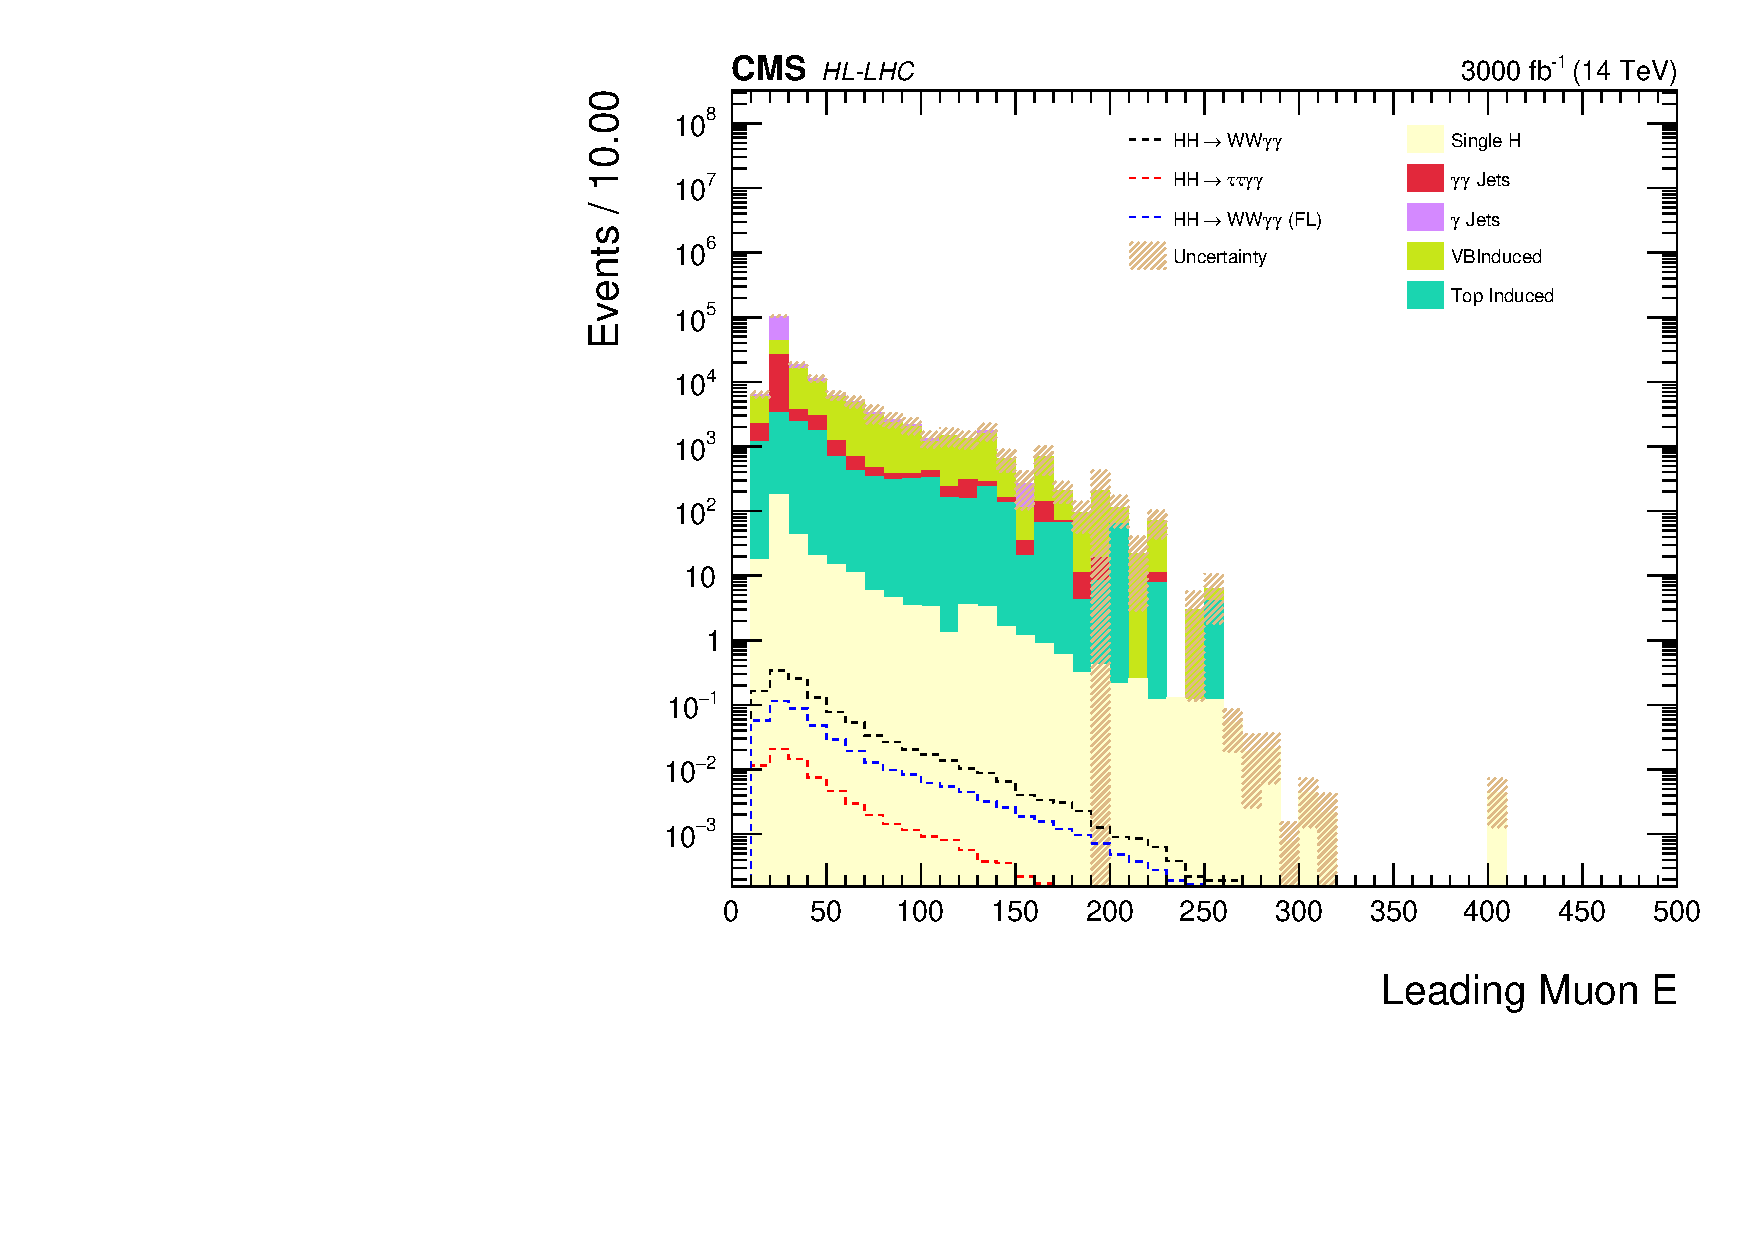
\includegraphics[width=\textwidth]{MuonE_logy.pdf}
        \vspace{-0.5cm}
        \firstsubcaption{Electron $\eta$}
    \end{subfigure}
    \vskip\baselineskip
    \begin{subfigure}[b]{0.475\textwidth}   
        \centering 
        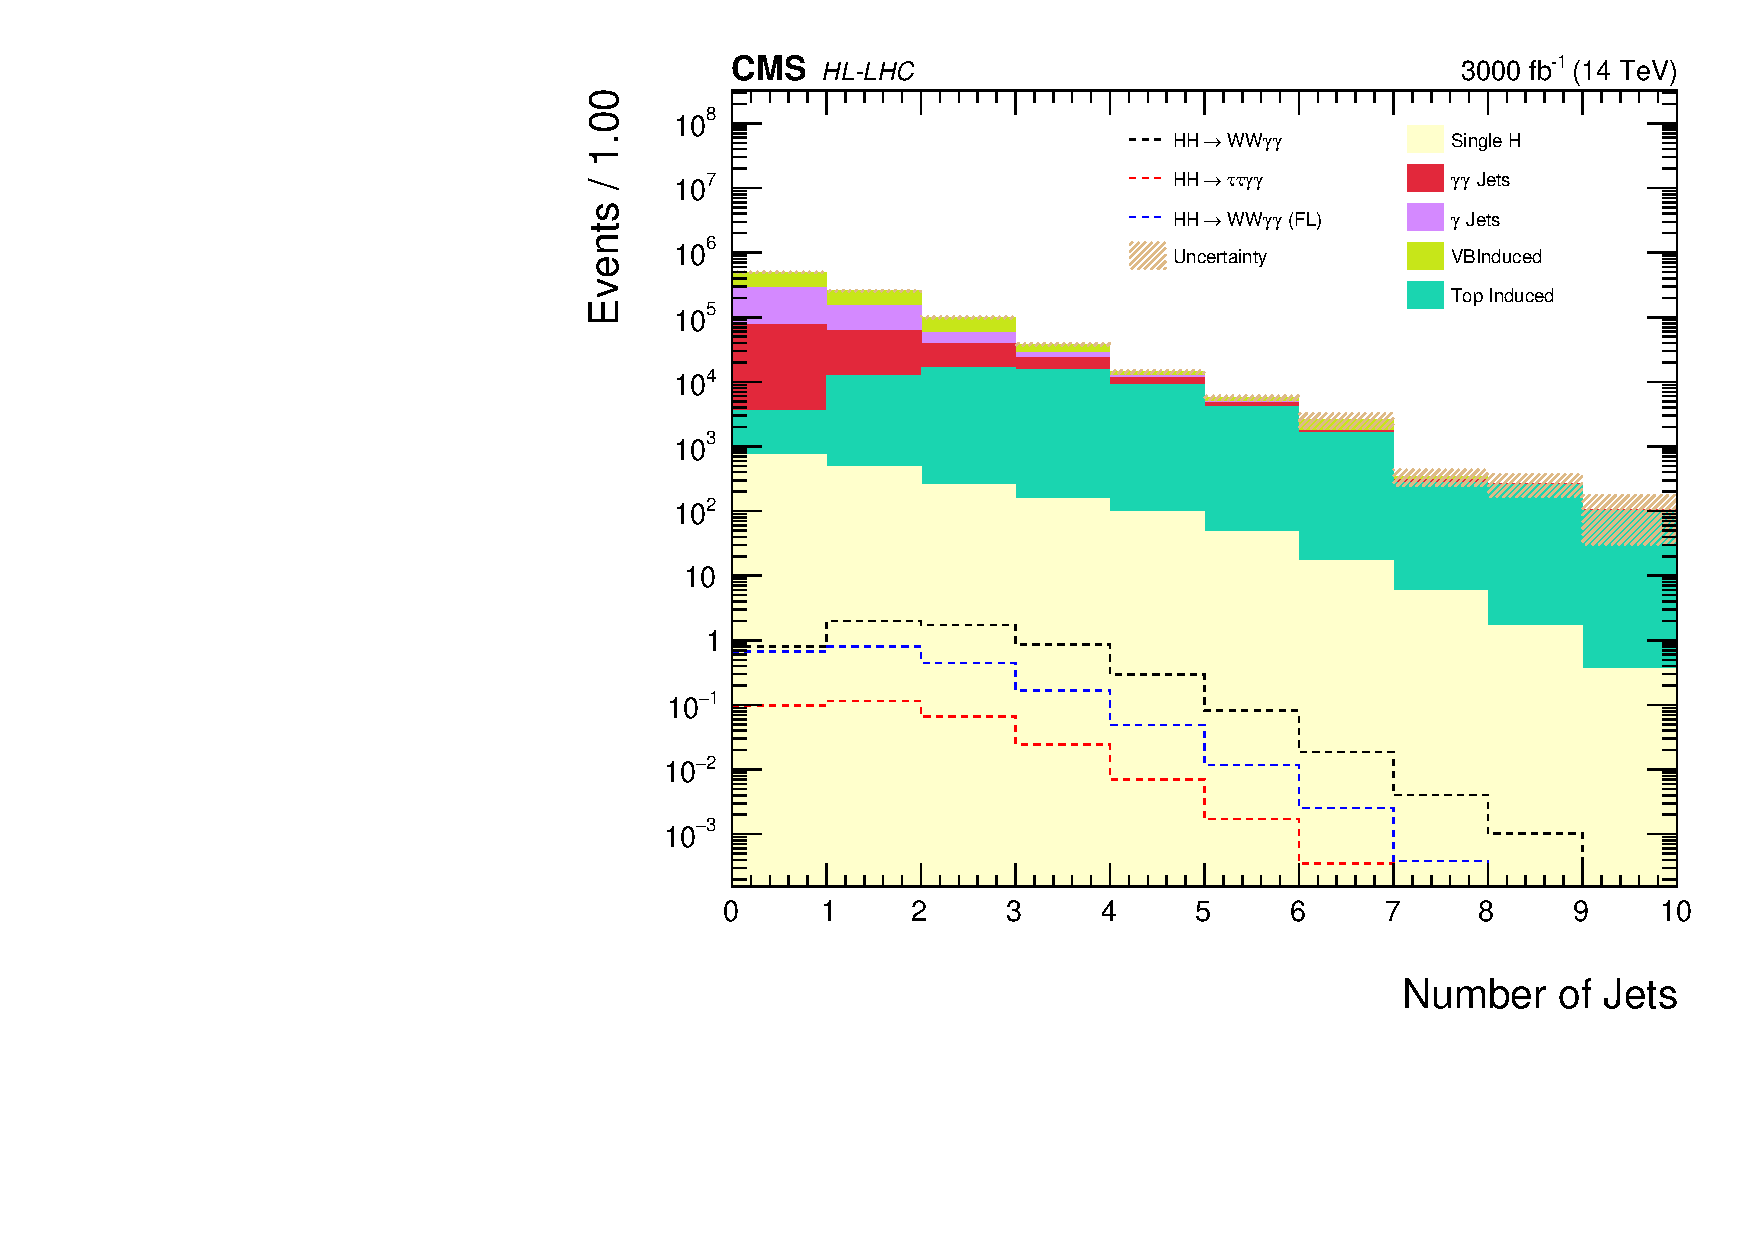
\includegraphics[width=\textwidth]{nJetsOneL_logy.pdf}
        \vspace{-0.5cm}
        \firstsubcaption{Jet multiplicity}
    \end{subfigure}
    \hfill
    \begin{subfigure}[b]{0.475\textwidth}   
        \centering 
        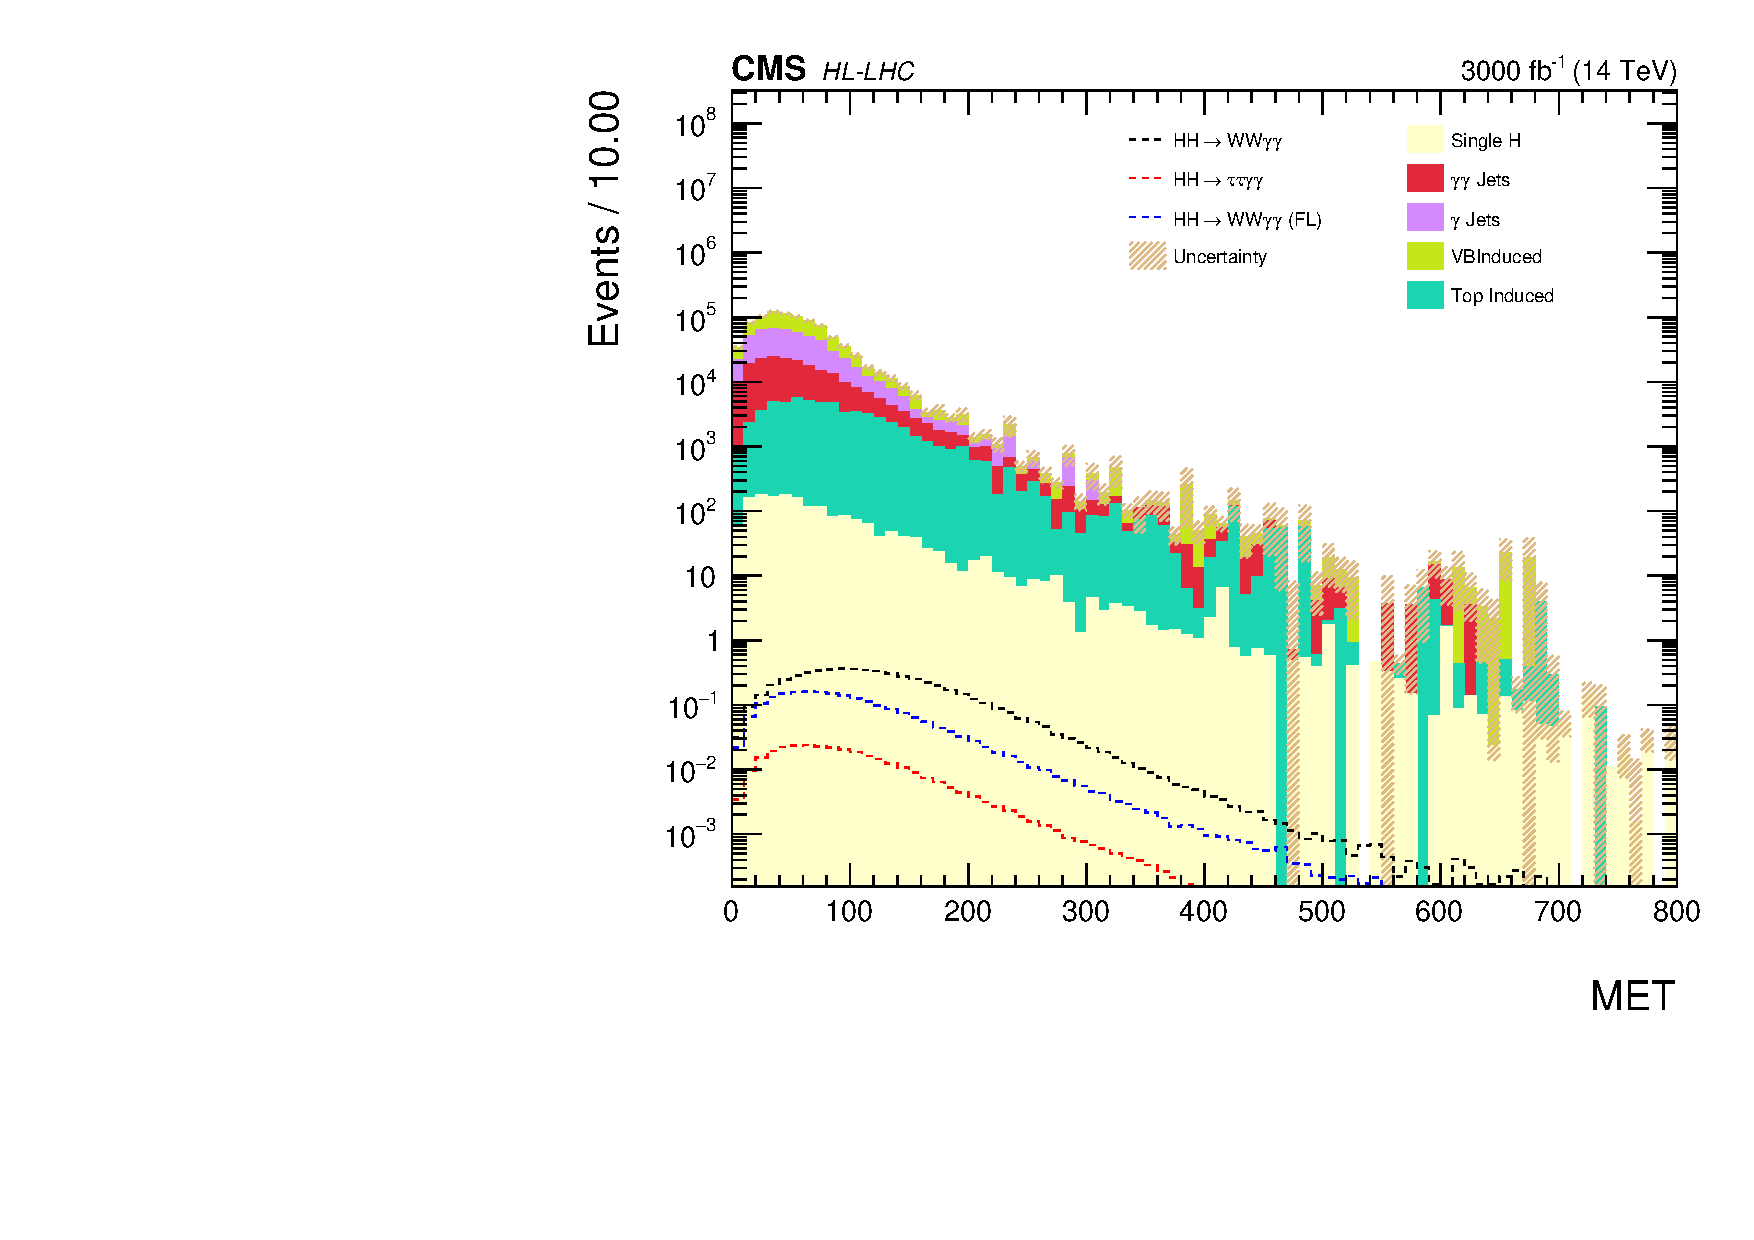
\includegraphics[width=\textwidth]{MET_logy.pdf}
        \vspace{-0.5cm}
        \firstsubcaption{$E_T^{miss}$}   
    \end{subfigure}
    \caption{\small DNN input distributions for the semi-leptonic channel of $HH\rightarrow{WW\gamma\gamma}$ (continued).}
\end{figure*}

\begin{figure*}[h!]
    \centering
    \begin{subfigure}[b]{0.475\textwidth}
        \centering
        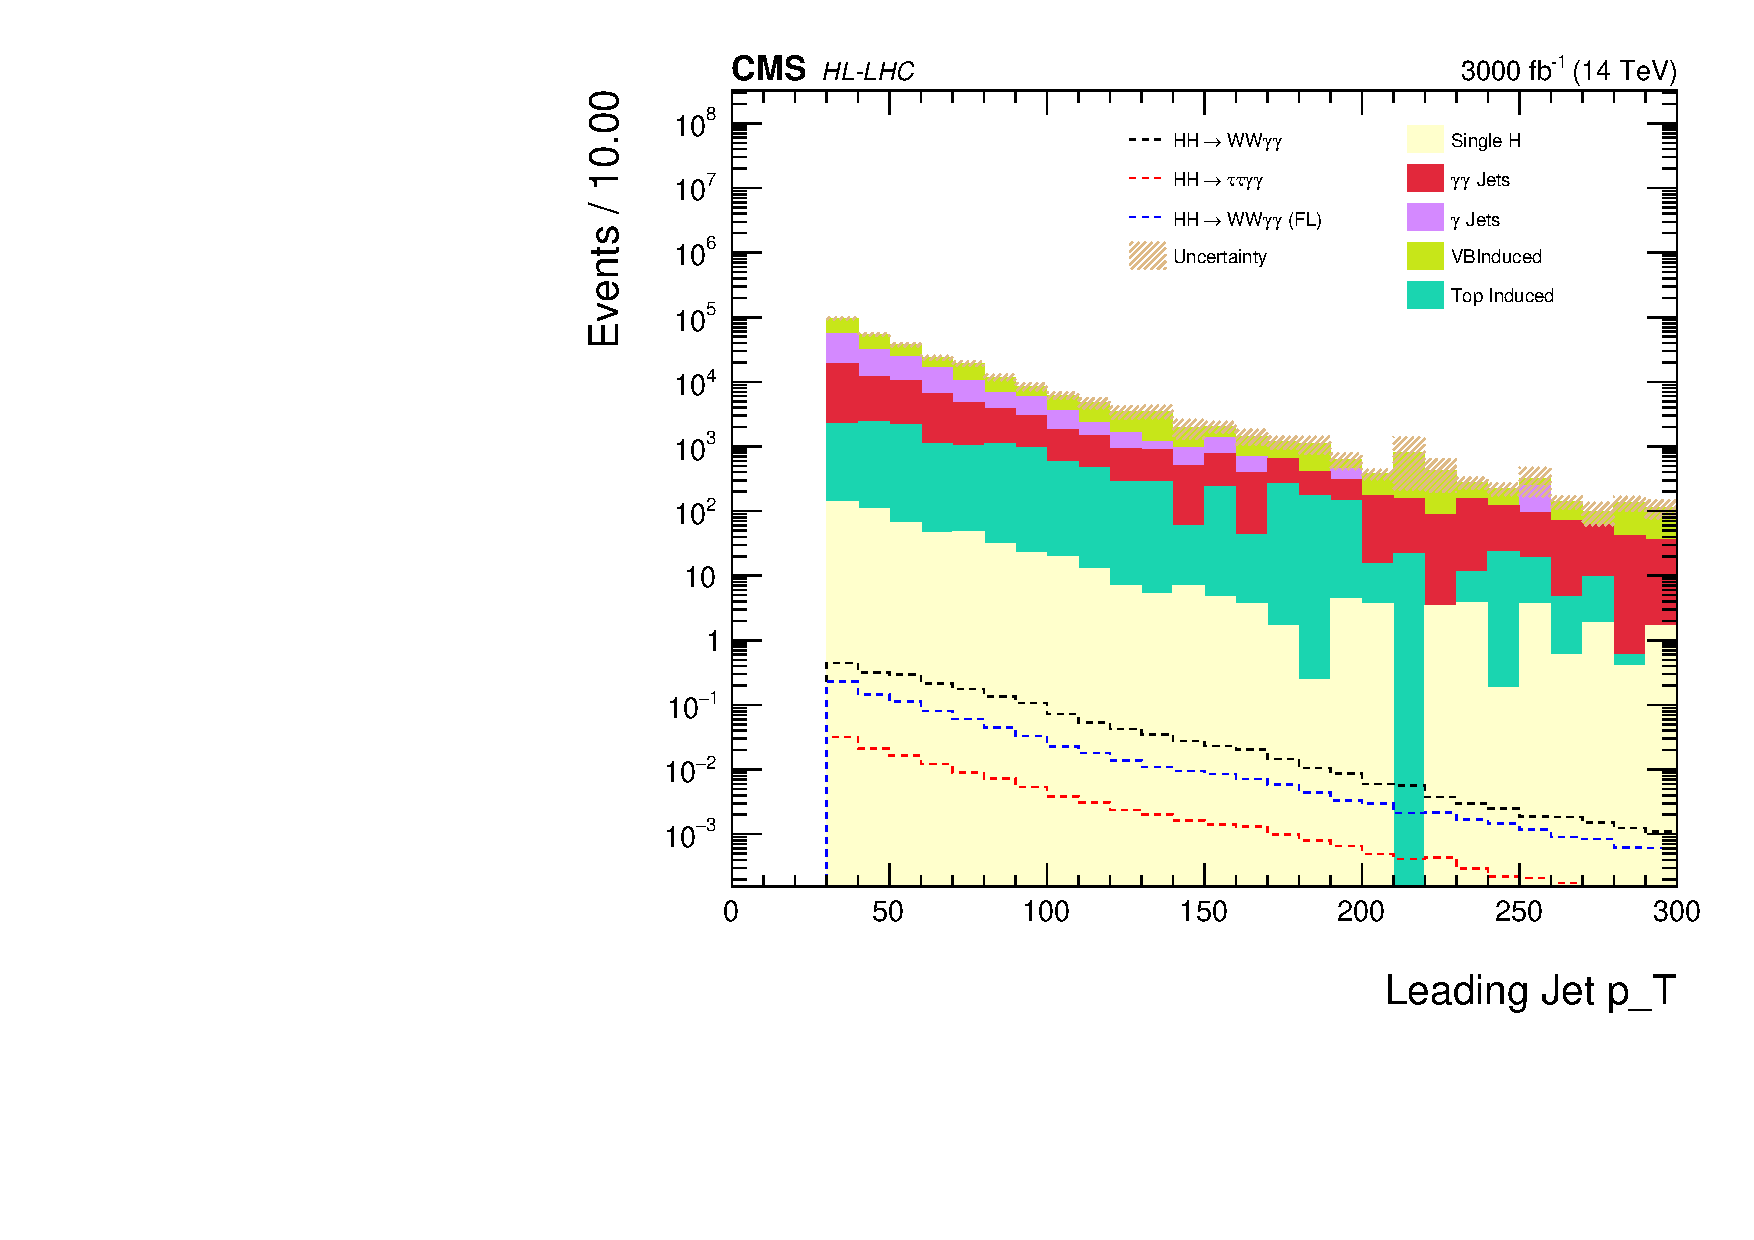
\includegraphics[width=\textwidth]{hasonel_hasOneJ_jetpt_logy.pdf}
        \vspace{-0.5cm}
        \firstsubcaption{Leading jet \pt}
    \end{subfigure}
    \hfill
    \begin{subfigure}[b]{0.475\textwidth}  
        \centering 
        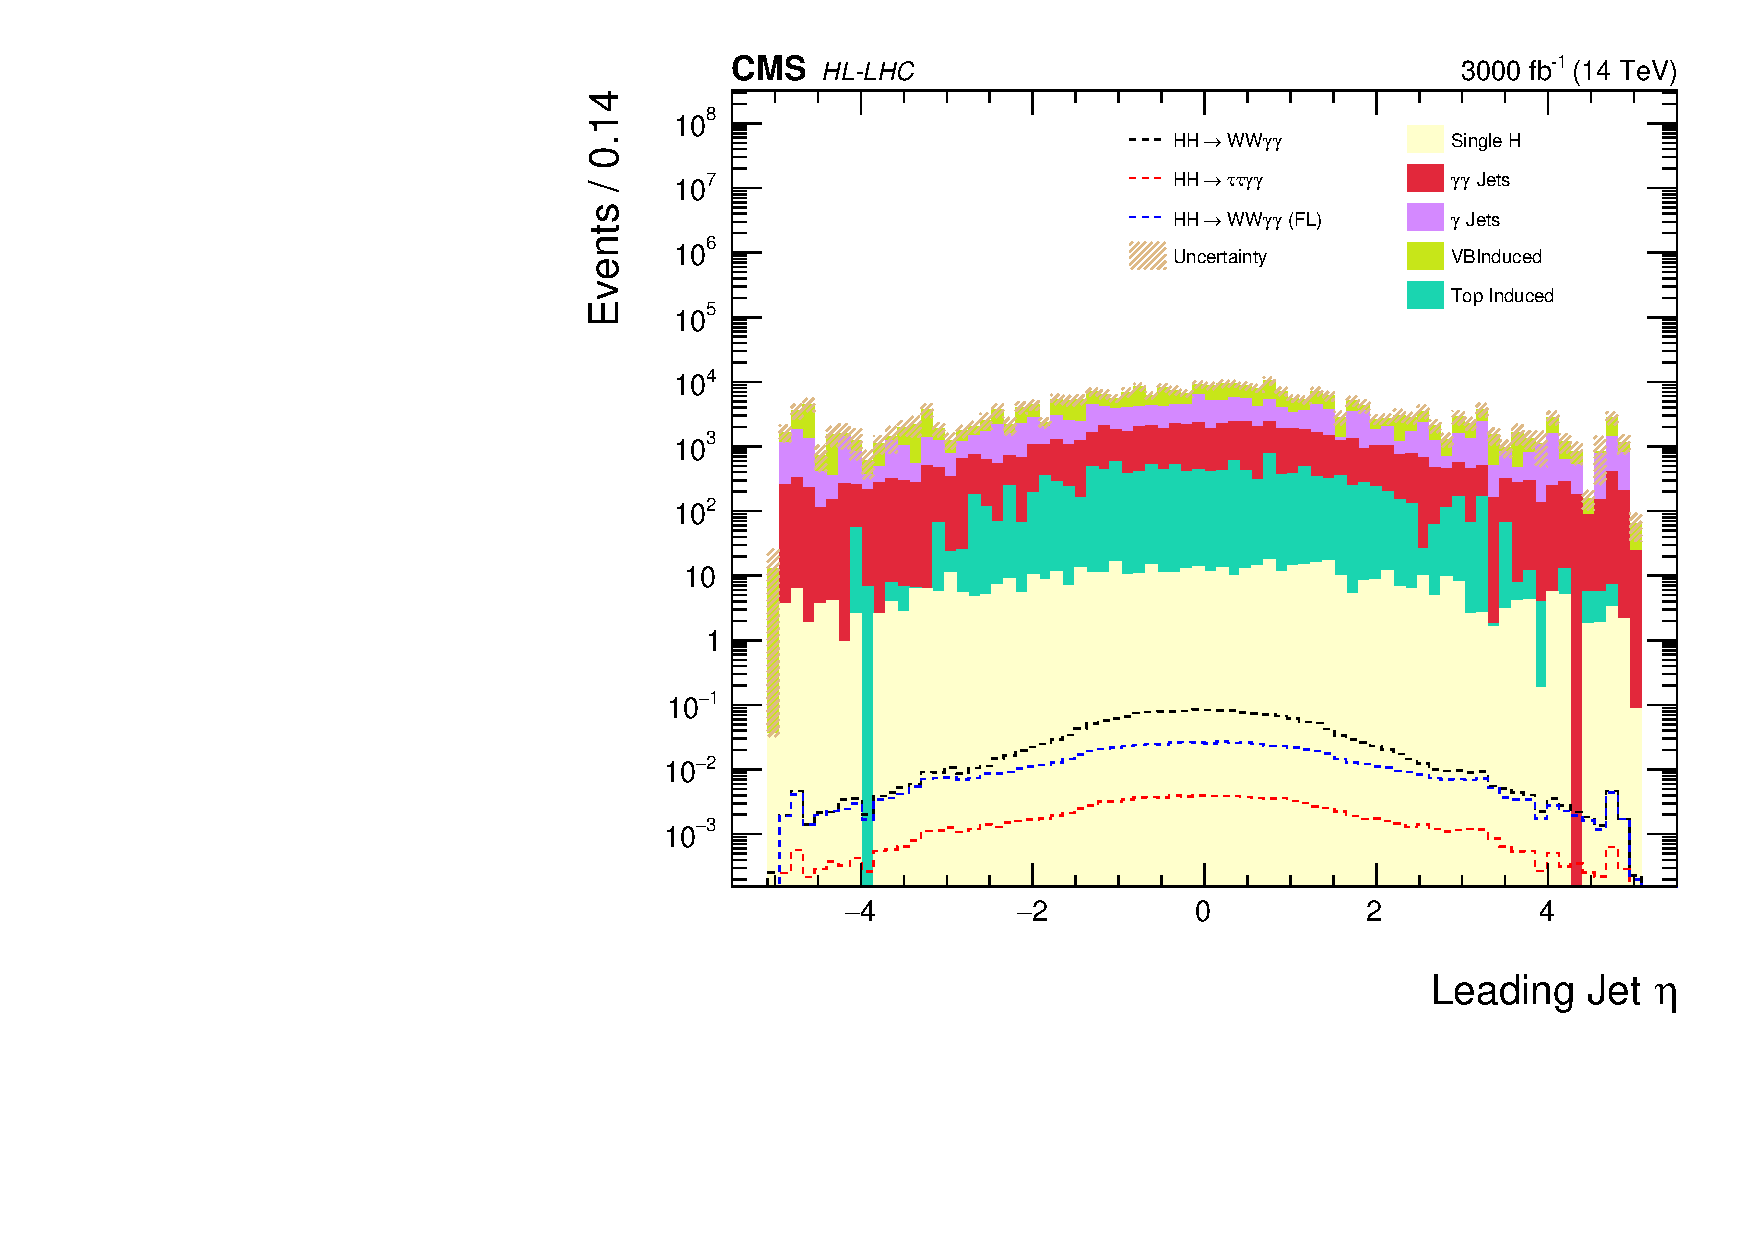
\includegraphics[width=\textwidth]{hasonel_hasOneJ_jeteta_logy.pdf}
        \vspace{-0.5cm}
        \firstsubcaption{Leading jet $\eta$}
    \end{subfigure}
    \vskip\baselineskip
    \begin{subfigure}[b]{0.475\textwidth}   
        \centering 
        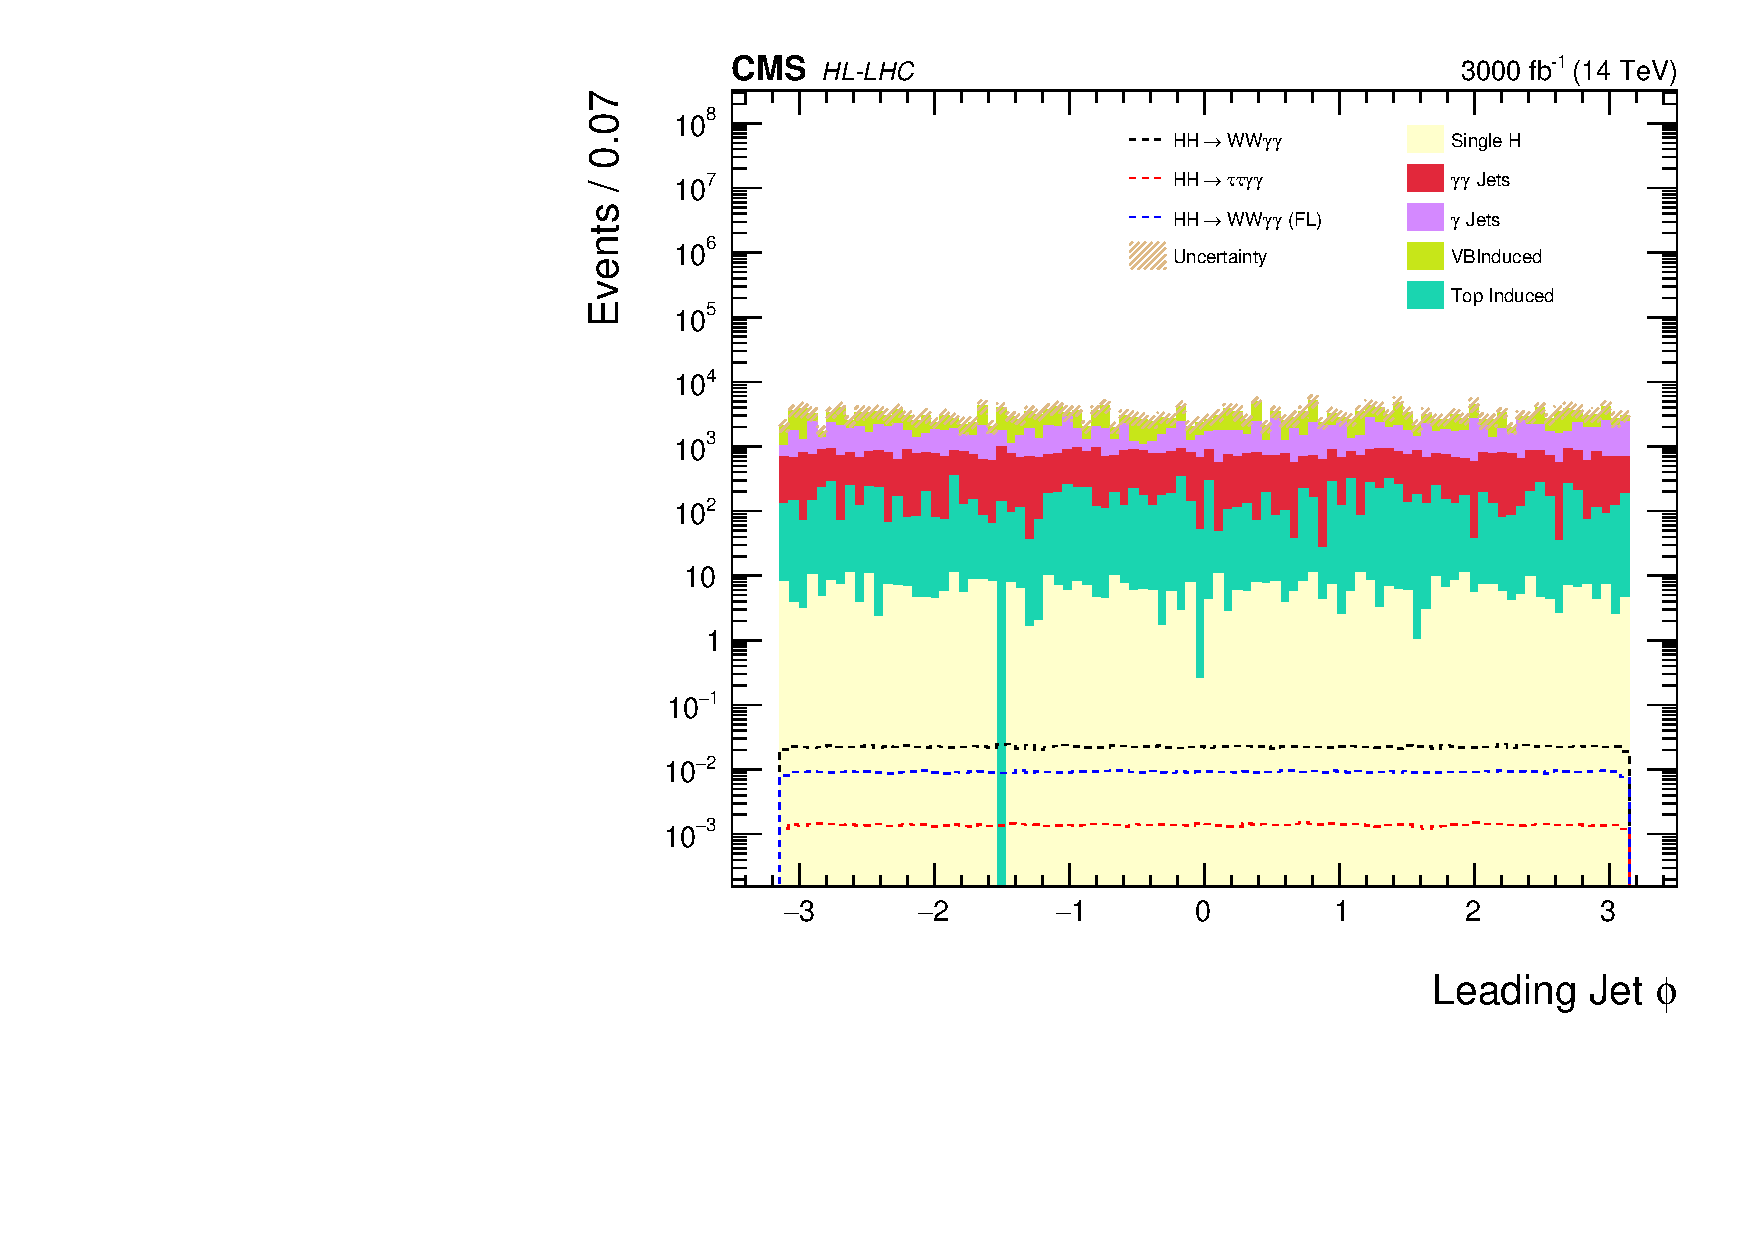
\includegraphics[width=\textwidth]{hasonel_hasOneJ_jetphi_logy.pdf}
        \vspace{-0.5cm}
        \firstsubcaption{Leading jet $\phi$}
    \end{subfigure}
    \hfill
    \begin{subfigure}[b]{0.475\textwidth}   
        \centering 
        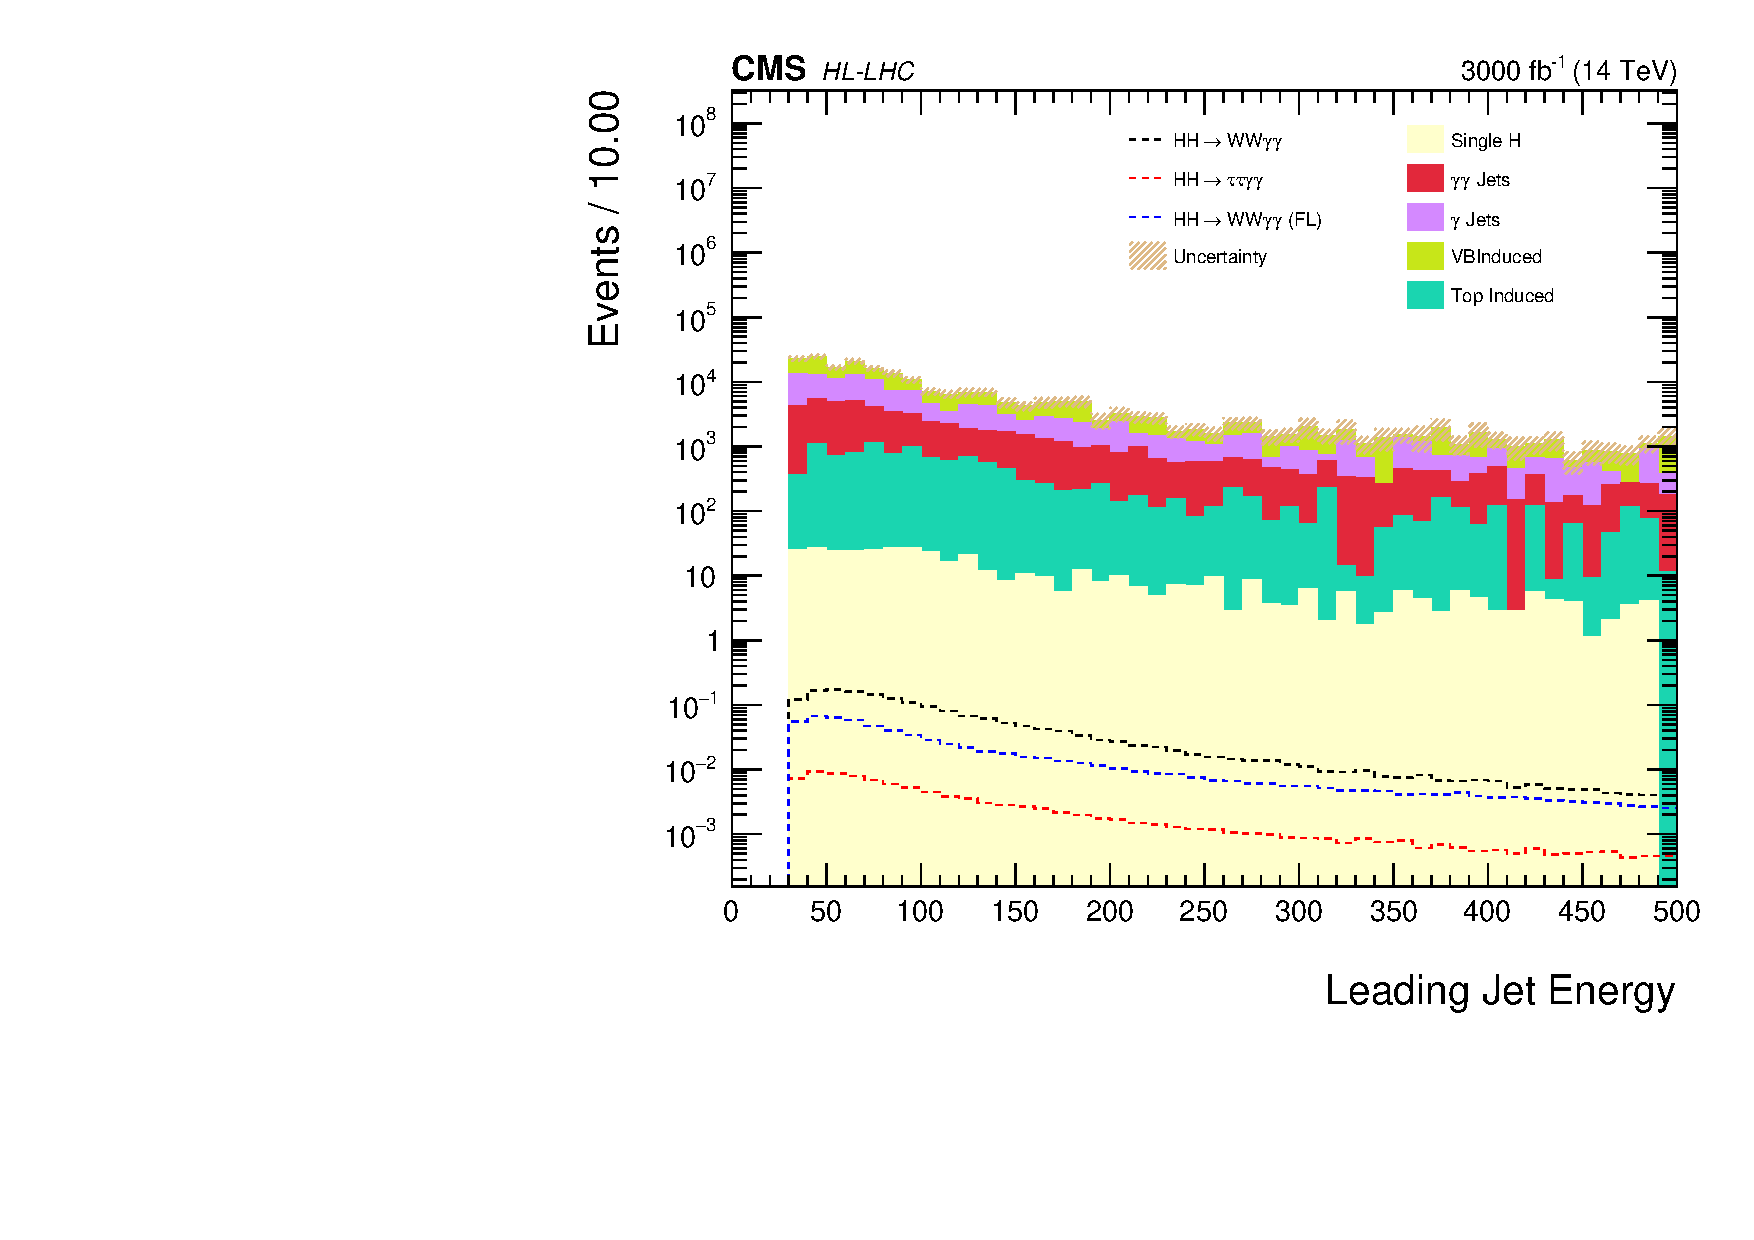
\includegraphics[width=\textwidth]{hasonel_hasOneJ_jetE_logy.pdf}
        \vspace{-0.5cm}
        \firstsubcaption{Leading jet energy}
    \end{subfigure}
    \vskip\baselineskip
    \begin{subfigure}[b]{0.475\textwidth}   
        \centering 
        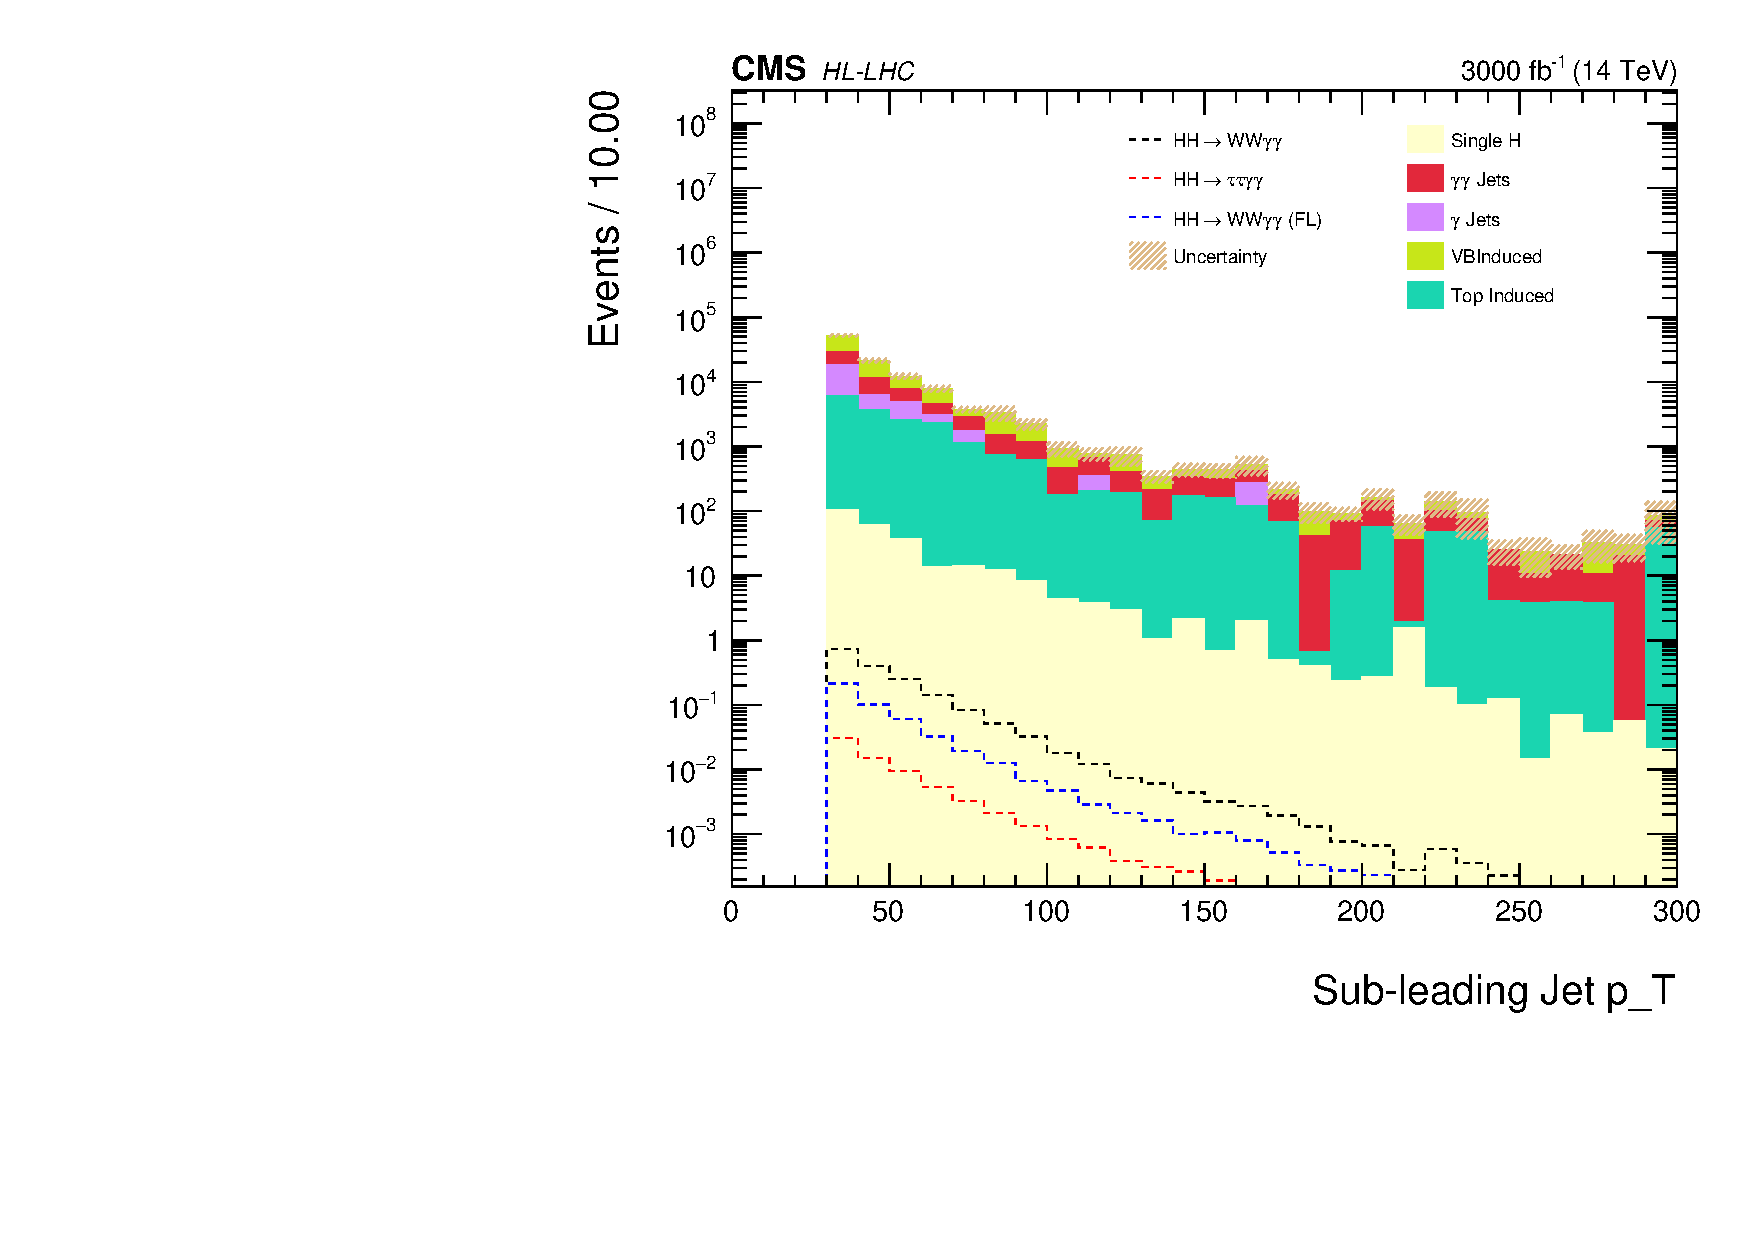
\includegraphics[width=\textwidth]{hasonel_hasTwoJ_jetpt_logy.pdf}
        \vspace{-0.5cm}
        \firstsubcaption{Sub-leading jet \pt}
    \end{subfigure}
    \hfill
    \begin{subfigure}[b]{0.475\textwidth}   
        \centering 
        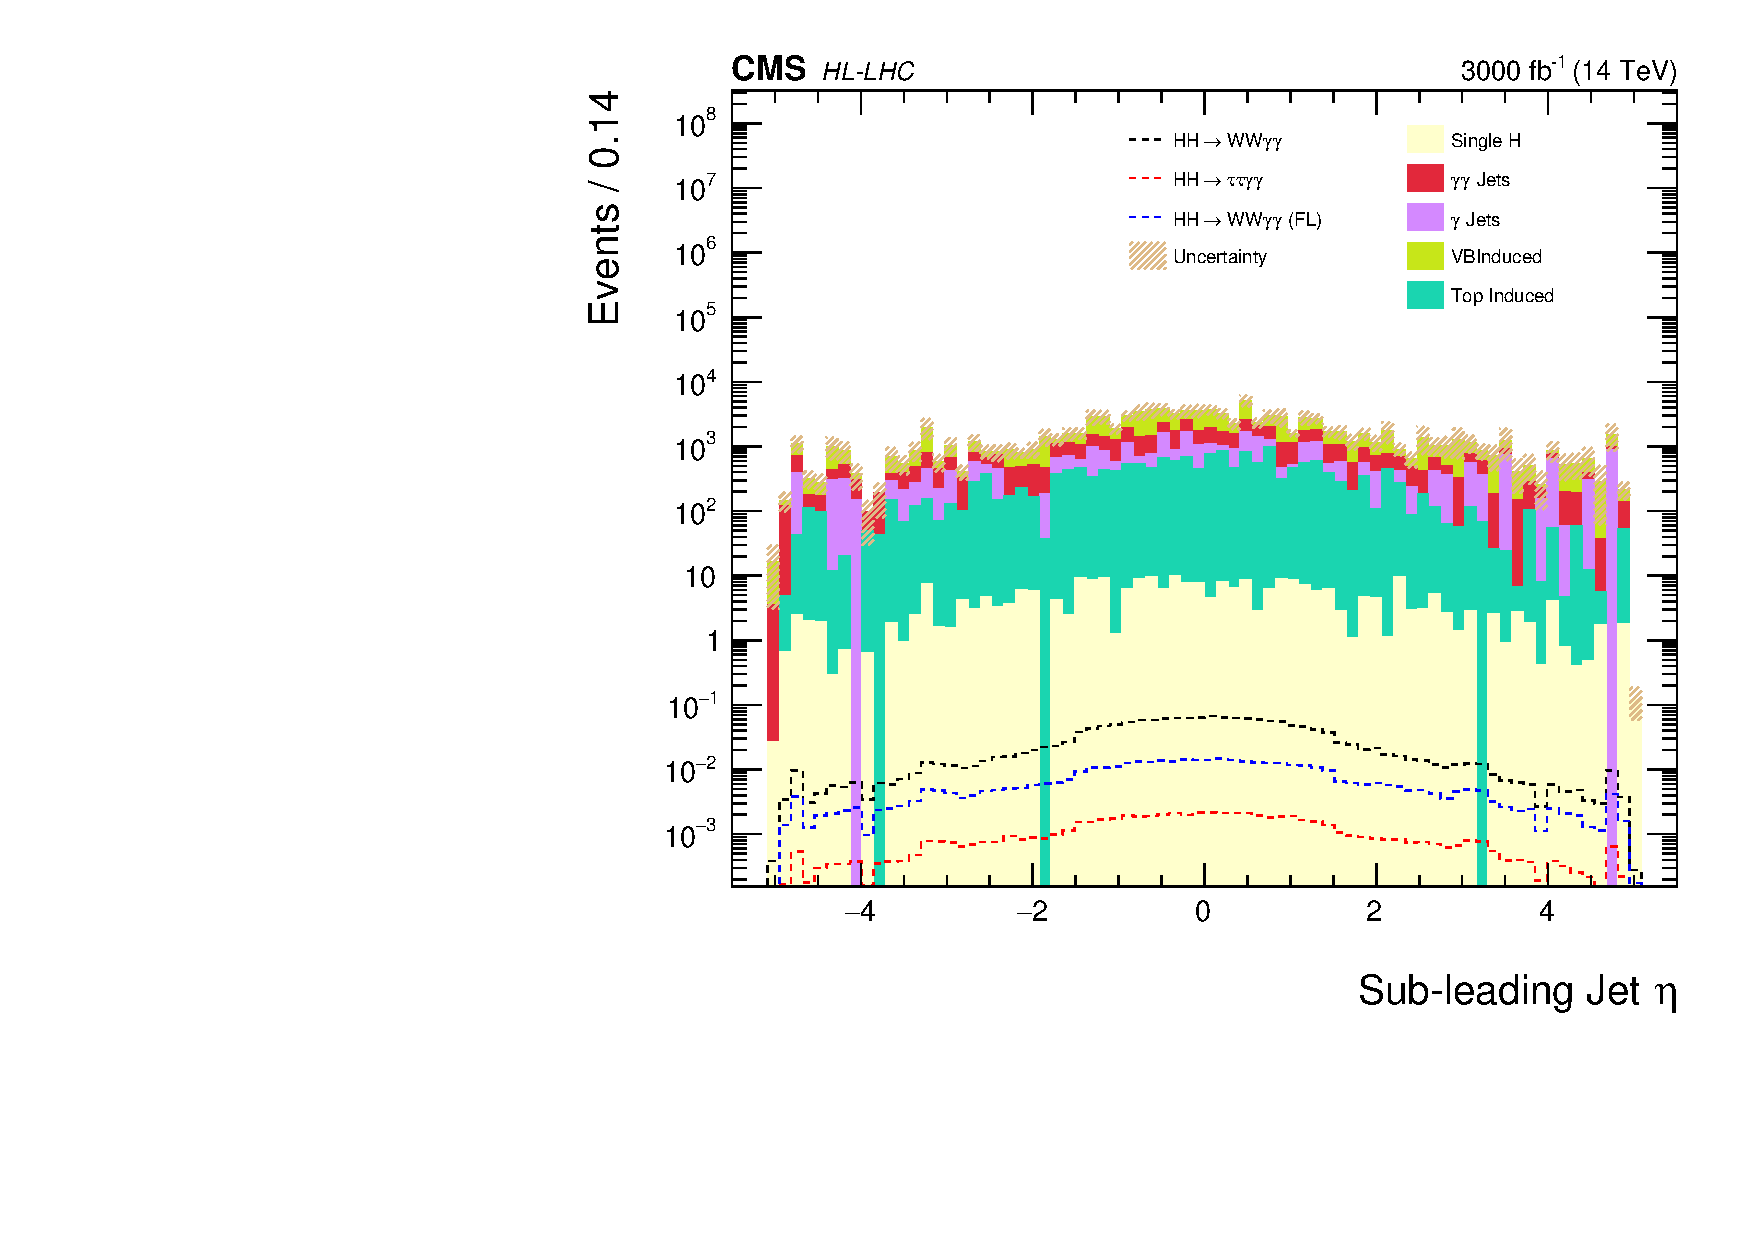
\includegraphics[width=\textwidth]{hasonel_hasTwoJ_jeteta_logy.pdf}
        \vspace{-0.5cm}
        \firstsubcaption{Sub-leading jet $\eta$}   
    \end{subfigure}
    \caption{\small DNN input distributions for the semi-leptonic channel of $HH\rightarrow{WW\gamma\gamma}$ (continued).}
\end{figure*}

\begin{figure*}[h!]
    \centering
    \begin{subfigure}[b]{0.475\textwidth}
        \centering
        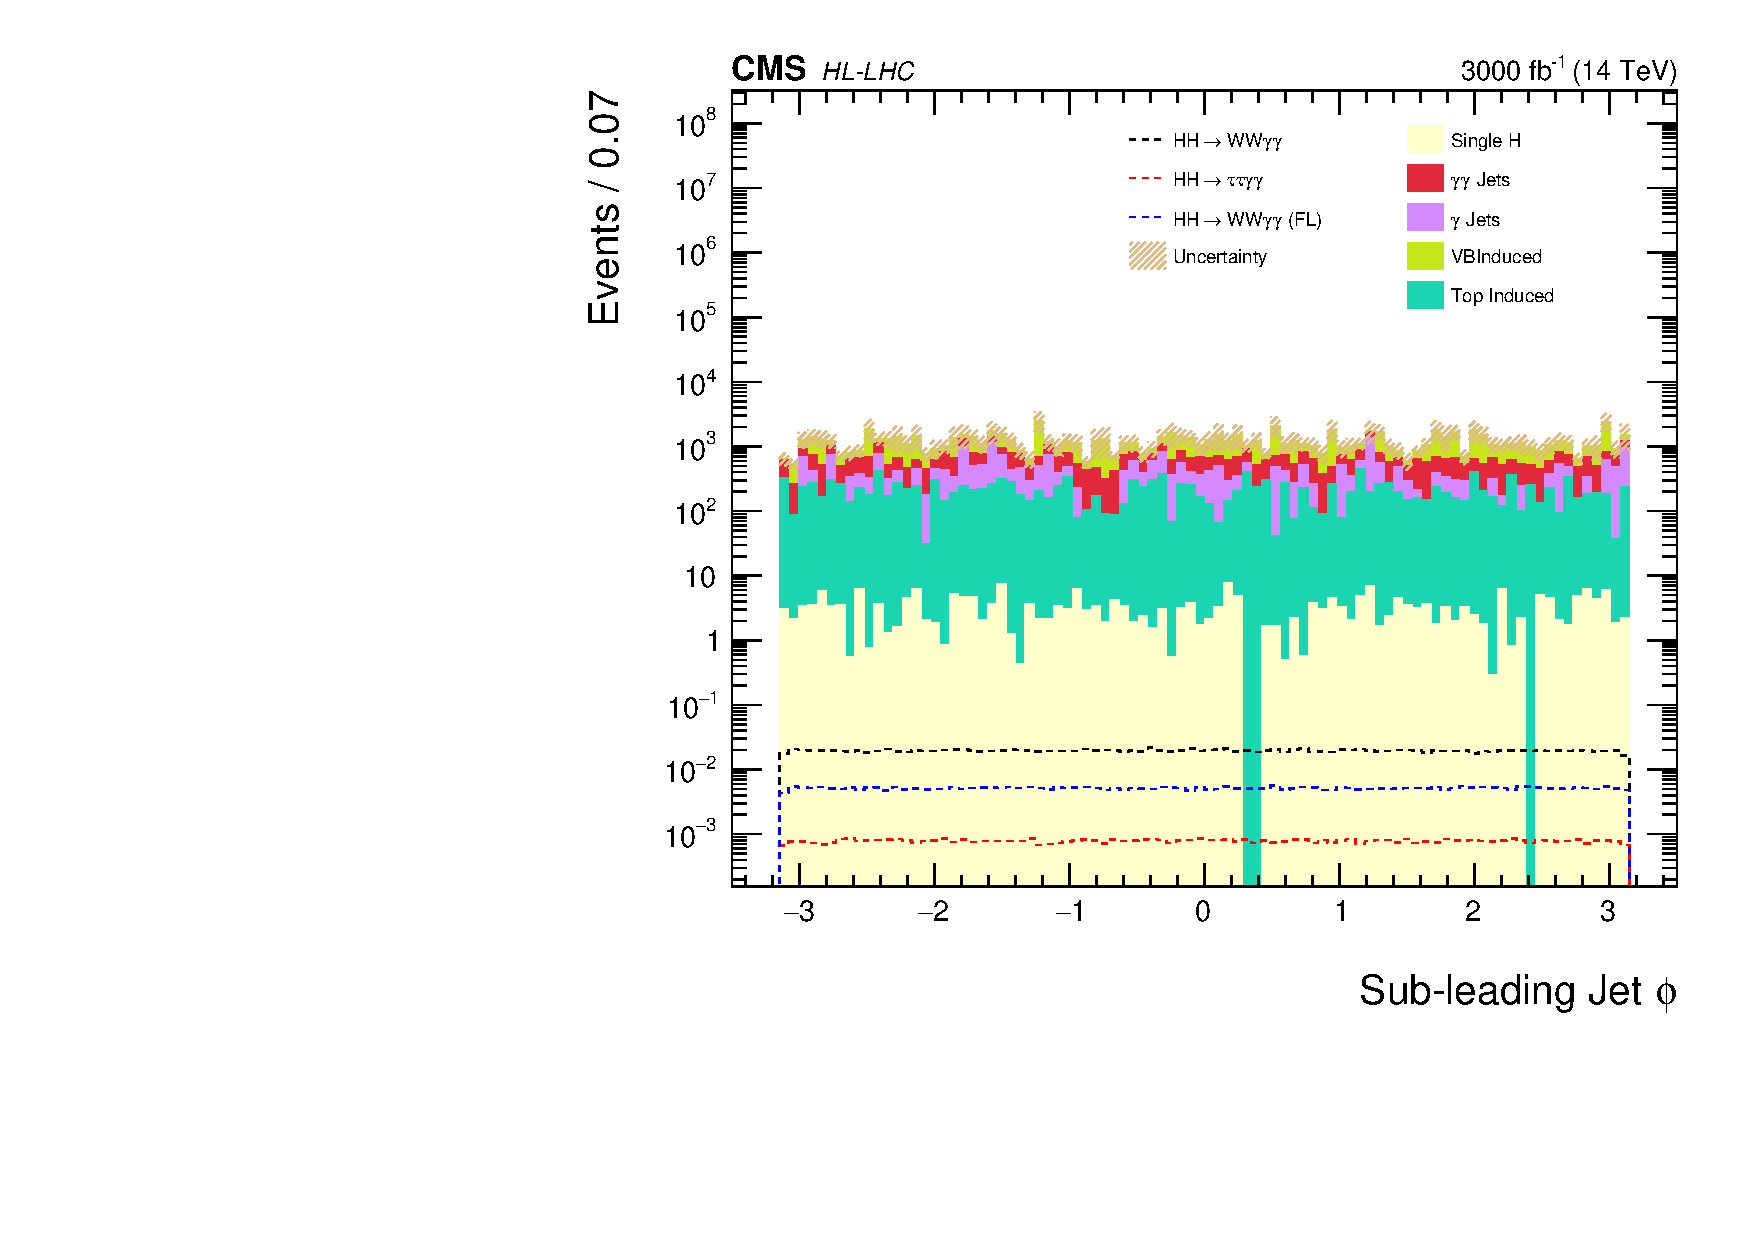
\includegraphics[width=\textwidth]{hasonel_hasTwoJ_jetphi_logy.pdf}
        \vspace{-0.5cm}
        \firstsubcaption{Sub-leading jet $\phi$}
    \end{subfigure}
    \hfill
    \begin{subfigure}[b]{0.475\textwidth}  
        \centering 
        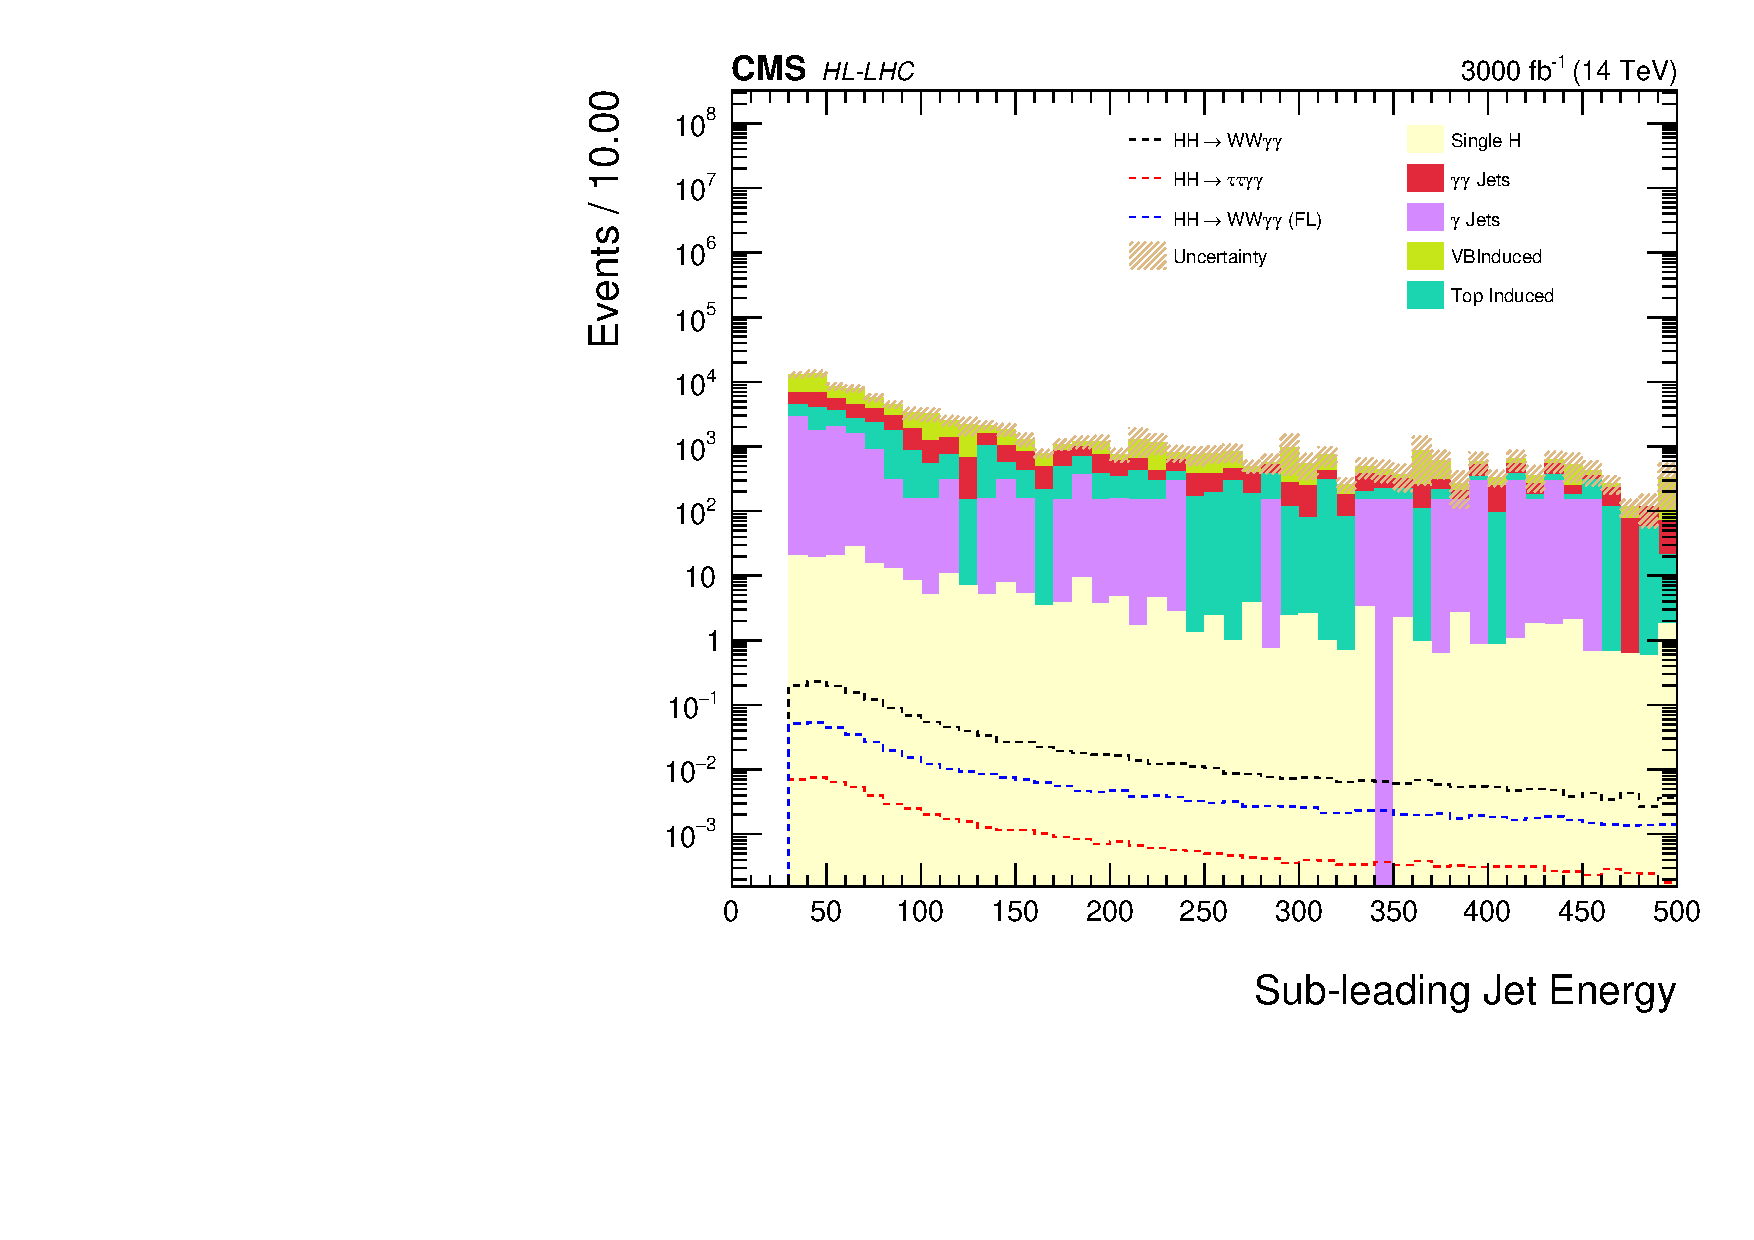
\includegraphics[width=\textwidth]{hasonel_hasTwoJ_jetE_logy.pdf}
        \vspace{-0.5cm}
        \firstsubcaption{Sub-leading jet energy}
    \end{subfigure}
    \vskip\baselineskip
    \begin{subfigure}[b]{0.475\textwidth}   
        \centering 
        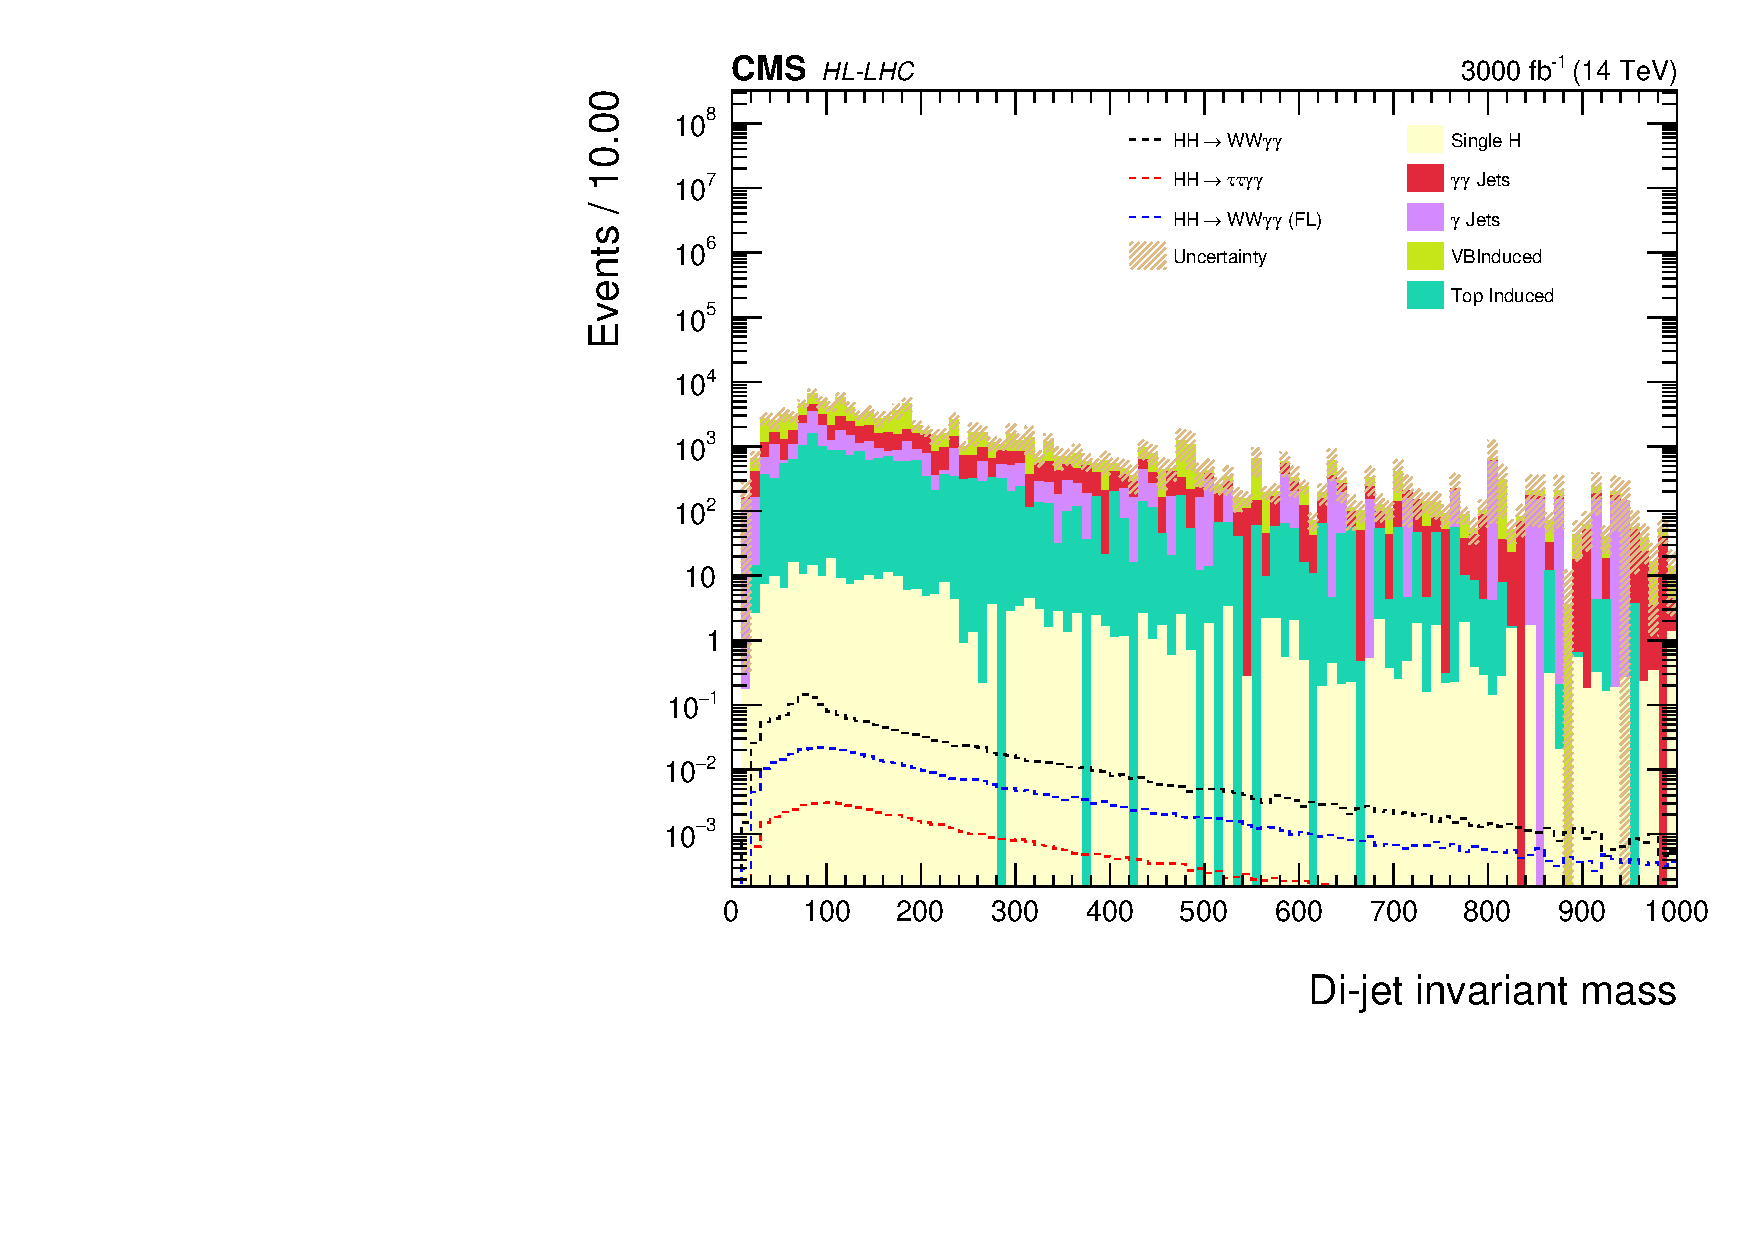
\includegraphics[width=\textwidth]{hasonel_hastwoJ_mjj_logy.pdf}
        \vspace{-0.5cm}
        \firstsubcaption{$m_{j_0,j_1}$}
    \end{subfigure}
    \hfill
    \begin{subfigure}[b]{0.475\textwidth}   
        \centering 
        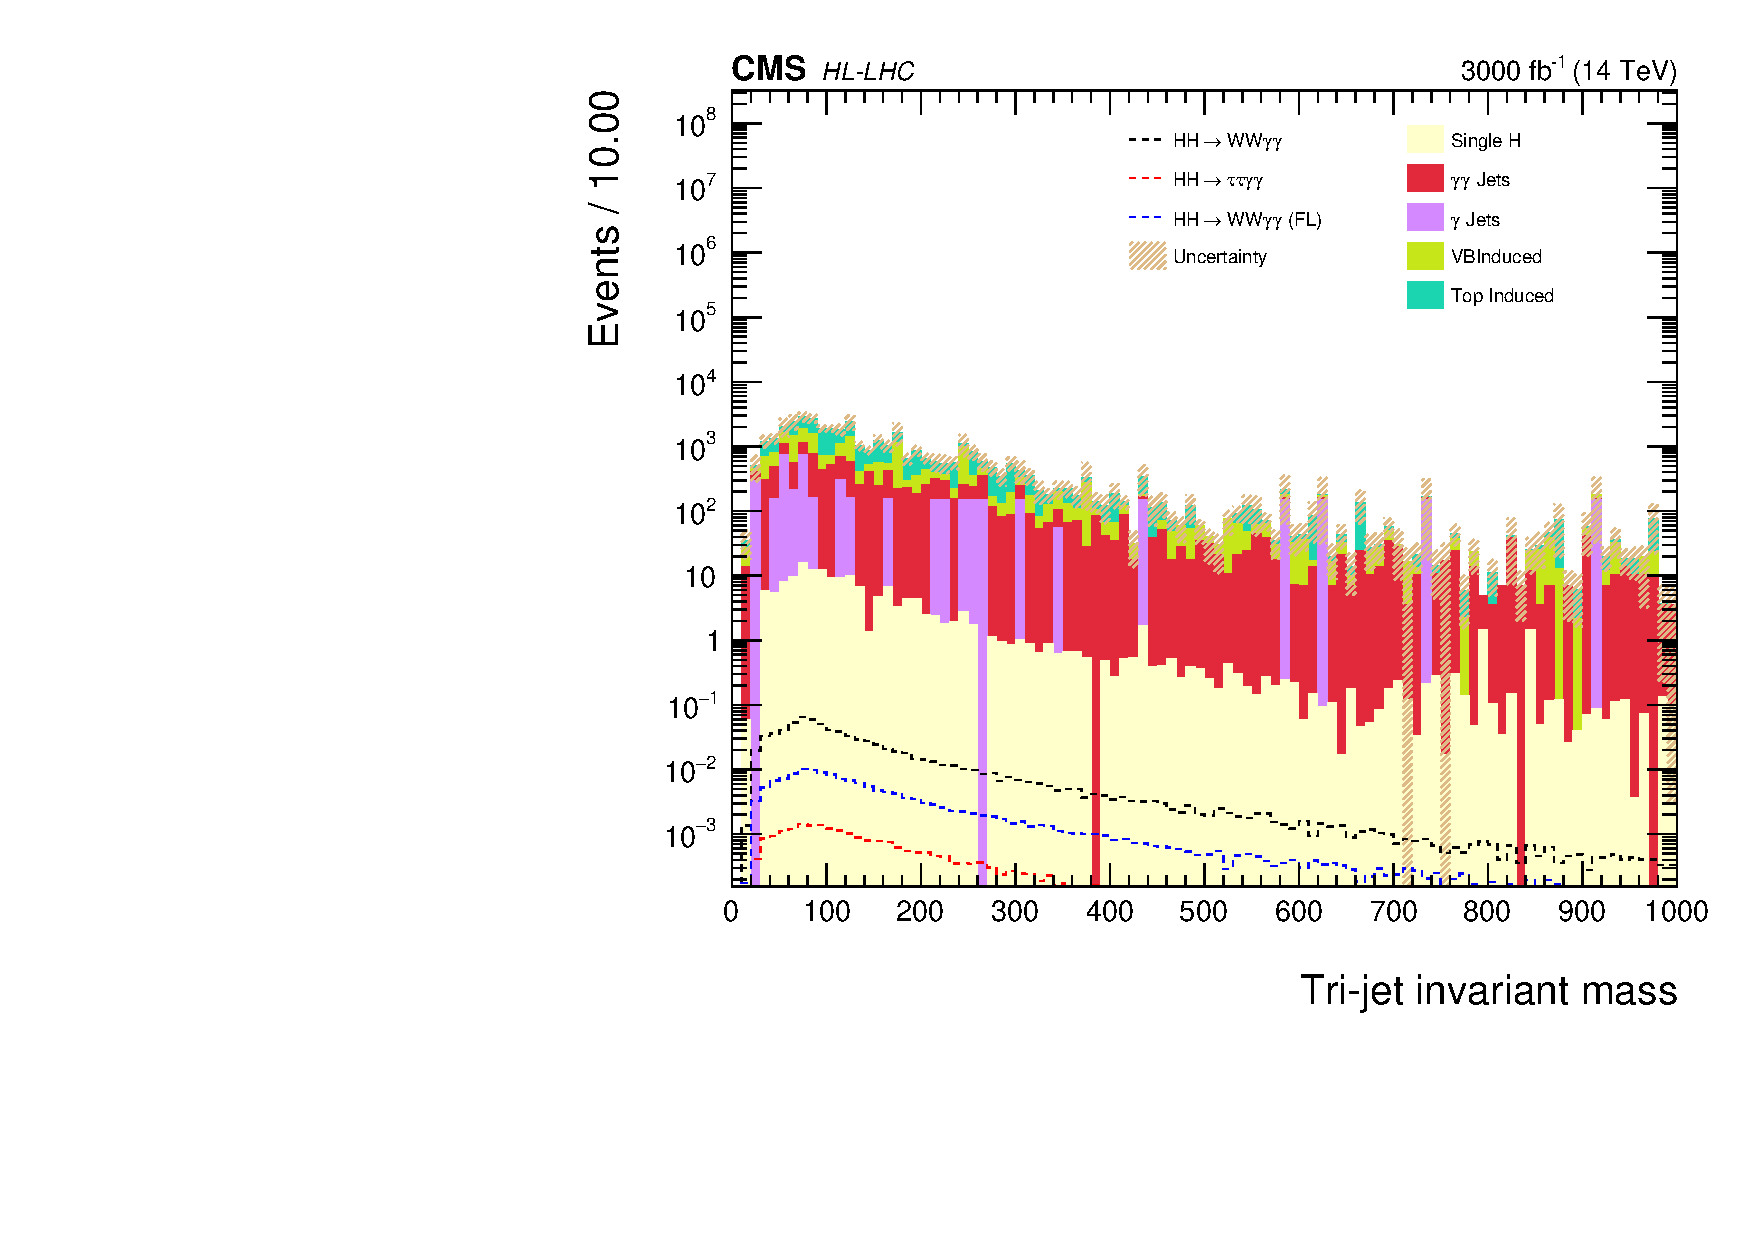
\includegraphics[width=\textwidth]{hasonel_hasthreeJ_mjj_logy.pdf}
        \vspace{-0.5cm}
        \firstsubcaption{$m_{j_1,j_2}$}
    \end{subfigure}
    \vskip\baselineskip
    \begin{subfigure}[b]{0.475\textwidth}   
        \centering 
        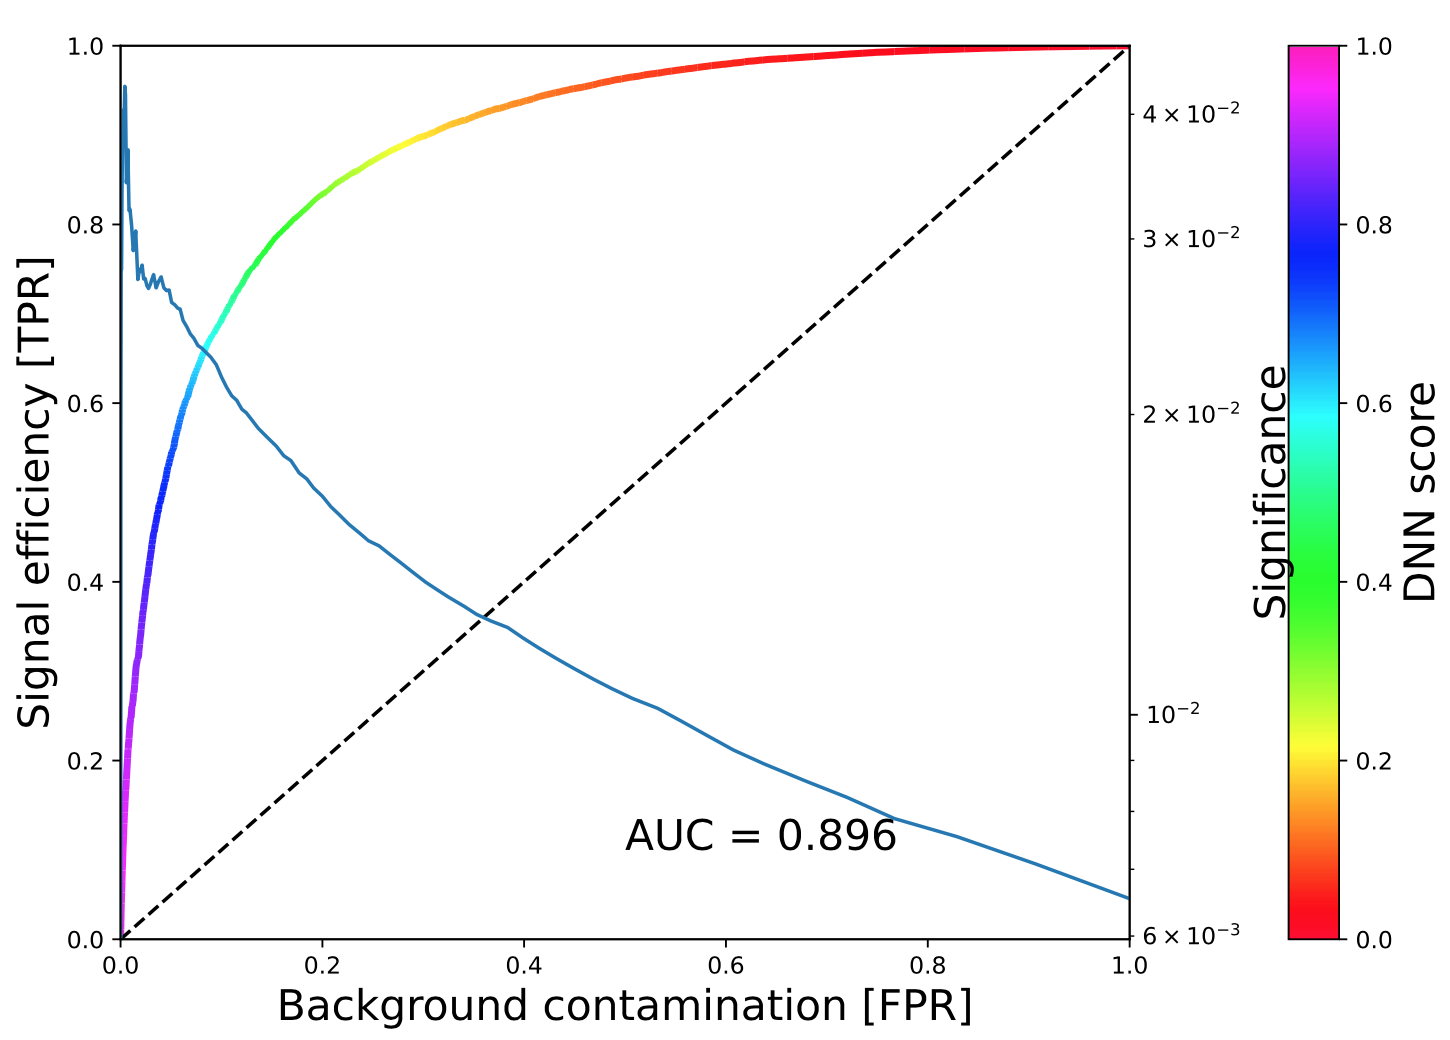
\includegraphics[width=\textwidth]{SLodd_training_roc.png}
        \vspace{-0.5cm}
        \firstsubcaption{Odd training}
    \end{subfigure}
    \hfill
    \begin{subfigure}[b]{0.475\textwidth}   
        \centering 
        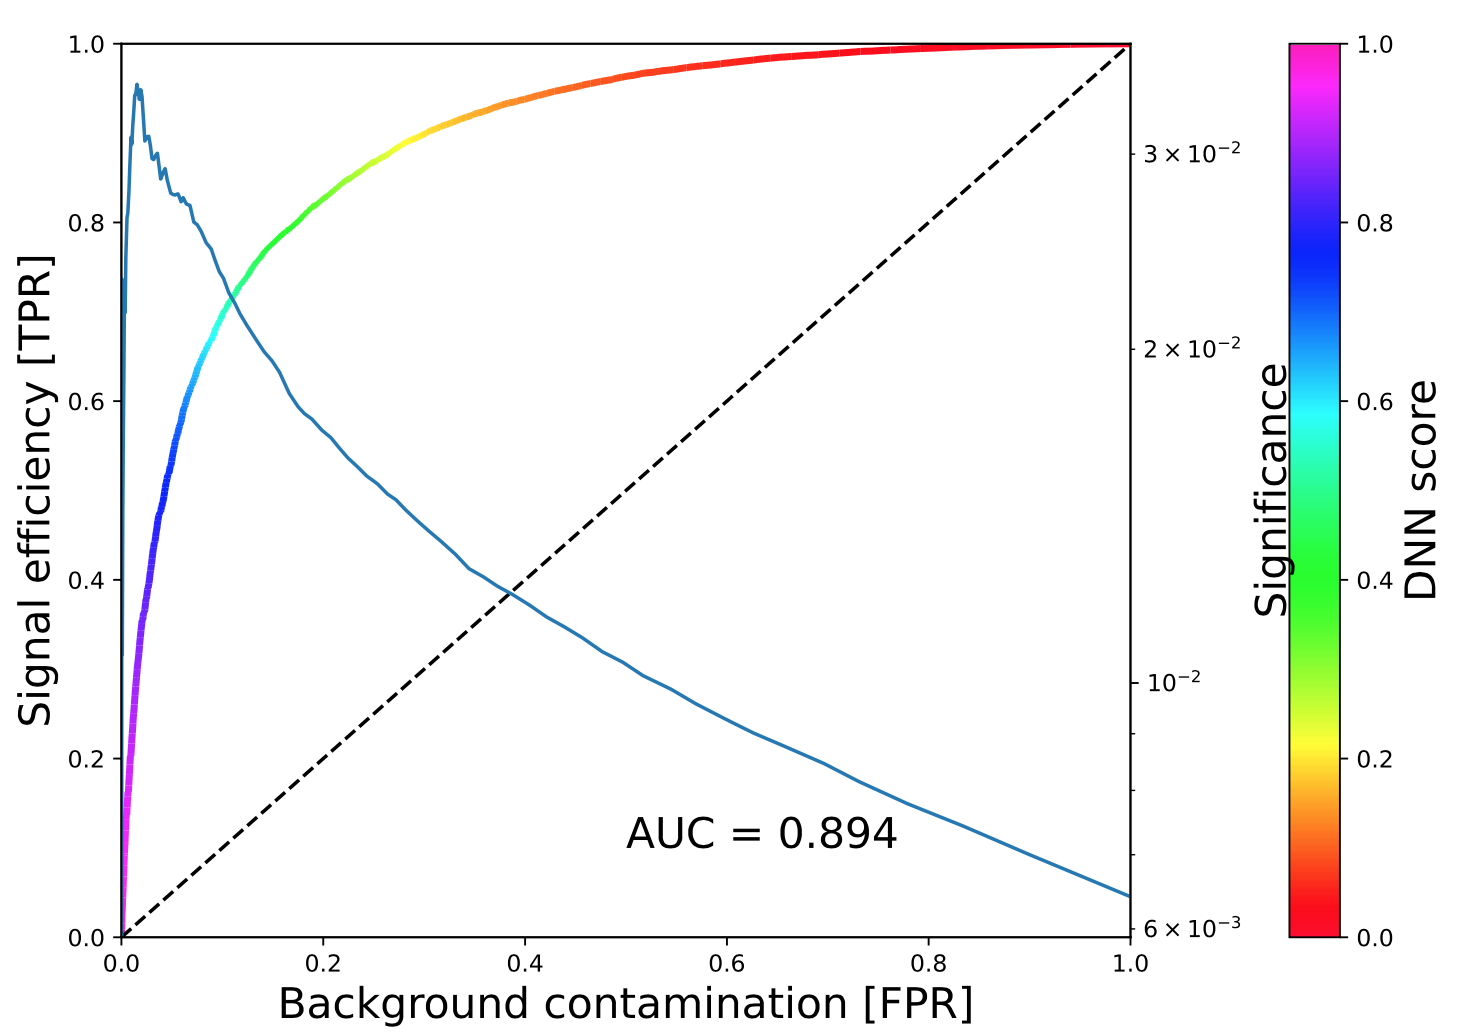
\includegraphics[width=\textwidth]{SLeven_training_roc.png}
        \vspace{-0.5cm} 
        \firstsubcaption{Even training}   
    \end{subfigure}
    \caption{\small DNN input distributions (a,b,c,d) and the ROC curves (e,f) for the semi-leptonic channel of $HH\rightarrow{WW\gamma\gamma}$ (continued).} 
\end{figure*}

\begin{figure*}[h!]
    \centering
    \begin{subfigure}[b]{0.475\textwidth}
        \centering
        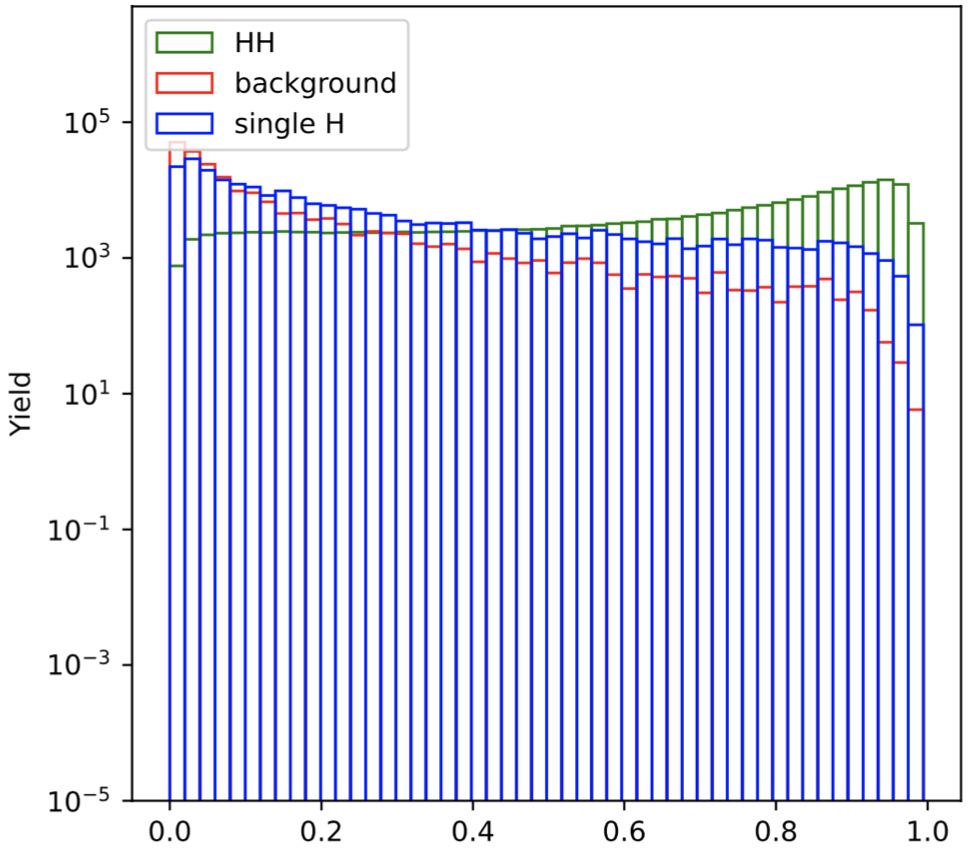
\includegraphics[width=\textwidth]{SLodd-weights.png}
        \vspace{-0.5cm}
        \firstsubcaption{Odd training}
    \end{subfigure}
    \hfill
    \begin{subfigure}[b]{0.475\textwidth}  
        \centering 
        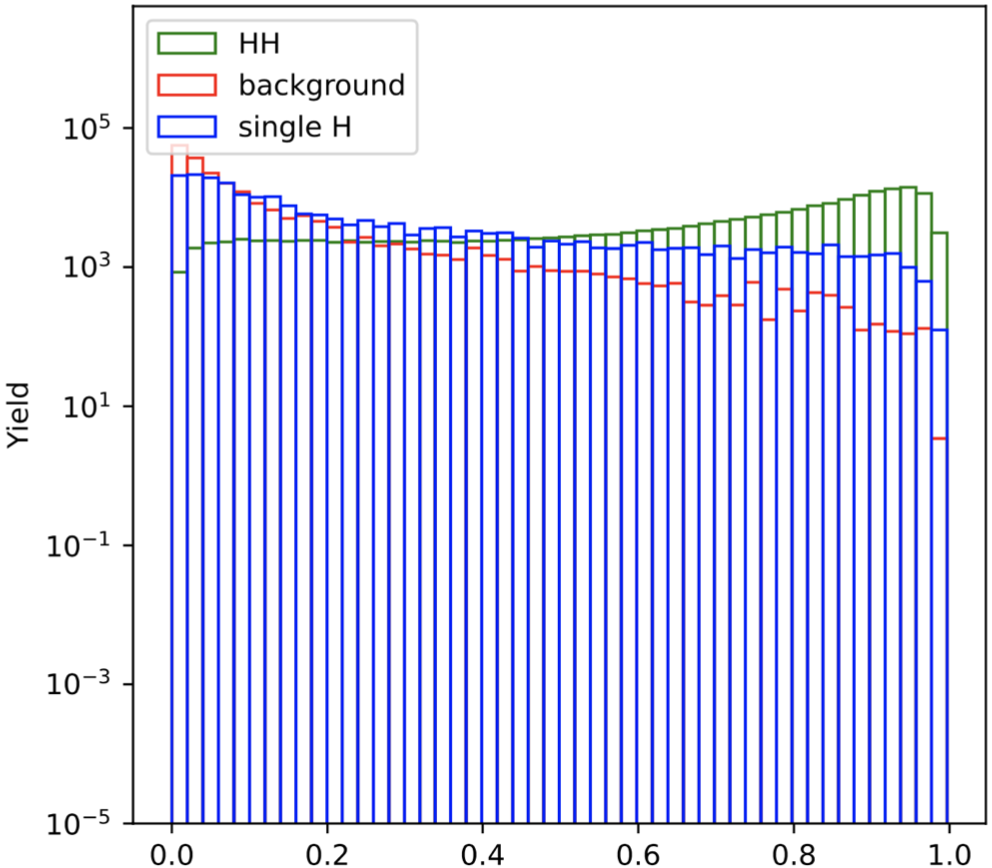
\includegraphics[width=\textwidth]{SLeven-weights.png}
        \vspace{-0.5cm}
        \firstsubcaption{Even training}
    \end{subfigure}
    \caption{\small DNN evaluations for the semi-leptonic channel of $HH\rightarrow{WW\gamma\gamma}$.} 
\end{figure*}

%%%%%%%%%%%%%%%%%%%%%%%%%%%%%%%%%%%%%%%%%%%%%%%%%%%%
%%%%%%%%%%%%%%%%%%%%%%%%%%%%%%%%%%%%%%%%%%%%%%%%%%%%
%%%%%%%%%%%%%%%%%%%%%%%%%%%%%%%%%%%%%%%%%%%%%%%%%%%%

\section*{APPENDIX A.3}
\vglue6pt

\begin{table}[h!]
    \centering
    \caption{Cut-flow report showing number of events, before selections, in the semi-leptonic channel and in its categories. Percentages in brackets show the total selection efficiency.}
\begin{tabular}{ |l|c|c| }
    \hline
    Samples                                & No selection & Fully-leptonic final state               \\
    \hline
           $HH \rightarrow WW\gamma\gamma$ &  $4.69e+01$  &  $2.14e-02$ (0.046\%) \\
      $HH \rightarrow WW\gamma\gamma (FL)$ &  $1.12e+01$  &  $3.25e-01$ (2.911\%) \\
     $HH \rightarrow \tau\tau\gamma\gamma$ &  $3.13e+00$  &  $1.64e-02$ (0.525\%) \\
     $HH \rightarrow WW \gamma\gamma (FH)$ &  $4.85e+01$  &  $4.79e-04$ (0.001\%) \\
                           \textbf{Signal} &  $1.10e+02$  &  $3.63e-01$ (0.331\%) \\
            $GGH \rightarrow \gamma\gamma$ &  $3.44e+05$  &  $0.00e+00$ (0.000\%) \\
           $VBFH \rightarrow \gamma\gamma$ &  $2.85e+04$  &  $5.38e-02$ (0.000\%) \\
            $ttH \rightarrow \gamma\gamma$ &  $4.18e+03$  &  $2.39e+00$ (0.057\%) \\
             $VH \rightarrow \gamma\gamma$ &  $1.63e+04$  &  $3.03e+00$ (0.019\%) \\
                                     $THQ$ &  $6.16e+02$  &  $7.81e-02$ (0.013\%) \\
              $\gamma\gamma + jets 80-Inf$ &  $2.96e+08$  &  $2.87e+02$ (0.000\%) \\
               $\gamma\gamma + jets 40-80$ &  $9.98e+08$  &  $0.00e+00$ (0.000\%) \\
                                  $G+jets$ &  $2.99e+09$  &  $0.00e+00$ (0.000\%) \\
                         $G+jets 20-40GeV$ &  $7.83e+08$  &  $0.00e+00$ (0.000\%) \\
                           $G+jets 20-Inf$ &  $1.17e+10$  &  $0.00e+00$ (0.000\%) \\
                 $W1Jets \rightarrow L\nu$ &  $3.11e+10$  &  $0.00e+00$ (0.000\%) \\
                 $W2Jets \rightarrow L\nu$ &  $8.90e+09$  &  $0.00e+00$ (0.000\%) \\
                 $W3Jets \rightarrow L\nu$ &  $3.80e+09$  &  $0.00e+00$ (0.000\%) \\
                                    $WGJJ$ &  $1.81e+07$  &  $1.00e+01$ (0.000\%) \\
                                 $WGGJets$ &  $5.65e+06$  &  $5.70e+00$ (0.000\%) \\
                                  $DYJets$ &  $1.71e+10$  &  $0.00e+00$ (0.000\%) \\
                                      $ZG$ &  $4.36e+08$  &  $6.20e+02$ (0.000\%) \\
                           $WW(inclusive)$ &  $2.11e+08$  &  $1.91e+01$ (0.000\%) \\
                    $t\bar{t} (inclusive)$ &  $2.59e+09$  &  $5.25e+01$ (0.000\%) \\
                                 $ttGJets$ &  $1.37e+07$  &  $7.83e+01$ (0.001\%) \\
                                    $ttGG$ &  $5.59e+04$  &  $4.89e+00$ (0.009\%) \\
                                     $ttW$ &  $6.76e+05$  &  $2.52e-01$ (0.000\%) \\
                       \textbf{Background} &  $8.10e+10$  &  $1.08e+03$ (0.000\%) \\
    \hline
\end{tabular}
\label{fullyleptonic-cutflow}
\end{table}

%%%%%%%%%%%%%%%%%%%%%%%%%%%%%%%%%%%%%%%%%%%%%%%%%%%%
%%%%%%%%%%%%%%%%%%%%%%%%%%%%%%%%%%%%%%%%%%%%%%%%%%%%
%%%%%%%%%%%%%%%%%%%%%%%%%%%%%%%%%%%%%%%%%%%%%%%%%%%%

\section*{APPENDIX A.4}
\vglue6pt

\begin{table}[h!]
    \caption{Input variables used to train 1$\tau$ final state DNN.}
    \resizebox{\textwidth}{!}{
    \begin{tabular}{ l | l }
    \hline
    Feature & Description \\
    \hline
    Leading Photon p$_T$ / \mgg & \pt of the leading good photon scaled to diphoton mass. \\
    Leading Photon Energy / \mgg & Energy of the leading good photon scaled to diphoton mass. \\
    Leading Photon $\eta$ & Pseudorapidity of the leading good photon \\
    Leading Photon $\phi$ & Direction in the transverse plane of the leading good photon\\
    Sub-leading Photon p$_T$ / \mgg & \pt of the sub-leading good photon scaled to diphoton mass.\\
    Sub-leading Photon Energy / \mgg & Energy of the sub-leading good photon scaled to diphoton mass. \\
    Sub-leading Photon $\eta$ & Pseudorapidity of the sub-leading good photon\\
    Sub-leading Photon $\phi$ & Direction in the transverse plane of the sub-leading good photon\\
    Leading Tau p$_T$ & \pt of the leading good Tau \\
    Leading Tau $\eta$ & Pseudorapidity of the leading good Tau \\
    Leading Tau $\phi$ & Direction in the transverse plane of the leading good Tau \\
    Leading Tau Energy & Energy of the leading good Tau \\
    Jet Multiplicity & Number of jets in the event (flavour inclusive) \\
    B-tagged jet Multiplicity & Number of b-tagged jets in the event (flavour inclusive) \\
    Leading Jet p$_T$ & \pt of the leading good jet \\
    Leading Jet $\eta$ & Pseudorapidity of the leading good jet \\
    Sub-leading Jet p$_T$ & \pt of the sub-leading good jet \\
    Sub-leading Jet $\eta$ & Pseudorapidity of the sub-leading good jet \\
    MET & Missing transverse energy in the event \\ 
    \hline
    \end{tabular}
    }
    \label{dnninputs_1tau}
\end{table}

\begin{figure*}[h!]
    \centering
    \begin{subfigure}[b]{0.475\textwidth}
        \centering
        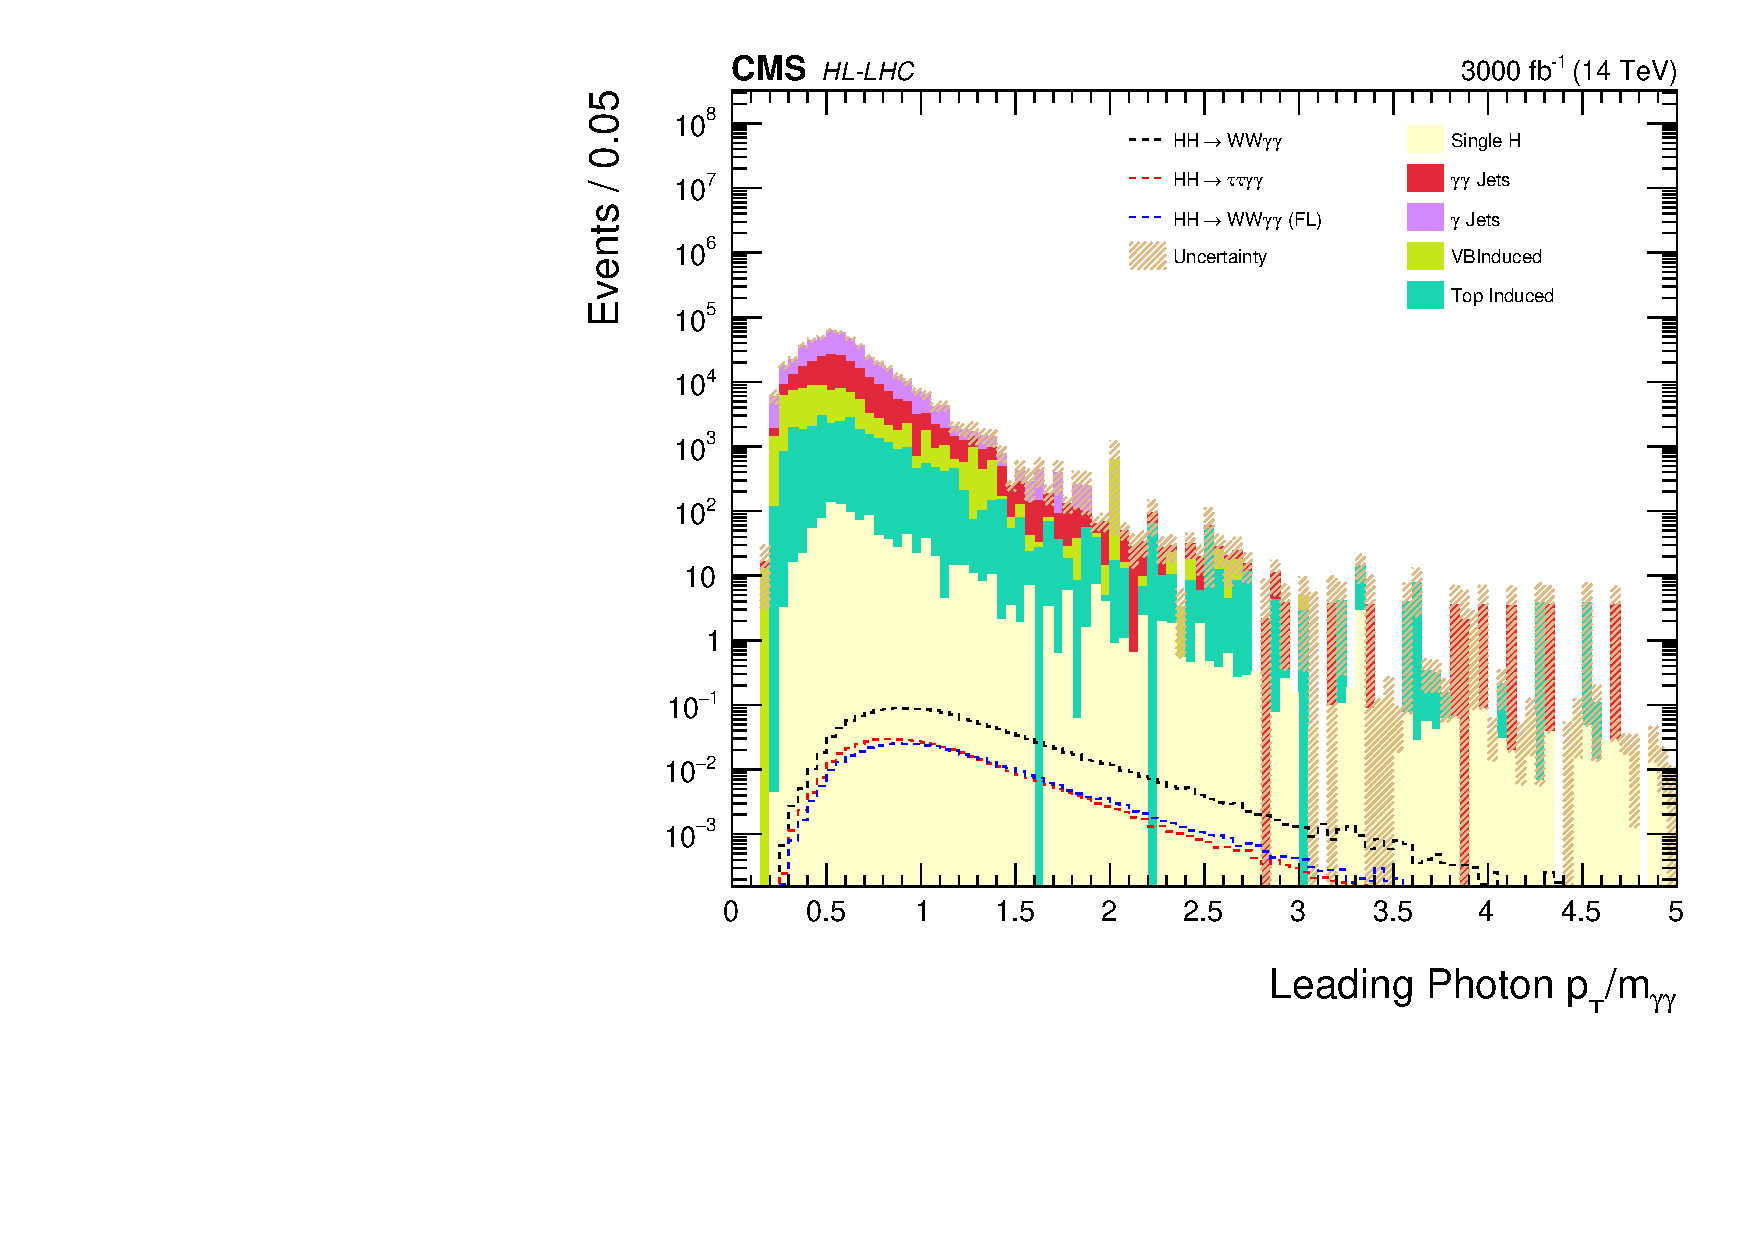
\includegraphics[width=\textwidth]{c3_pt_mgg_logy.pdf}
        \vspace{-0.5cm}
        \firstsubcaption{Leading Photon $p_{T}/m_{\gamma\gamma}$}
    \end{subfigure}
    \hfill
    \begin{subfigure}[b]{0.475\textwidth}  
        \centering 
        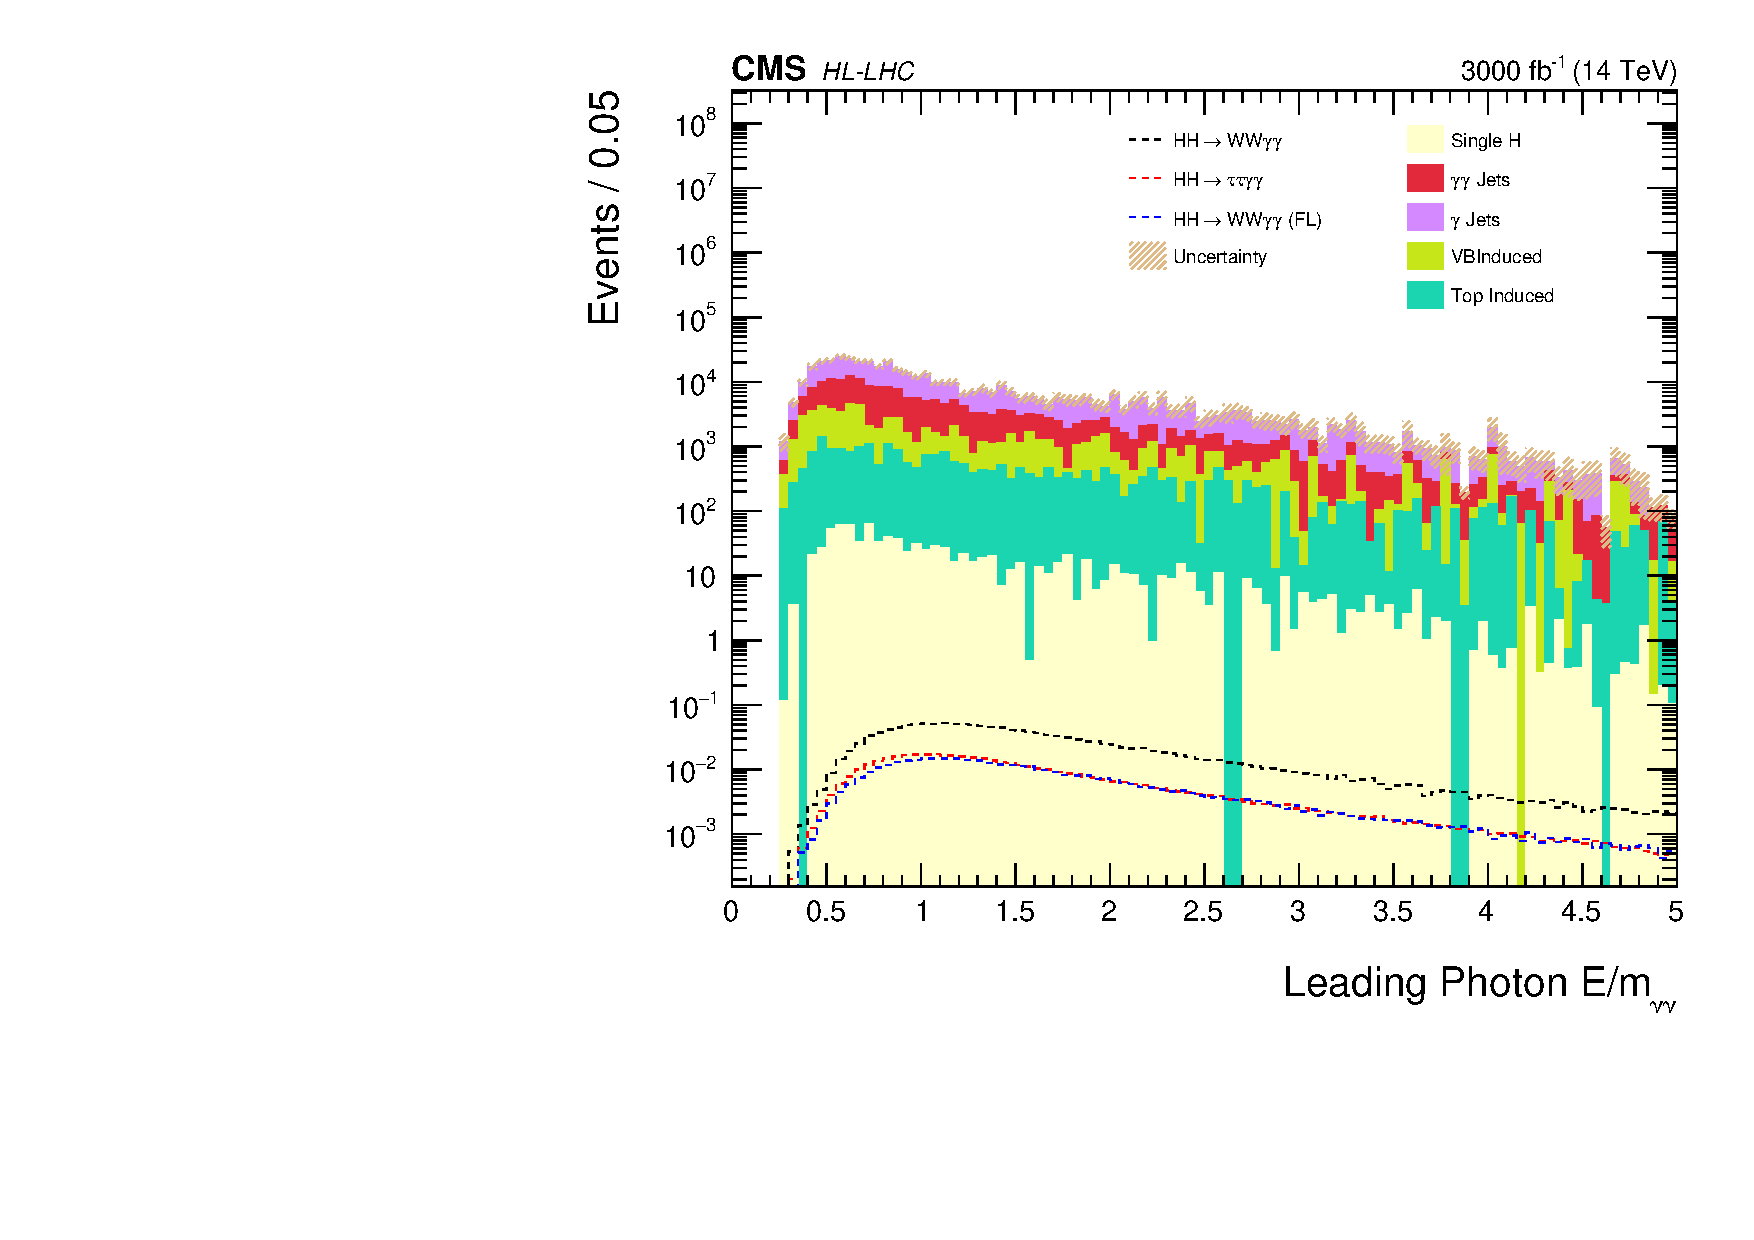
\includegraphics[width=\textwidth]{c3_LE_mgg_logy.pdf}
        \vspace{-0.5cm}
        \firstsubcaption{Leading Photon $E/m_{\gamma\gamma}$}
    \end{subfigure}
    \vskip\baselineskip
    \begin{subfigure}[b]{0.475\textwidth}   
        \centering 
        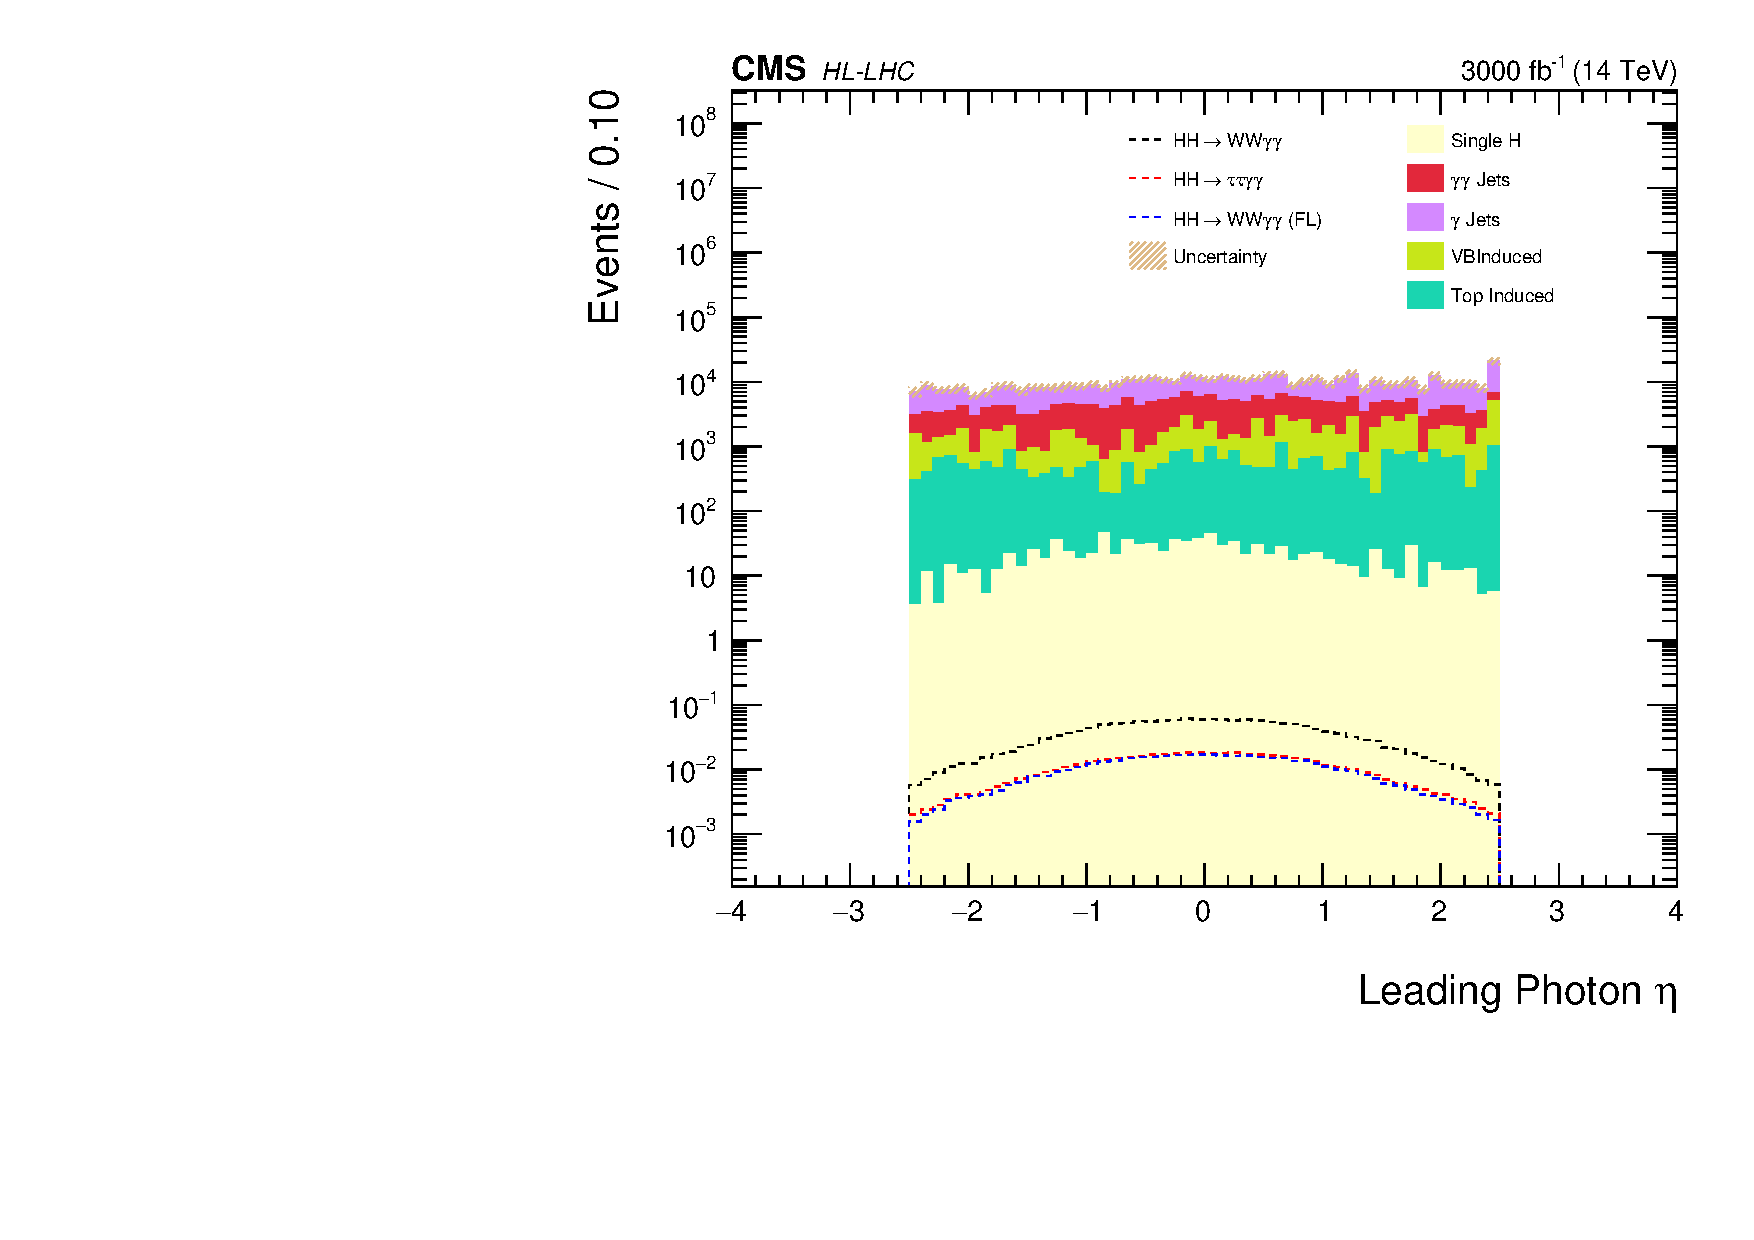
\includegraphics[width=\textwidth]{c3_leadingphoton_eta_logy.pdf}
        \vspace{-0.5cm}
        \firstsubcaption{Leading Photon $\eta$}
    \end{subfigure}
    \hfill
    \begin{subfigure}[b]{0.475\textwidth}   
        \centering 
        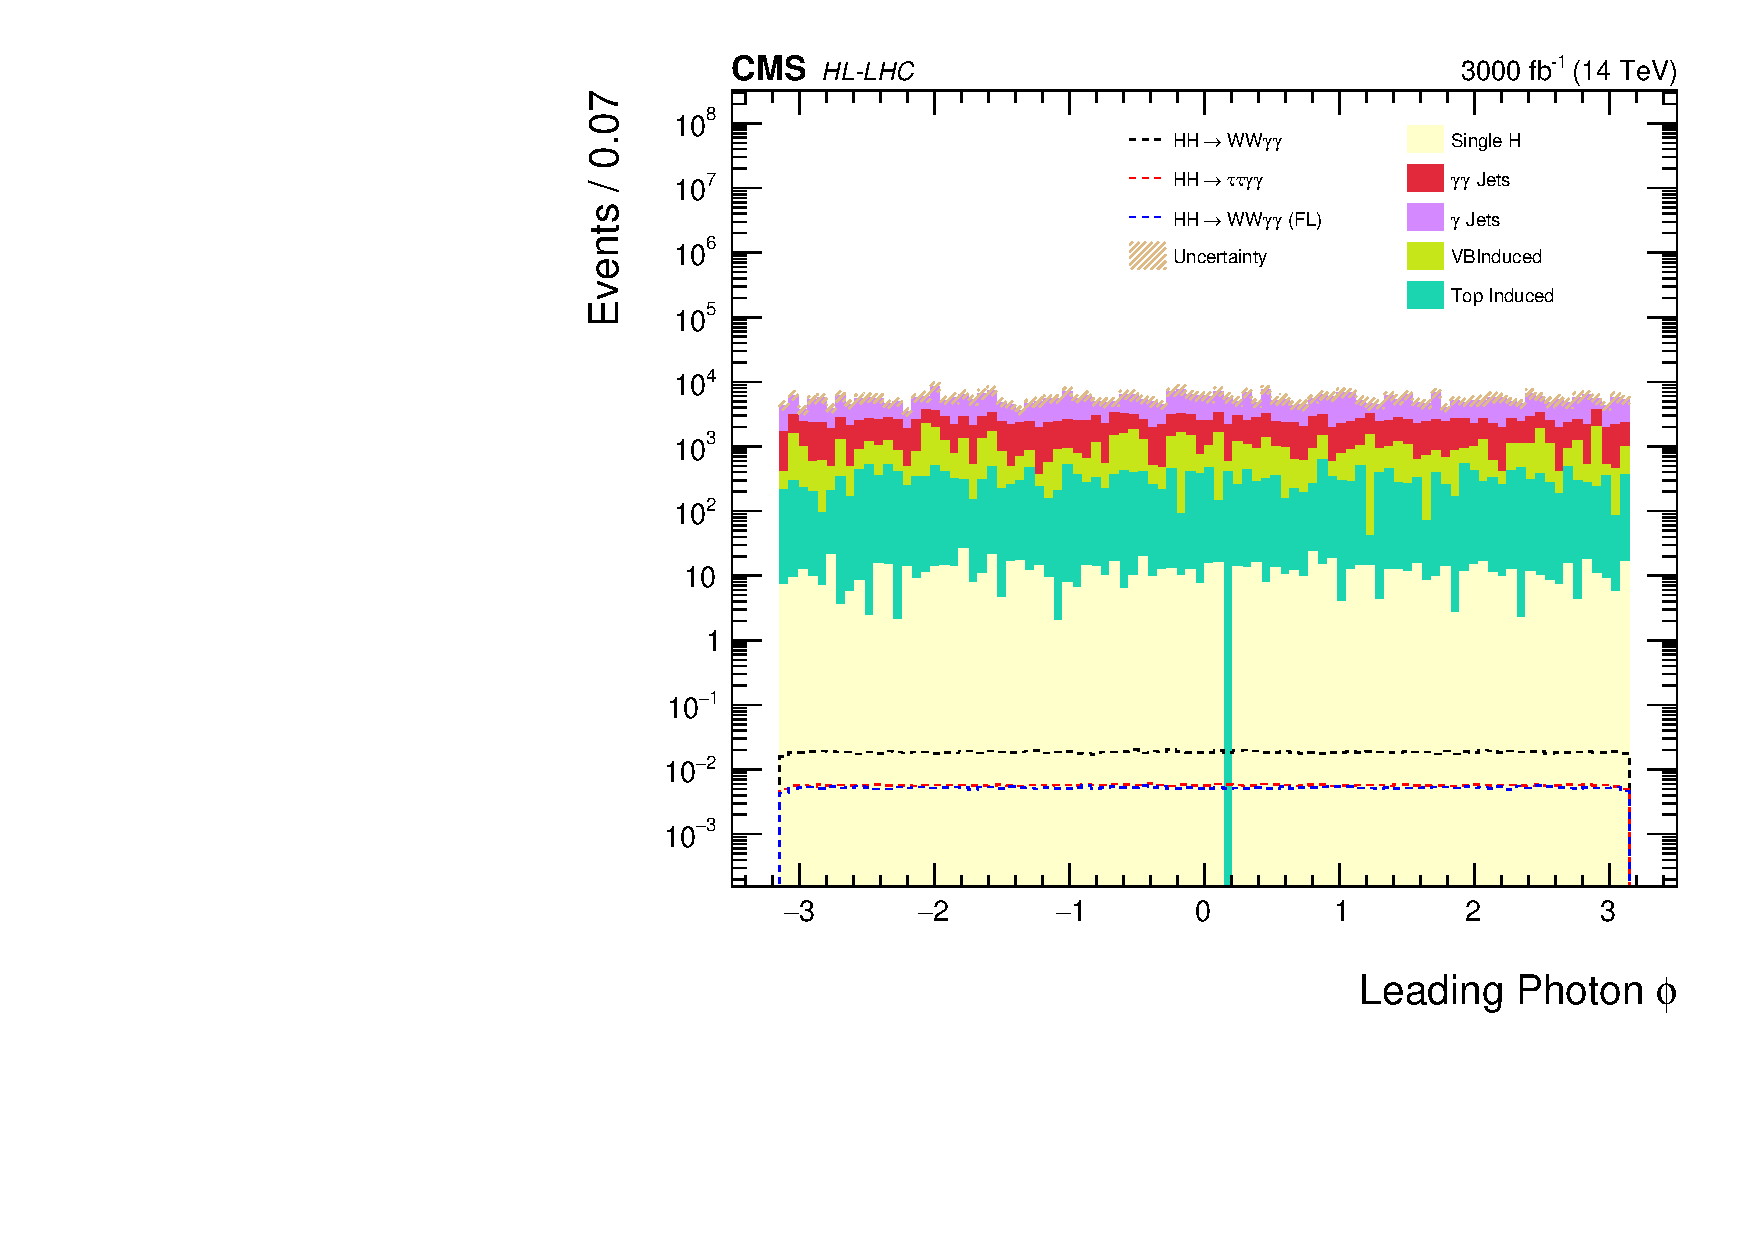
\includegraphics[width=\textwidth]{c3_leadingphoton_phi_logy.pdf}
        \vspace{-0.5cm}
        \firstsubcaption{Leading Photon $\phi$}
    \end{subfigure}
    \vskip\baselineskip
    \begin{subfigure}[b]{0.475\textwidth}   
        \centering 
        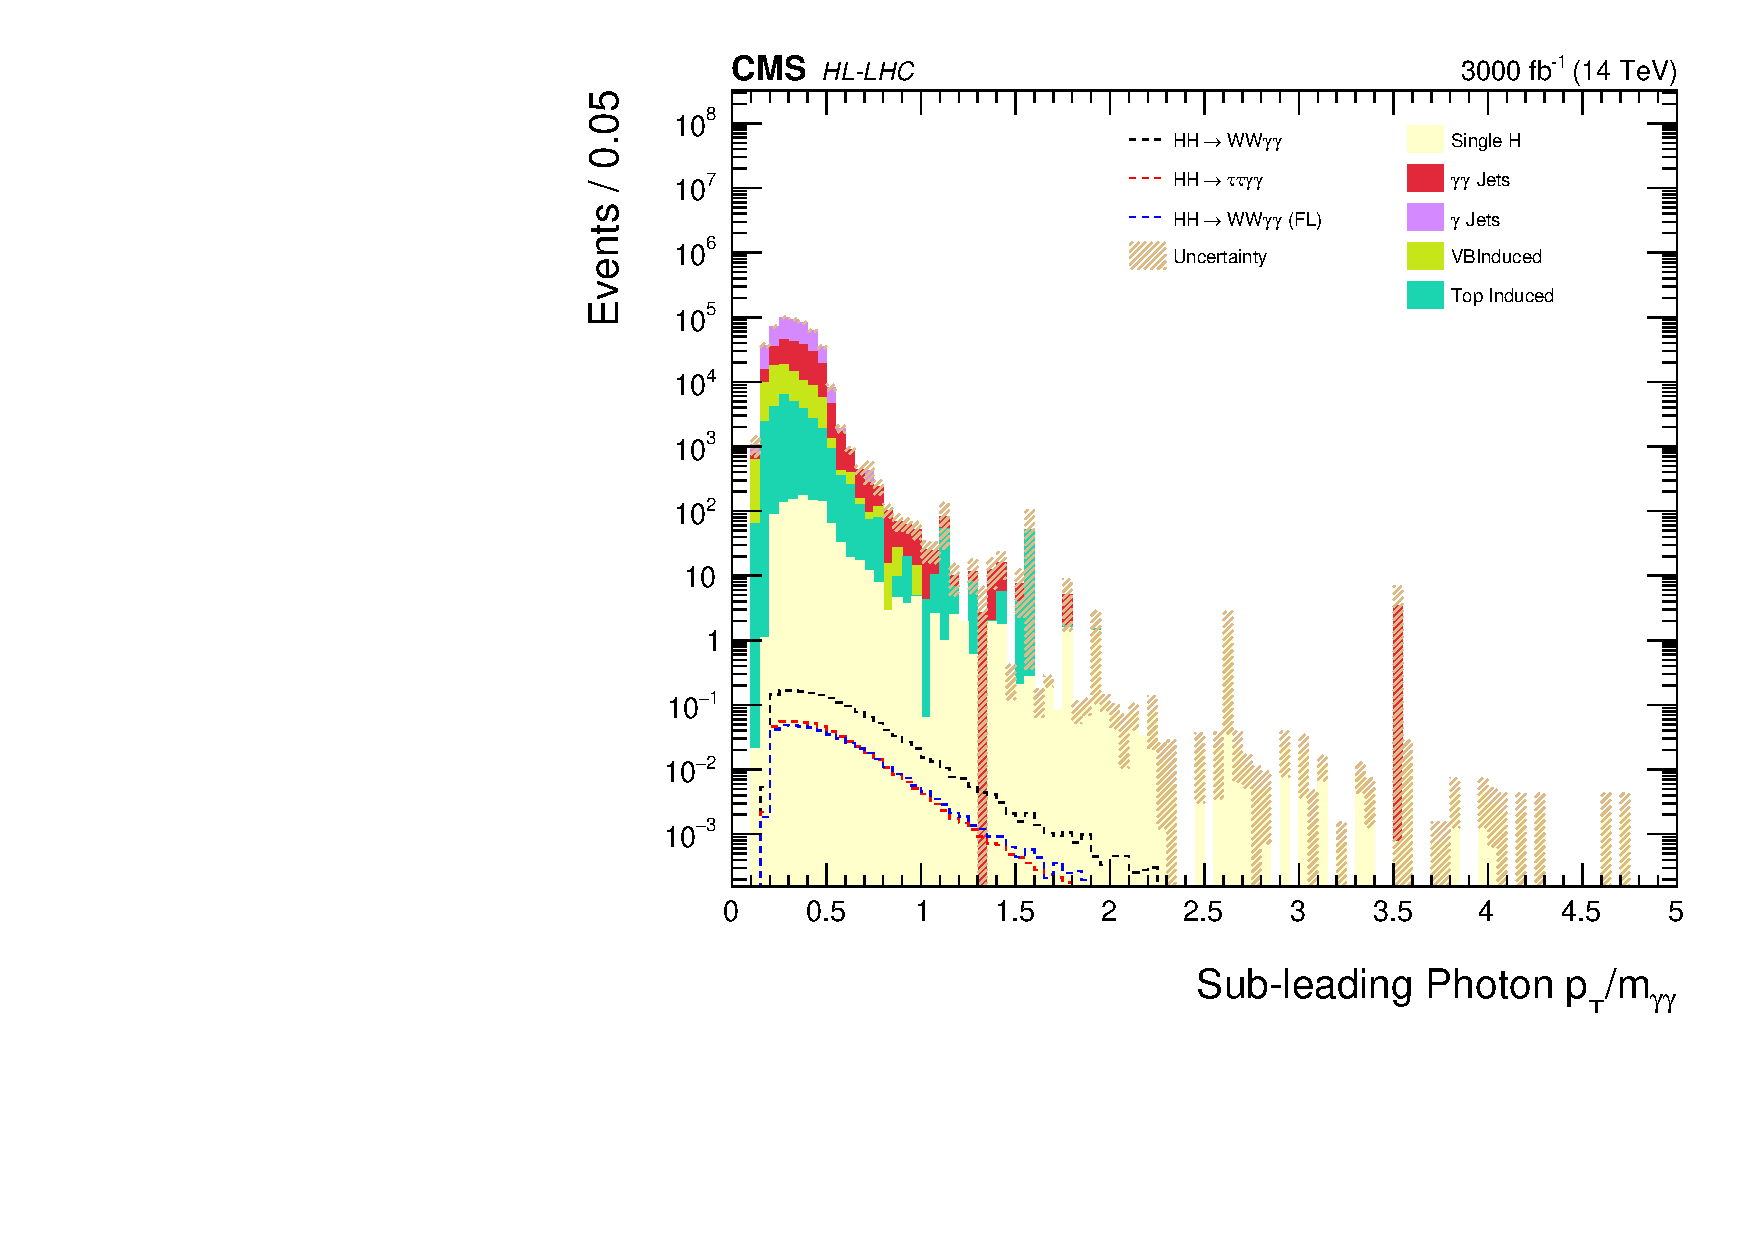
\includegraphics[width=\textwidth]{c3_SLpt_mgg_logy.pdf}
        \vspace{-0.5cm}
        \firstsubcaption{Sub-leading Photon $p_{T}/m_{\gamma\gamma}$}
    \end{subfigure}
    \hfill
    \begin{subfigure}[b]{0.475\textwidth}   
        \centering 
        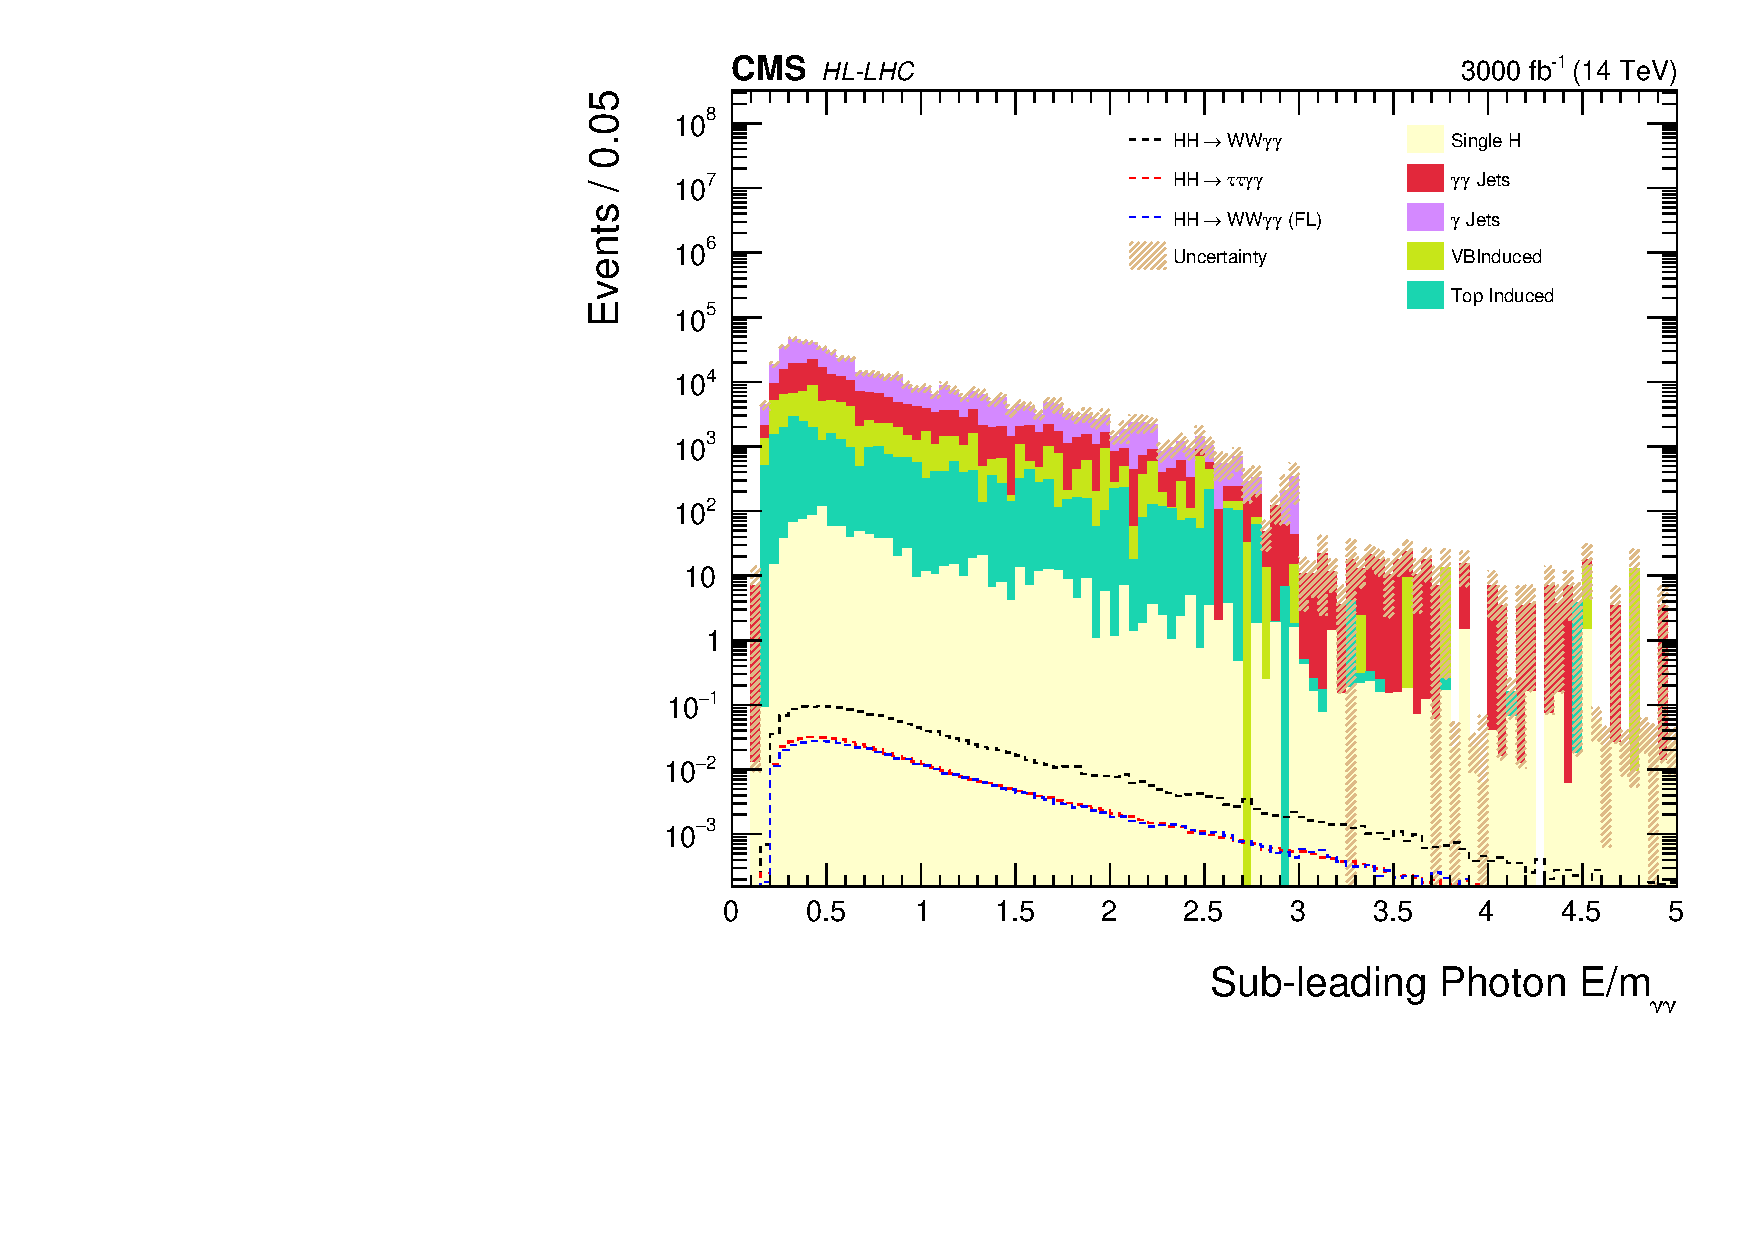
\includegraphics[width=\textwidth]{c3_SLE_mgg_logy.pdf}
        \vspace{-0.5cm}
        \firstsubcaption{Sub-leading Photon $E/m_{\gamma\gamma}$}   
    \end{subfigure}
    \caption{\small DNN input distributions for the 1$\tau$ channel of $HH\rightarrow{\tau\tau\gamma\gamma}$ (continued).}
    \label{dnninputDists_tau}
\end{figure*}

\begin{figure*}[h!]
    \centering
    \begin{subfigure}[b]{0.475\textwidth}
        \centering
        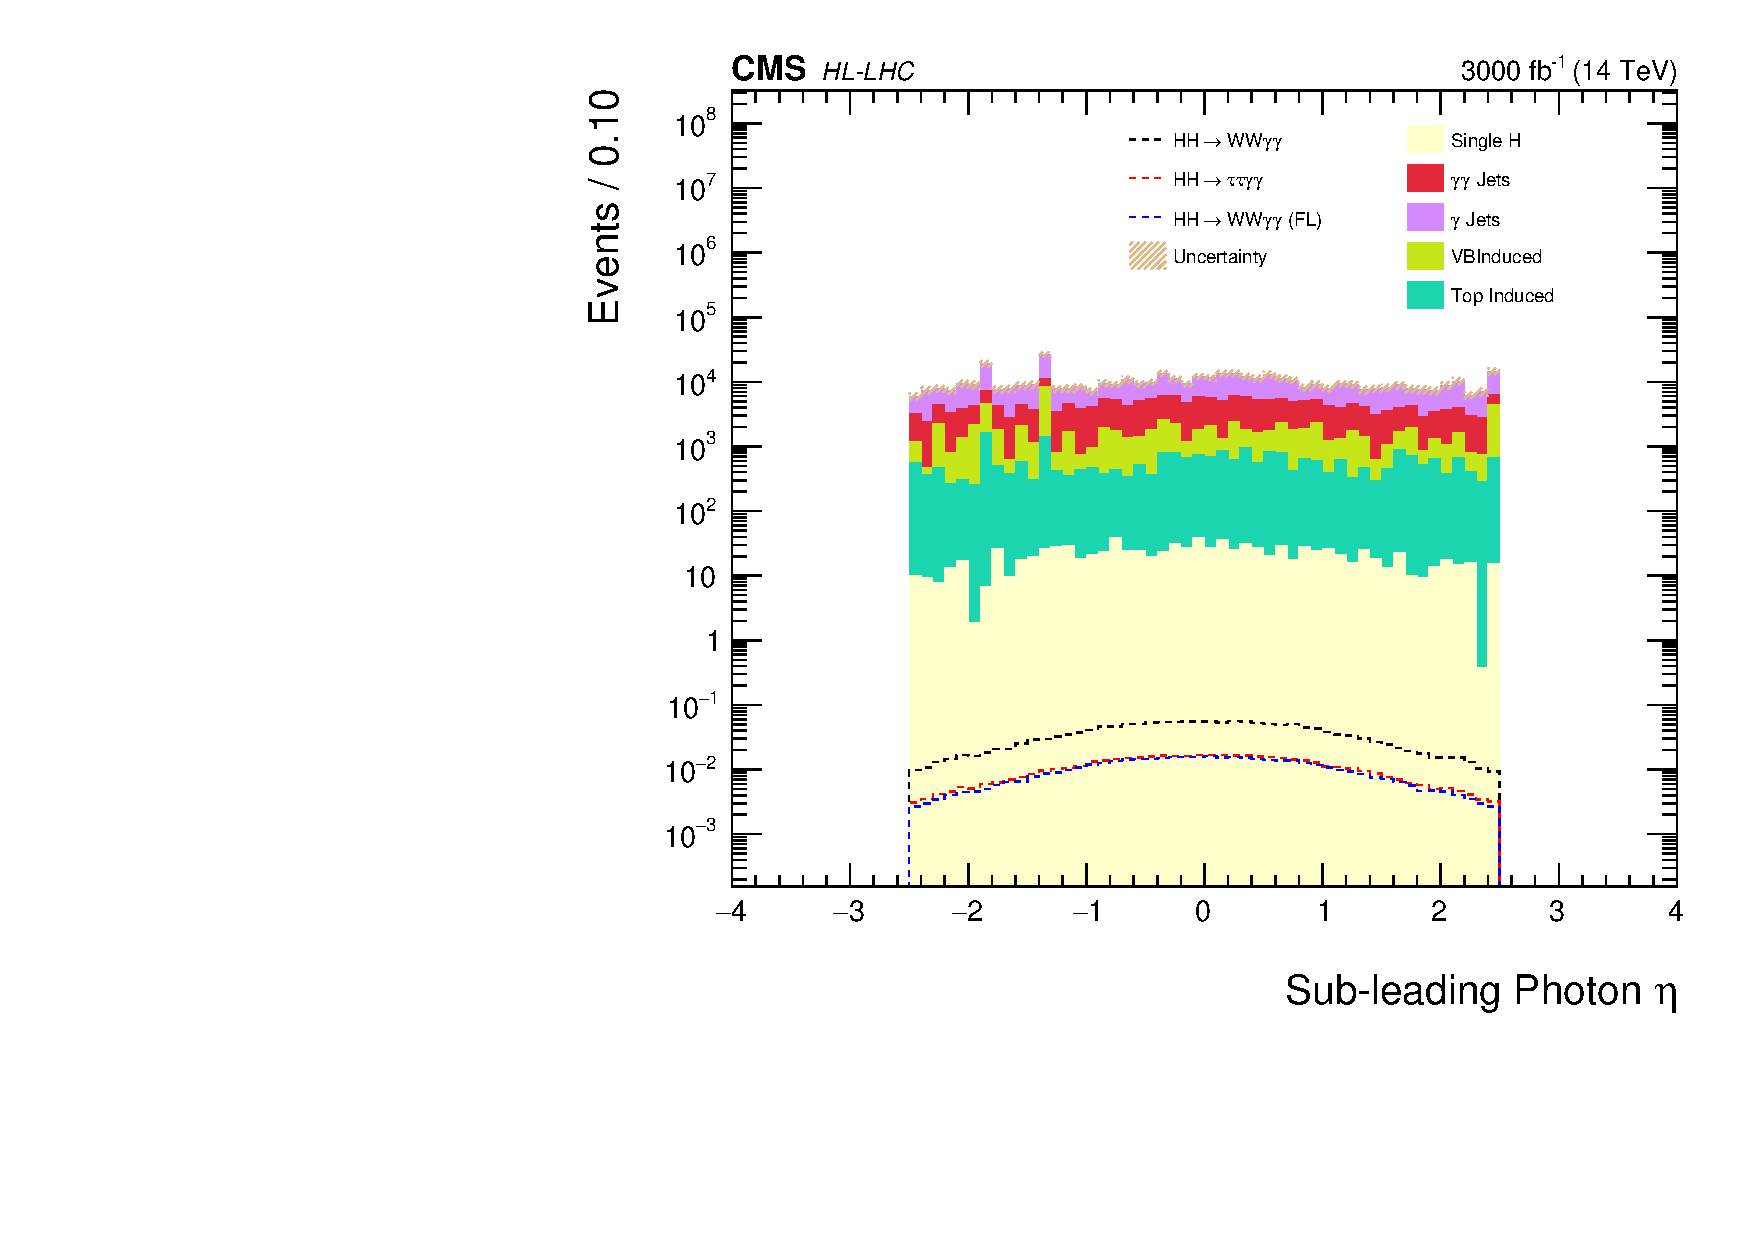
\includegraphics[width=\textwidth]{c3_subleadingphoton_eta_logy.pdf}
        \vspace{-0.5cm}
        \firstsubcaption{Sub-leading Photon $\eta$}
    \end{subfigure}
    \hfill
    \begin{subfigure}[b]{0.475\textwidth}  
        \centering 
        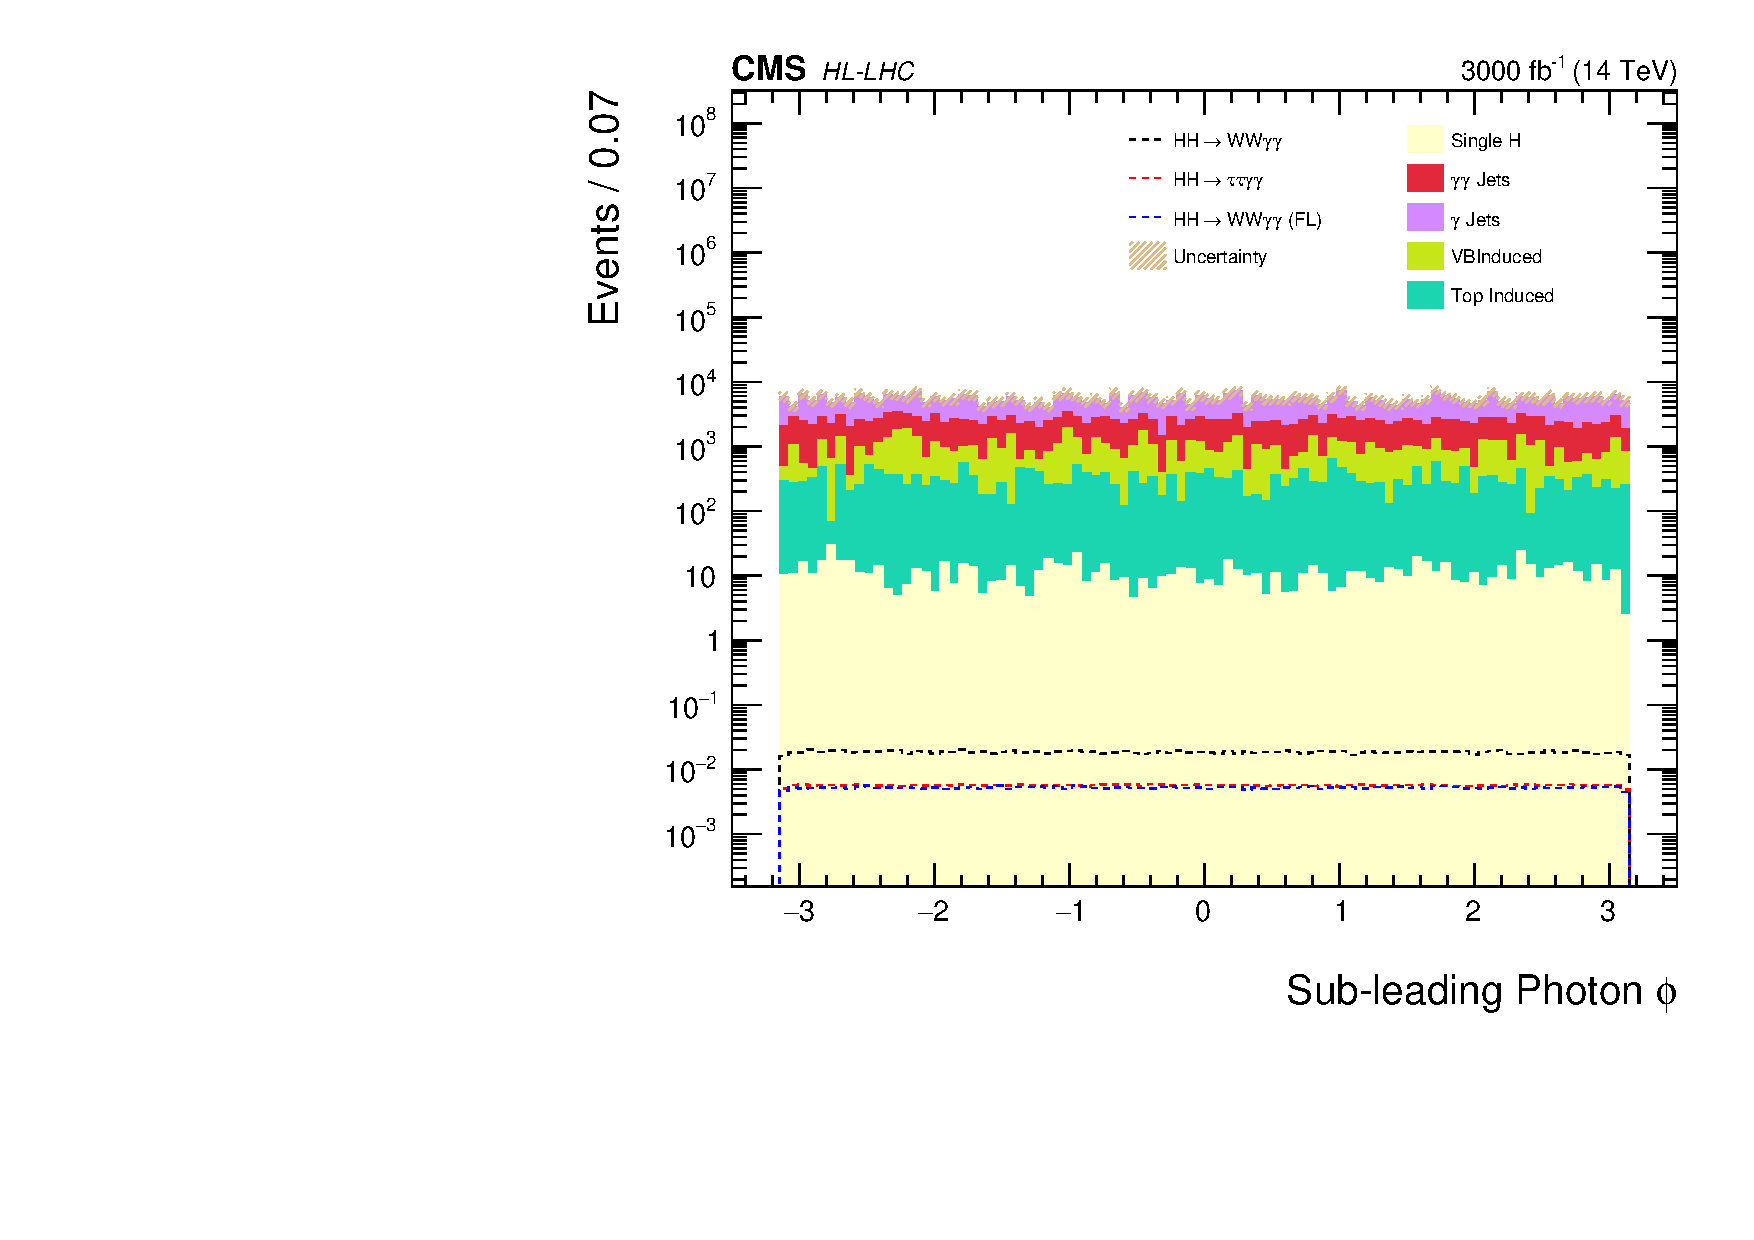
\includegraphics[width=\textwidth]{c3_subleadingphoton_phi_logy.pdf}
        \vspace{-0.5cm}
        \firstsubcaption{Sub-leading Photon $\phi$}
    \end{subfigure}
    \vskip\baselineskip
    \begin{subfigure}[b]{0.475\textwidth}   
        \centering 
        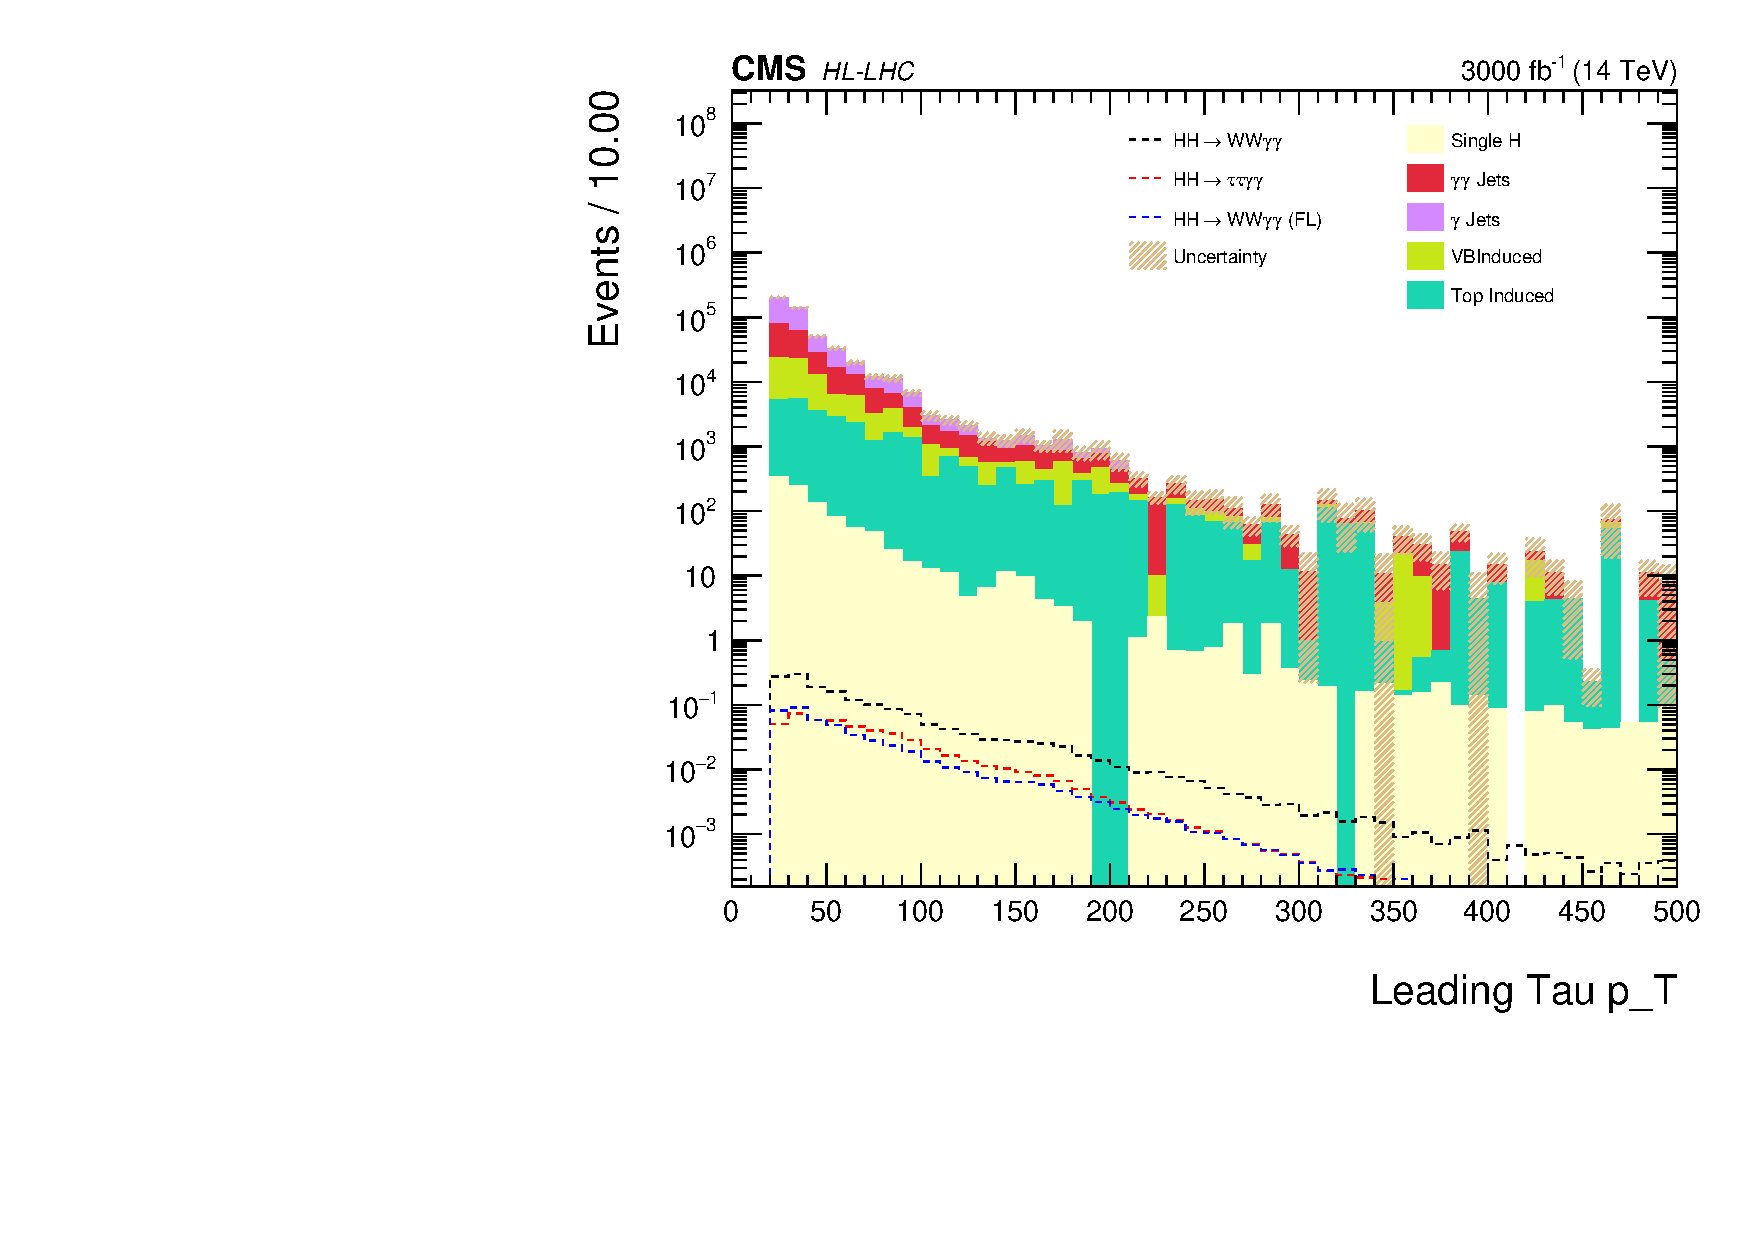
\includegraphics[width=\textwidth]{c3_leadingtau_pt_logy.pdf}
        \vspace{-0.5cm}
        \firstsubcaption{Leading Tau \pt}
    \end{subfigure}
    \hfill
    \begin{subfigure}[b]{0.475\textwidth}   
        \centering 
        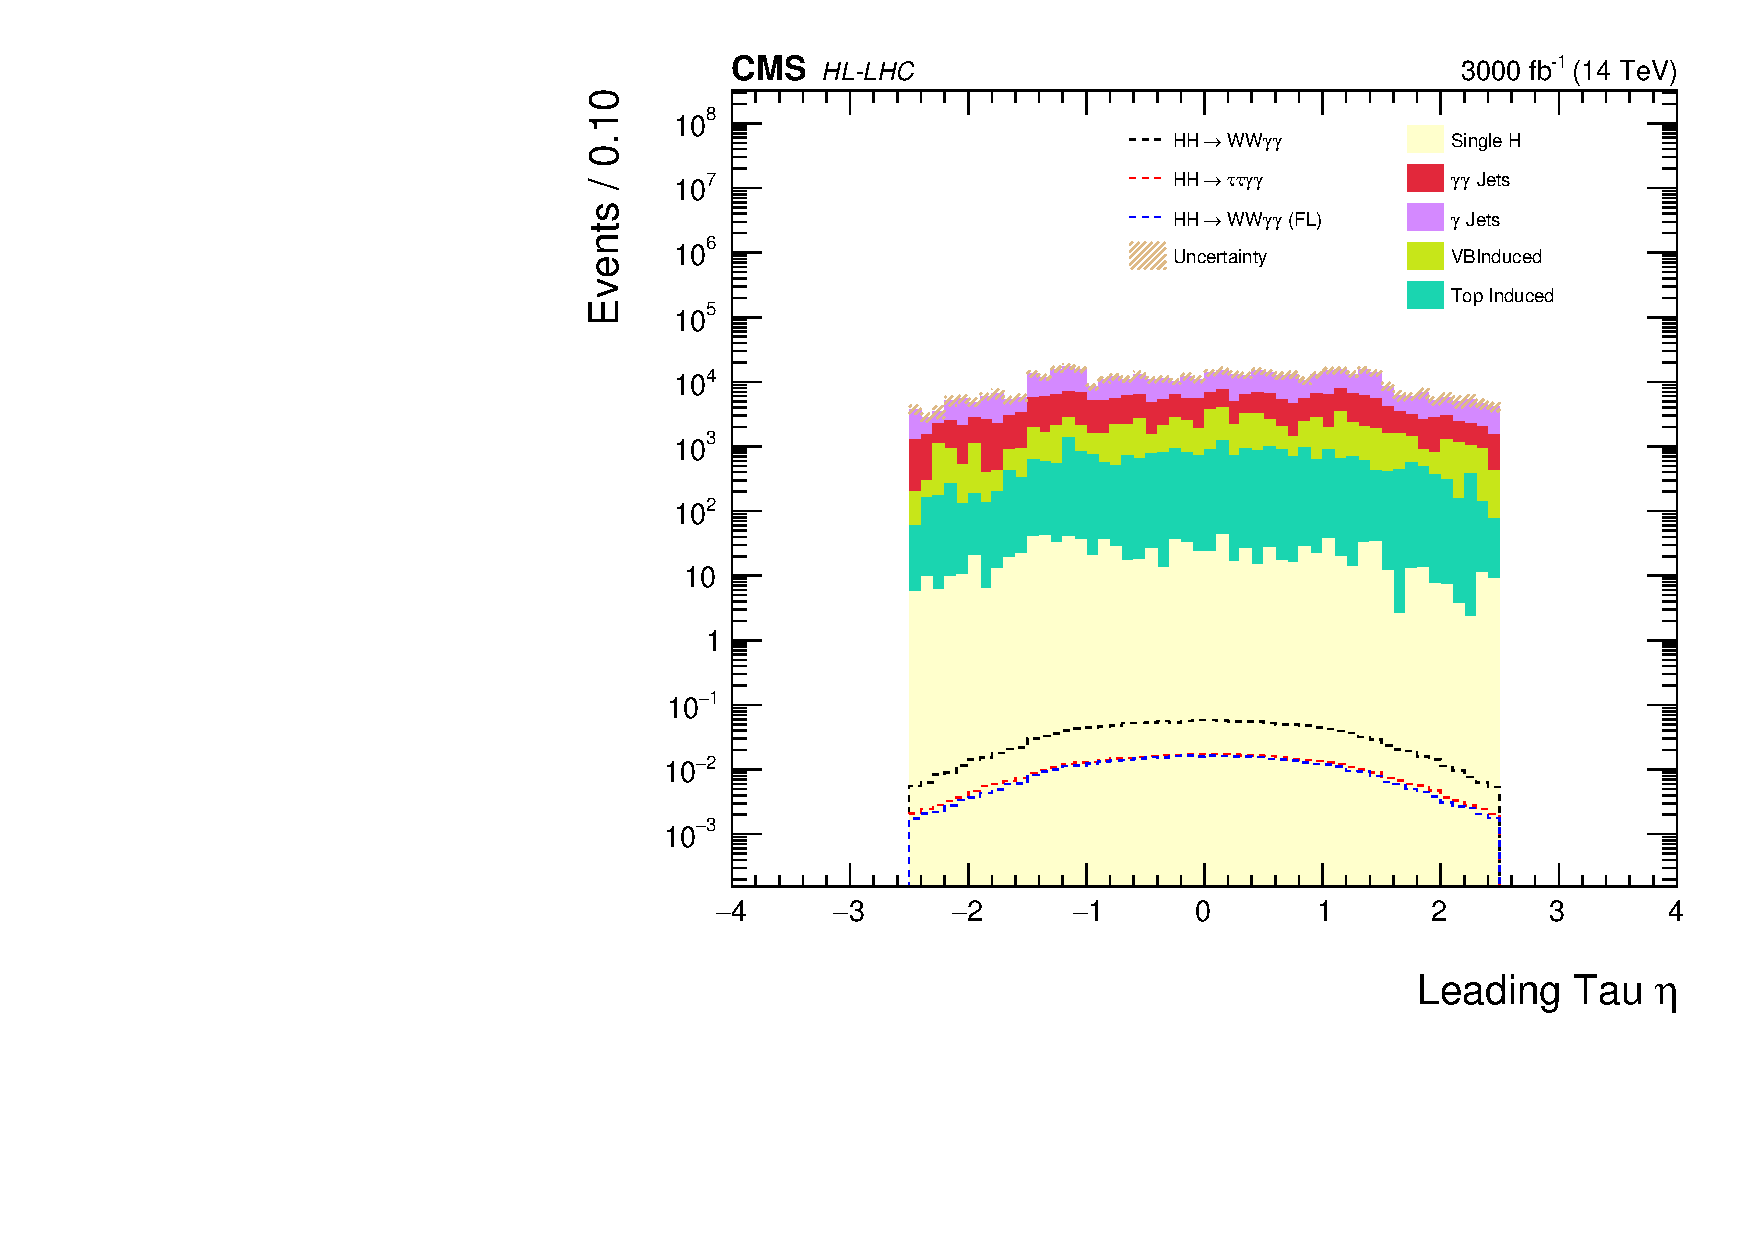
\includegraphics[width=\textwidth]{c3_leadingtau_eta_logy.pdf}
        \vspace{-0.5cm}
        \firstsubcaption{Leading Tau $\eta$}
    \end{subfigure}
    \vskip\baselineskip
    \begin{subfigure}[b]{0.475\textwidth}   
        \centering 
        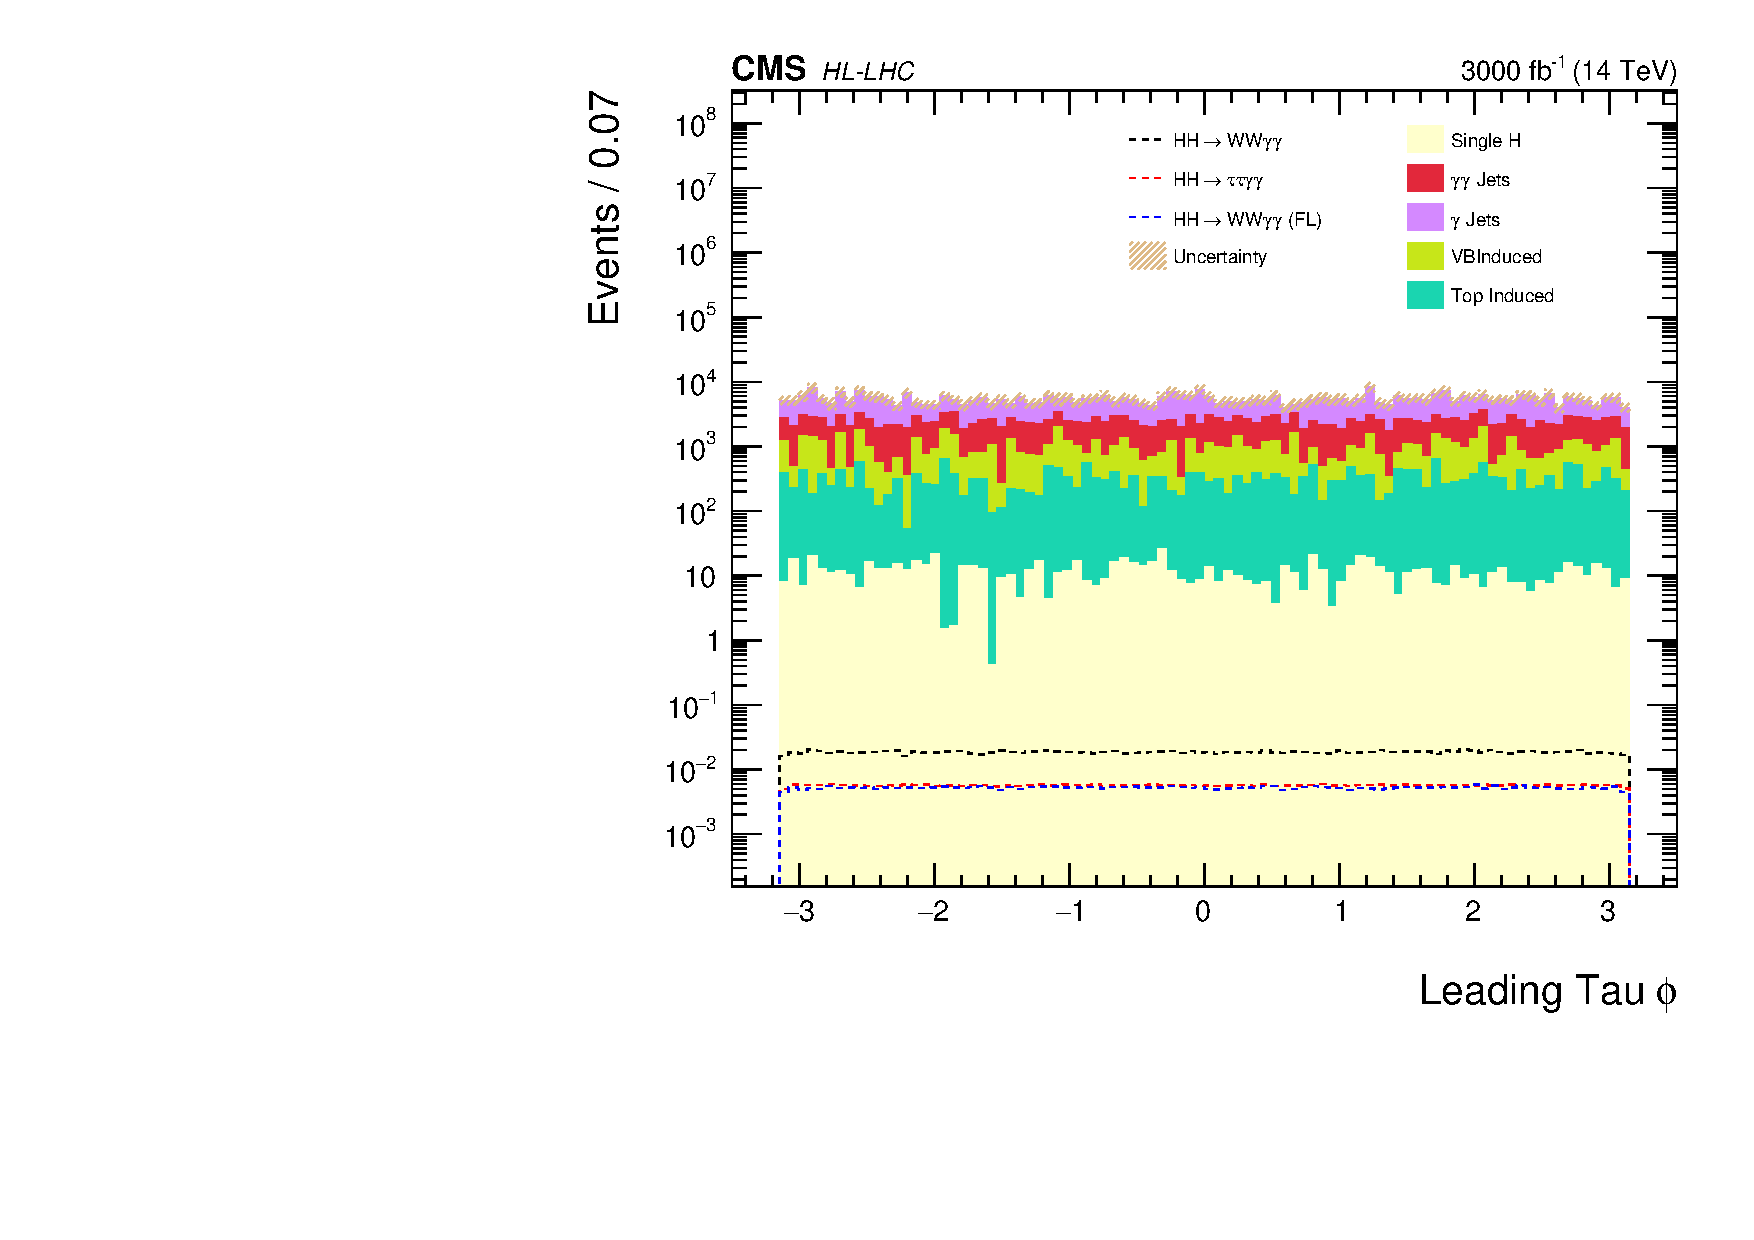
\includegraphics[width=\textwidth]{c3_leadingtau_phi_logy.pdf}
        \vspace{-0.5cm}
        \firstsubcaption{Leading Tau $\phi$}
    \end{subfigure}
    \hfill
    \begin{subfigure}[b]{0.475\textwidth}   
        \centering 
        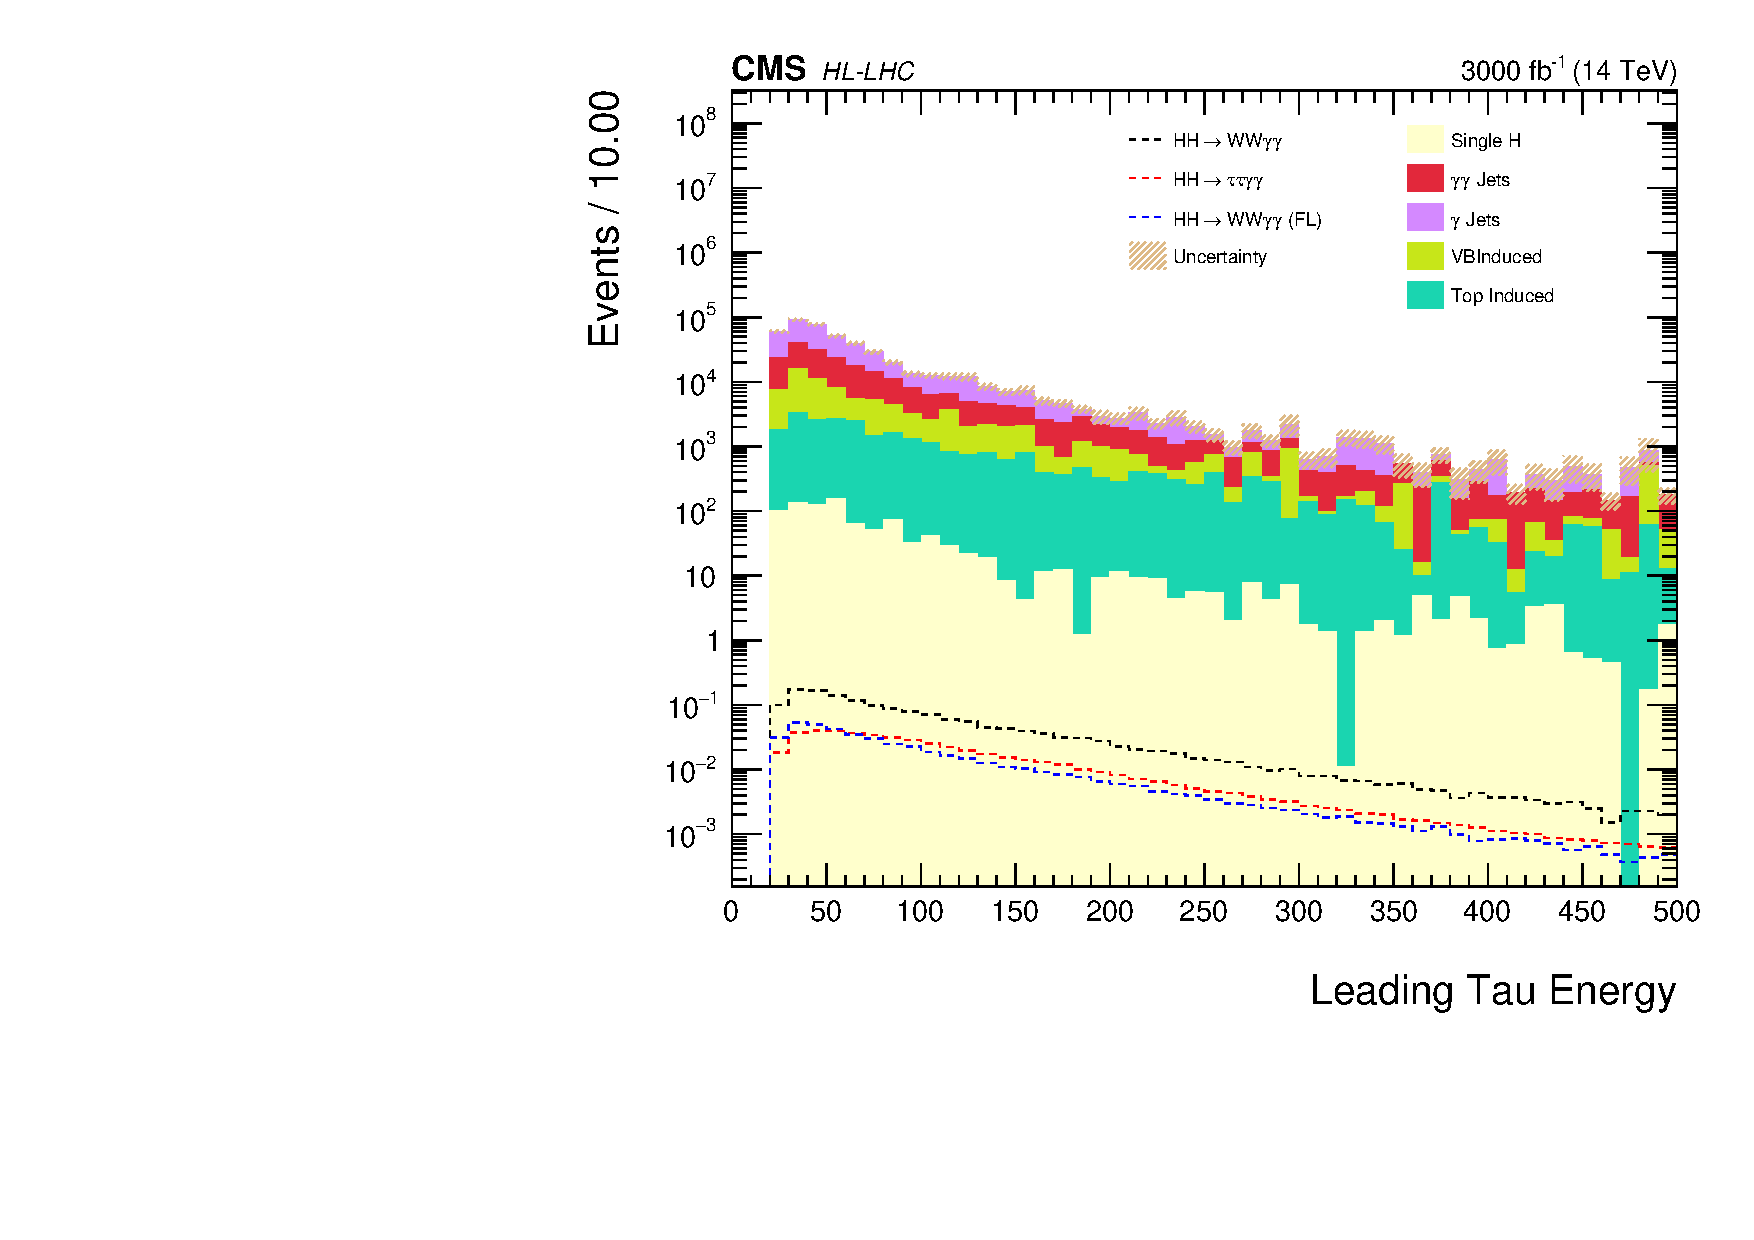
\includegraphics[width=\textwidth]{c3_leadingtau_E_logy.pdf}
        \vspace{-0.5cm}
        \firstsubcaption{Leading Tau energy}   
    \end{subfigure}
    \caption{\small DNN input distributions for the 1$\tau$ channel of $HH\rightarrow{\tau\tau\gamma\gamma}$ (continued).}
\end{figure*}


\begin{figure*}[h!]
    \centering
    \begin{subfigure}[b]{0.475\textwidth}
        \centering
        \includegraphics[width=\textwidth]{_logy.pdf}
        \vspace{-0.5cm}
        \firstsubcaption{Jet multiplicity}
    \end{subfigure}
    \hfill
    \begin{subfigure}[b]{0.475\textwidth}  
        \centering 
        \includegraphics[width=\textwidth]{_logy.pdf}
        \vspace{-0.5cm}
        \firstsubcaption{B-tagged jet multiplicity}
    \end{subfigure}
    \vskip\baselineskip
    \begin{subfigure}[b]{0.475\textwidth}   
        \centering 
        \includegraphics[width=\textwidth]{_logy.pdf}
        \vspace{-0.5cm}
        \firstsubcaption{Leading jet \pt}
    \end{subfigure}
    \hfill
    \begin{subfigure}[b]{0.475\textwidth}   
        \centering 
        \includegraphics[width=\textwidth]{_logy.pdf}
        \vspace{-0.5cm}
        \firstsubcaption{Leading jet $\eta$}
    \end{subfigure}
    \vskip\baselineskip
    \begin{subfigure}[b]{0.475\textwidth}   
        \centering 
        \includegraphics[width=\textwidth]{_logy.pdf}
        \vspace{-0.5cm}
        \firstsubcaption{Sub-leading jet \pt}
    \end{subfigure}
    \hfill
    \begin{subfigure}[b]{0.475\textwidth}   
        \centering 
        \includegraphics[width=\textwidth]{_logy.pdf}
        \vspace{-0.5cm}
        \firstsubcaption{Sub-leading jet $\eta$}   
    \end{subfigure}
    \caption{\small DNN input distributions for the 1$\tau$ channel of $HH\rightarrow{\tau\tau\gamma\gamma}$ (continued).}
\end{figure*}

\begin{figure*}[h!]
    \centering
    \begin{subfigure}[b]{0.475\textwidth}
        \centering
        \includegraphics[width=\textwidth]{c3_met_logy.pdf}
        \vspace{-0.5cm}
        \firstsubcaption{$E_T^{miss}$}
    \end{subfigure}
    \vskip\baselineskip
    \begin{subfigure}[b]{0.475\textwidth}  
        \centering 
        \includegraphics[width=\textwidth]{roc-tau-odd.png}
        \vspace{-0.5cm}
        \firstsubcaption{Odd ROC curve}
    \end{subfigure}
    \hfill
    \begin{subfigure}[b]{0.475\textwidth}   
        \centering 
        \includegraphics[width=\textwidth]{roc-tau-even.png}
        \vspace{-0.5cm}
        \firstsubcaption{Even ROC curve}
    \end{subfigure}
    \vskip\baselineskip
    \begin{subfigure}[b]{0.475\textwidth}   
        \centering 
        \includegraphics[width=\textwidth]{onetau-odd-weights.png}
        \vspace{-0.5cm}
        \firstsubcaption{Odd training weight}
    \end{subfigure}
    \hfill
    \begin{subfigure}[b]{0.475\textwidth}   
        \centering 
        \includegraphics[width=\textwidth]{onetau-even-weights.png}
        \vspace{-0.5cm}
        \firstsubcaption{Even training weight}
    \end{subfigure}
    \caption{\small DNN input distributions for the 1$\tau$ channel of $HH\rightarrow{\tau\tau\gamma\gamma}$ (continued) (a), corresponding ROC curves (b,c) and DNN evaluation on odd (d) and even (e) data.}
\end{figure*}
